% thesis.tex
%
% This file is root file for an example thesis written using the
% IIT Bombay LaTeX 2Style file.
% Created by Amey Karkare (21 June 2007)
%
% It is provided without warranty on an AS IS basis.

%=====================================================================
% Read: http://www.cse.iitb.ac.in/karkare/iitbthesis/
%    FAQ.txt     for frequently asked quetions
%    Changes.txt for changes
%    README      for more information
%=====================================================================

%=====================================================================
% DOCUMENT STYLE
%=====================================================================
% IITB PhD Thesis format default settings are:
%   12pt, one-sided printing on a4 size paper

% For two-sided printing, with Chapter starting on odd-numbered pages,
% use the following line instead:  
\documentclass[openright,twoside]{iitbthesis}
%=====================================================================
% OPTIONAL PACKAGES
%=====================================================================
% To include optional packages, use the \usepackage command.
% For e.g., The package epsfig is used to bring in the Encapsulated
%    PostScript figures into the document.
%    The package times is used to change the fonts to Times Roman;
%=====================================================================

%=====================================================================
% End of Preamble, start of document

	\usepackage{soul}
	\usepackage{mathtools}
	\usepackage{graphicx}
	\usepackage{amsfonts}
	\usepackage{array}
	\usepackage{commath}
	\usepackage{amssymb}
	\usepackage{subfigure}
	\usepackage{multirow,tabularx}
	%\usepackage{xcolor}
	\usepackage{bm}
	\usepackage{slashbox}	
	\usepackage{epsfig}
	
	\usepackage[titletoc]{appendix}% http://ctan.org/pkg/appendices
	
	\usepackage{times}
	\usepackage{algorithm}
	\usepackage{algorithmic}
	\usepackage{amsmath}
	\usepackage{cite}
	\usepackage{multirow}
	\usepackage{url}
	\usepackage{framed}
	\usepackage[table]{xcolor}
	\usepackage{mypublicationbox}
	\usepackage{rotating}
	\definecolor{eplbg}{RGB}{125, 102, 94}
	\usepackage{floatpag}	
	
	%\rotfloatpagestyle{empty}
	\floatpagestyle{plain}
	

%=====================================================================
%  Single counter for theorems and theorem-like environments:
%=====================================================================
	\newtheorem{theorem}{Theorem}[chapter]
	\newtheorem{proposition}{Proposition}		
	\newtheorem{corollary}{Corollary}		
	\newtheorem{lemma}[theorem]{Lemma}		

\begin{document}

%=====================================================================
	% Include the prelude for Title page, abstract, table of contents, etc
% You need to modify it to contain your details
	% prelude.tex
%   - titlepage
%   - dedication (optional)
%   - approval sheet
%   - course certificate
%   - table of contents, list of tables and list of figures
%   - nomenclature
%   - abstract
%============================================================================


\clearpage\pagenumbering{roman}  % This makes the page numbers Roman (i, ii, etc)



% TITLE PAGE
%   - define \title{} \author{} \date{}
\title{Meeting Data Accuracy and Quality of Service Requirements for Analytics in Transmission Grids}
%\title{Designing Data Dissemination Frameworks for Smart Transmission Grids}
%\title{Considering Data Quality and Quality of Service in Designing Data Dissemination Framework for Smart Transmission Systems}
\author{Rohit Gupta}
\date{2020}

%  - Roll number, required for title page, approval sheet, and
%    certificate of course work 
\rollnum{124050002} 

%   - The default degree is ``Doctor of Philosophy''
%     (unless the document style msthesis is specified
%      and then the default degree is ``Master of Science'')
%     Degree can be changed using the command \iitbdegree{}
\iitbdegree{Doctor of Philosophy}

%   - The default report type is preliminary report.
%      * for a PhD thesis, specify \thesis
\thesis
%      * for a M.Tech./M.Phil./M.Des./M.S. dissertation, specify \dissertation
%\dissertation
%      * for a DIIT/B.Tech./M.Sc.project report, specify \project
%\project
%      * for any other type, use  \reporttype{}
%\reporttype{Pre Synopsis Report}

%   - The default department is ``Unknown Department''
%     The department can be changed using the command \department{}
\department{DEPARTMENT OF ELECTRICAL \& ENGINEERING}

%    - Set the guide's name
\setguide{Prof. Krithi Ramamritham}
%    - Set the coguide's name (if you have one)
% \setcoguide{Prof. S. A. Soman}
%    - Set external guide (if you have one)
%\setexguide{Prof External Guide}

%   - once the above are defined, use \maketitle to generate the titlepage
\maketitle

%--------------------------------------------------------------------%
% DEDICATION
%   Dedications, if any, must be first page after title page.
\begin{dedication}
Dedicated to my ABC.
\end{dedication}

%--------------------------------------------------------------------%
% APPROVAL SHEET
%   - for final thesis, you need Approval Sheet. So, uncomment the
%     \makeapproval command.
%     it should come after dedication, if dedication is
%     present. Otherwise it is the first page after title page.
%\makeapproval


\chapter*{Declaration Certificate}

\noindent I declare that this written submission represents my ideas in my own words and where other's ideas or words have been included, I have adequately cited and referenced the original sources. I also declare that I have adhered to all principles of academic honesty and integrity and have not misrepresented or fabricated or falsified any idea/data/fact/source in my submission. I understand that any violation of the above will be cause for disciplinary action by the Institute and can also evoke penal action from the sources which have thus not been properly cited or from whom proper permission has not been taken when needed.\\

\vspace{10ex}
\hspace*{4 in}\ldots \ldots \ldots \ldots\ldots \ldots \ldots \ldots \vspace{0.1in}\\
\hspace*{4.4 in}(Signature of Student)\\\\\\
%\vspace{10ex}
\hspace*{4.6 in}\underline{\bf Rohit Gupta}\\
\vspace{4ex}
\hspace*{4.4 in}(Name of Student)\\\\\\
\vspace{4ex}
\hspace*{4.2 in} Roll No. \underline{\bf 124050002}\\
Date: March $2020$.
%%
%%
%--------------------------------------------------------------------%
% CERTIFICATE OF COURSE WORK
%   - for final thesis, a course certificate is required.
%   - specify the  PhD joining date for the certificate.
%     Contact you department office or academic office if you do not
%     know it.
\joiningdate{Jun 2012}
\begin{coursecertificate}
%  - command to add a course
%     it accepts 3 arguments:  Course ID, Course Name, Course Credits.

\addcourse{CS 601}{Algorithms and Complexity}{6}
\addcourse{CS 684}{Embedded Systems}{6}
\addcourse{CS 620}{New Trends in Information Technology}{6}
\addcourse{CS 681}{Performance Analysis of Computer Systems and Network}{6}
\addcourse{CS 720}{Spatial Databases}{6}
% \addcourse{HS 699}{Communication and Presentation Skills}{4}
\addcourse{CS 631}{Implementation Techniques for Relational Database Systems}{6}
\addcourse{CS 675}{Computer Graphics}{6}
\addcourse{CS 695}{Topics in Virtualization and Cloud Computing}{6}
\addcourse{CS 801}{Seminar}{4}

%\addppcourse: required for courses like HS 699 for which Acad office
%              requires PP, and not the actual credits.
%     3 arguments:  Course ID, Course Name, Course Grade(PP/NP).
\addppcourse{HS 699}{Communication and Presentation Skills}{PP}
\end{coursecertificate}

%--------------------------------------------------------------------%
% COPYRIGHT PAGE
%   - To include a copyright page use \copyrightpage
% \copyrightpage

%--------------------------------------------------------------------%
% ABSTRACT
\begin{abstract}
  A large number of electrical appliances are installed in buildings. With time, more appliances are added and old appliances and replaced. The dynamic nature of the electrical system in a building results in a variation in the age of the appliances. These appliances are bound to degrade with time and fail eventually. Once appliances are installed there is no way to automatically monitor the health of these appliances or to detect malfunctioning appliances and perform corrective action.

The current practice adopted by the maintenance staff is to maintain the blueprint of the electrical layout and refer to it when a problem is reported. Major components of the electrical system are hidden and can only make sense when correct blueprints are referred. The electrical layout in the building may change with time resulting in a change in the consumption pattern of each section of the building. It becomes difficult to keep on updating the electrical layout, therefore, it could be incorrect many times.

When a problem is reported, the maintenance staff measures the current flowing through different cables to identify the location and nature of the problem. It is not practical and economical to monitor various electrical parameters at all locations in the system to detect such problems. Therefore the maintenance is done mostly in a reactive manner. The failed appliances are replaced or repaired only when such incidents are reported. The current mechanism to identify these failure and performance loss depends on occupants reporting such incidents and is reactive and proactive.

As there is no easy way to monitor the health of the electrical system, the malfunctioning appliances which are not observed by the occupants, stay in the system and keep on wasting power. They wast energy and also put extra load on the system which also decreases the life of the system.

\end{abstract}


%--------------------------------------------------------------------%
% CONTENTS, TABLES, FIGURES
\tableofcontents
\listoftables
\listoffigures
\listofalgorithms

%--------------------------------------------------------------------%
% NOMENCLATURE
% \begin{nomenclature}
% \begin{description}
% \item{\makebox[0.75in][l]{IT}}{Instrument Transformer} 
% \item{\makebox[0.75in][l]{RMC}}{Remote Meter Calibration} 
% \item{\makebox[0.75in][l]{LPE}}{Line Parameter Estimation} 
% \item{\makebox[0.75in][l]{RCF}}{Ratio Correction Factor} 
% \item{\makebox[0.75in][l]{CT}}{Current Transformer} 
% \item{\makebox[0.75in][l]{VT}}{Voltage Transformer} 
% \item{\makebox[0.75in][l]{CVT}}{Capacitor Voltage Transformer} 
% \item{\makebox[0.75in][l]{BED}}{Bias Error Detection} 
% \item{\makebox[0.75in][l]{PMU}}{Phasor Measurement Unit} 
% \item{\makebox[0.75in][l]{PDC}}{Phasor Data Concentrator} 
% \item{\makebox[0.75in][l]{LPDC}}{Local Phasor Data Concentrator}
% \item{\makebox[0.75in][l]{SPDC}}{Super Phasor Data Concentrator}
% \item{\makebox[0.75in][l]{BAM}}{Bus Angle Monitoring}
% \item{\makebox[0.75in][l]{MCGG}}{Monitoring Coherent Groups of Generators}
% \item{\makebox[0.75in][l]{PSSE}}{Power System State Estimation}
% \item{\makebox[0.75in][l]{LSE}}{Linear State Estimation}
% \item{\makebox[0.75in][l]{CEUT}}{Centralized Execution with Unfiltered data forwarding Technique}
% \item{\makebox[0.75in][l]{DEFT}}{Distributed Execution with Filtered data forwarding Technique}
% \item{\makebox[0.75in][l]{ROCOF}}{Rate Of Change Of Frequency}
% \item{\makebox[0.75in][l]{COI}}{Centre of Inertia}
% \item{\makebox[0.75in][l]{LS}}{Least Squares}
% \item{\makebox[0.75in][l]{TLS}}{Total Least Squares}
% \item{\makebox[0.75in][l]{LAV}}{Least Absolute Value}
% \item{\makebox[0.75in][l]{NLS}}{Nonlinear Least Squares}
% \item{\makebox[0.75in][l]{NLAV}}{Nonlinear Least Absolute Value}
% \item{\makebox[0.75in][l]{ODR}}{Orthogonal Distance Regression}
% \item{\makebox[0.75in][l]{ILP}}{Integer Linear Programming}
% \item{\makebox[0.75in][l]{SCADA}}{Supervisory Control and Data Acquisition}
% \item{\makebox[0.75in][l]{WAMS}}{Wide Area Measurement System}
% \item{\makebox[0.75in][l]{ICN}}{Information Centric Networking}
% \item{\makebox[0.75in][l]{NASPI}}{North American SynchroPhasor Initiative}
% \item{\makebox[0.75in][l]{NASPInet}}{NASPI Network}
% \item{\makebox[0.75in][l]{PGW}}{Phasor Gateway}
% \item{\makebox[0.75in][l]{DB}}{Data Bus}	
% \end{description}
% \end{nomenclature}

\cleardoublepage\pagenumbering{arabic} % Make the page numbers Arabic (1, 2, etc)

%=====================================================================
% Include the technical part of the report
	
	\chapter{Introduction}
\section{System Problems}
% of electrical systems and faults 

Electricity is one of the most utilized form of energy. It is popular because of the ease of distribution and on-demand availability. The electrical distribution systems are efficient, convenient, safe, and environment-friendly compared to all other energy sources. Unfortunately, it is not easy to store and carry electricity around. , Therefore it should be produced and distributed at the time of its demand. The electricity production and distribution system should always be in the ready state to cater to the everchanging demand. 



Electricity distribution systems existed for a long time. These systems are time tested and are very stable in delivering the power to the individual appliance consistently. They are very reliable and modern life is highly dependent on these electrical distribution systems. Unfortunately, these electrical distribution systems are without any backup and are always in use. So they rarely get downtime for preventive maintenance or health monitoring. Therefore they are mostly maintained in case of breakdown.

There are mechanisms built into electrical distribution systems to handle Critical errors that should be handled in real-time to prevent the entire system from breakdown and accidents. Circuit breakers are the equipment that identifies such a critical fault and disconnects the faulty part form the rest of the system. These circuit breakers are installed at the strategic location to isolate the faulty section and restrict the impact of the faults on the rest of the system. Some circuit breakers are also designed to minimize the impact of accidents on the occupants caused by faults or improper handling of the system. Such circuit breakers are commonly installed in residential and commercial spaces.

The circuit breakers are disruptive in nature and stops all the operations in the faulty section. Therefore they are designed to prevent only the most severe and catastrophic faults in the electrical systems. Less severe problems and losses in the electrical distribution systems are tolerated in order to maintain the continuous operation of these systems. These losses are considered insignificant relative to the efforts required to mitigate such losses. These losses are very small and insignificant at the household and building level but are huge at the global level.


\subsection{Types of Problems}
AS these systems are continuously in the running state, Problems are encountered because of the misuse of the system or wearing of the system because of overload or other environmental conditions. Out of a large number of problems observed in the electrical distribution systems, most common problems could be categorized as follows

\begin{itemize}
\item Short circuit: This type of fault occurs when the supply wire is connected to the neutral wire which results in the flow of a very large current through the distribution wires. There are always some losses in the wiring, Therefore the energy flowing into the system is released by the wires as losses resulting in heating up and eventually catching fire. The wires in any distribution system are not capable of sustaining such a large current for a long duration. To prevent such a huge flow of current, the section of the distribution circuit is disconnected from the rest of the circuit either by the fuses or the circuit breakers.

\item Earthing Fault: When the phase line is somehow connected to the earth or ground, the earth acts as a big sink and the current starts to flow from the phase to the earth. This flow of current also causes the heating up of the wire. Many times it could be because of humans or animals getting in contact with the live wire. Such flow of current could be lethal and should be interrupted immediately. Special relays are installed to detect the occurrence of this event. These relays act immediately and disconnect the impacted circuit from the rest of the system.

\item Circuit Overload: Local electrical distribution systems are like trees where the distribution transformer is the root of the tree and all the appliances are at the leaf nodes. Each branch of the electrical system tree is installed with the maximum current required by the appliances installed under the branch. If the current drawn through the wiring is higher than the maximum capacity it should be because of some unexpected load connected to the system. The losses in the wire are proportional to the square of the current flowing through it. The higher current result in higher distribution losses and heating up of the wire. This heating will damage the insulation and may result in other faults or might cause a fire. To prevent this type of overcurrent, circuit breakers are installed which disconnects the circuit when current beyond a stipulated limit is observed. 

\item Appliance Overload: The appliances installed may start consuming more power because of the increase in the losses because of the aging of the appliances. This will not result in the circuit overload but causes loss of energy and therefore increase the energy bills.

\item Installation Errors: Many times it is observed that the circuit breaker installed is of the wrong capacity. The circuit may be drawing current up to its maximum capacity and installing any new appliance will result in regular overcurrent and tripping of the circuit breaker. Unfortunately, there is no way to identify such boundary conditions in the circuits other than measuring the current at each level in the distribution tree.

\item Failed Appliance: Appliances may fail to perform their desired tasks such as failed lighting equipment or air conditioners which are not cooling. The appliances which can be observed by the occupants are reported to the maintenance staff and are either repaired or replaced. But in many cases, the appliance may go on unobserved and therefore continue to stay in the system. In cases where some service should be performed by multiple parallel appliances like multiple air conditioners are installed to cool a zone, failure of one of the airconditioner will put extra load on other air conditioners but might not impact the occupant's comfort.

\item Underperforming appliances: Many appliances that use mechanical components may decrease in efficiency with time. The appliances that have to perform a predefined task will have to pull more current to compensate for the increase in the losses. This increase in the current is difficult to measure manually and remains undetected. Many such appliances will deteriorate the power factor with time resulting in the same power consumption but more power flowing through the wire. In both of these cases, more power flowing through the wires is not possible to detect manually and the problematic appliance stays in the system.

\item Phase imbalance: Although the electrical distribution system has 3-phases, many appliances are of single-phase type. These single-phase appliances create phase imbalance which is not good for the health of the system. In order to reduce the imbalance caused by the single-phase appliances, the system architect puts an equal load on each phase to maintain balance among phases. New appliances are often added to the system which may increase this phase imbalance. There is no way for the maintenance staff or electricians to check the phase imbalance at each level of the distribution system, therefore, the phase imbalance continues to adversely impact the system.

\item Starting Failures: Many appliances come with their own safety mechanism. For example, when a compressor in an air conditioner, fails to generate enough pressure while starting with its maximum current, the safety circuit shuts down the compressor. Unfortunately, this does not prevent the air conditioner to attempt the start again after a few minutes. Such failed appliances will create a repeated current surge that can damage the system.
\end{itemize}

The problems that are result in the disconnection from the main supply are quickly taken care of and the remaining problems are left unhandled because of the current approach for solving these problems.
\section{Current Approach}
The maintenance of the electrical system is generally done only when the system break downs. This is because of multiple reasons. The electricity should be made available without interruptions. Maintenance of the distribution may require either operation in the live system or shutdown of the system. Until the exact health of the system is known, it is difficult to identify the rectifications required in the system. Because of this preventive maintenance are less common for the electrical distribution systems. 

The problems mentioned in the above section can be detected if the power consumption of each appliance is monitor. IT is straightforward to identify the problematic section or appliance based on the trend of power consumption. But it is very costly to continuously measure the power consumed by each appliance. It is also not practical to measure the power consumption of each appliance at a regular interval. With the introduction of thermostat based appliance and intelligent appliances, it is also not possible to identify the overall power consumption behavior of the appliance by measuring the power consumption in one measurement. 

With the invention of smart meters that can sense and report power consumption at a higher sampling rate, it became possible to observe the power consumption and derive various inferences from the power consumption pattern. It is now possible to identify how much power is demanded by a particular appliance and when.

Each appliance can produce different power consumption patterns which can be observed to identify ON and OFF appliance by just observing the power in the mains meter data. Thus it is also possible to identify the variation of power consumption pattern of an individual appliance. This introduced a new field of research to compute the power consumption of individual appliances from the mains meter data.

This Idea of identification of appliance state and thereby computing the power consumption was first utilized by the Hart. The active and reactive power consumption pattern was used to both identify the status of the appliance and compute power consumed by the appliance. This field of None Intrusive appliance load monitoring (NIALM) and a number of sensing techniques and algorithms are tried to achieve this goal. The focus of this field of research is to measure the power consumption of individual appliances by minimal sensing. Unfortunately, NILAM depends on expected behavior of the appliances and fails to work when the appliance misbehaves or some other unexpected elements are introduced into the system.
\section{Proposed Solutions}
\begin{figure} 
	\centering
	\includegraphics[width=1\linewidth]{tikz/outline}
	\caption[Outline]{Outline}
	\label{fig:outline}
\end{figure}

The problem of identification location of the faults or anomalies in the system is a complex problem that requires taking care of challenges on different fronts. It includes improving data acquisition mechanisms in terms of more accurate and frequent and timely data collection, data management and analysis of the data. Therefore, the problem is divided into the following subproblems.

\textbf{To design a sensor that can sense the electrical parameter at the desired accuracy and frequency}

With the introduction of the smart grid, smart meters are being installed at a large scale to collect power consumption data. Most of the commercial smart meters are designed to collect data at a reasonably high frequency of a sample every few minutes ranging from 1 to 15 minutes. On the other hand, there are industrial meters that can provide data every second but are not cost-effective. Most of the NILAM research is done on 1 Hz or higher frequency data collected with high-grade lab equipment. It is not practical to deploy any of this equipment for fault identification.
 
In order to facilitate the NILAM and fault identification, we have designed a smart meter that can provide data up to 10kHz frequency. At such a high frequency the volume of data collected will be too high. To reduce the data volume, a capability is added in the smart meter to transmit the data only when a significant change in power consumption is detected. 

Industrial smart meters provide data only through MODBUS protocol over RS485 ports, This results in a lot of bandwidth limitations and therefore could not be used for high-frequency data. The meter is designed to support multiple modes of communication including wireless communication and deliver large volume of data without congesting the channel bandwidth.  




\textbf{To identify a sensing method that is generic and does not require the learning of signatures}


A lot of attempts are made to sense the status of the appliance in the electrical systems. With the availability of the smart meters, a more fine-grain power consumption data is available from these electrical systems. It is possible to identify when appliances are switched ON or OFF by analyzing the time series power consumption data collected from these smart meters. With the introduction of IoT devices, it is now possible to install a large number of sensors and colled data from them. This enabled the utilization of a verity of sensors in collecting the data from these sensors. 

Unfortunately, all effort is towards the measurement of the energy consumed by the appliance. These approaches use some behavior of the appliance to identify if the appliance is on or off and compute the energy consumed by the state of the appliance. Most of the techniques are highly dependent on the signatures learned to identify the appliance state. Many of the technique requires learning of the signature of each appliance or on-site learning which makes them less suitable for large scale deployment.

These techniques fail to identify the state of the appliance in many situations like change in the signature, change in location, presence of multiple appliances, etc. Therefore, the information made available by these techniques does not provide any insight into the health or the performance of the system. A technique that does not require learning the signature of each appliance is more suitable for large scale deployments.

A well-known observation of variation in voltage observed at the load level can be utilized to identify the load. Unfortunately, there is a large variation in the supply voltage and a large number of variations are observed in the voltage because of the load variation in the rest of the system. This presents a big challenge of removing noise to correctly identify the load state of the subtree. The method of identification of removal of noise is devised to utilize the voltage sensed at various locations. 

In this work, we have introduces the technique to use voltage values sensed at different locations in the system and spatial variation in the voltage to determine the state of the system, incorrect system configurations. The system state information together with the power consumption measured in the mains meter is utilized to determine the load consumption of each section of the system. The temporal variation in the voltage is utilized to determine the correct layout of the system. This information is required to rectify the phase imbalance situation. Temporal variation in voltage is also used to detect current spikes to determine the location of the failed appliance. As voltage can be sensed by plugging a device into the socket, the task of layout identification and spike detection can be performed easily with minimal equipment and effort.

We present a voltage sensing technique that can be installed without learning the signature of the appliance. Voltage variation is a generic effect caused by each appliance, therefore, it can be employed for identification of the state of any appliance. It can also be used to identify the zone level power consumption which is useful for the identification of the location of the problem in the system.


\textbf{To design a sensor data collection system that can reliably collect data from multiple sensors}

Collecting data from a large number of sensors without interruption and errors is a difficult task. There are many weak points where the data collection system may breakdown. Communication may get interruption, the device may not get continuous power supply or the IoT device may fail with time. For such problems, the system should be capable of recovering itself and 

The person installing the equipment install the equipment to correctly three-phase or may tag the sensor wrongly. With three-phase systems, the probability of putting the wrong phase number on the meter is very high because the person installing the meter may not receive correct information or may not receive the information at all. In such a scenario an IoT installation mechanism is required which can enable any person who is not an expert in the system and can install them without need to perform any technical task. The gateway IoT device should automatically detect the topology of the network connecting these devices and should also adapt to the changes to such topology without any intervention.



\textbf{To design algorithms to identify problems in the system}

There are multiple problems that can be present in the distribution systems in the buildings. These problems could be of continuous overload because of unwanted or underperforming appliances. They could be sudden short-term spikes of current because of faulty appliances or unbalanced load in the system because of the inappropriate setup of the appliance and instrumentation.  

These problems mostly go undetected by the maintenance staff, therefore, no corrective actions are taken to eliminate them. As the total power consumption is already measured by a smart meter at a higher sampling rate, it is possible to identify some unexpected behavior in the system using only the smart meter data. 

In this work, we present the algorithm to identify the spikes in the mains meter data and thus identify the presence of faulty appliance in the system. With the technique to compute zone level energy and using the voltage sensing technique, it is possible to find the source of the spike and unexpected changes in the load profile of the zone to detect if the source of the problem is present in the zone. 

Using the voltage sensed at multiple places we have also developed the mechanism to identify the phase of individual sockets thus enabling the correction of the phase of the wrongly labled smart meters or lines and improving the overall phase imbalance of the system.
\textbf{To identify the location where sensors should be install}

Electrical distribution systems supply power to a large number of appliances installed in any building. The number of appliances can very easily go beyond tens in any household and hundreds in any commercial building. Various sensing options are suggested identifying the state of the appliance and the power consumption of appliances. But these approaches face limitations because of the training required to learn the signature of these appliances. There are only a limited number of sensors like smart meters that do not require learning a signature. 

Many of these appliances are identical and difficult to differentiate based on their power consumption pattern. In such a case it becomes difficult to identify a single sensing parameter that can distinguish between these appliances. 

We present the optimization formulation for the sensor placement problem and prove that it is an np-hard problem. We also present a greedy algorithm that provides a reasonable number of the sensor required for any setup. 
   



	\chapter{Related Work}
\section{Power Distribution}
\begin{figure}
	\centering
	\includegraphics[width=0.7\linewidth]{tikz/phase_r}
	\caption[Voltage and current for a resistive load]{Voltage and current for a resistive load}
	\label{fig:phaser}
\end{figure}

\begin{figure}
	\centering
	\includegraphics[width=0.7\linewidth]{tikz/phase_l}
	\caption[Voltage and current for a inductive load]{Voltage and current for a inductive load}
	\label{fig:phasel}
\end{figure}

\begin{figure}
	\centering
	\includegraphics[width=0.7\linewidth]{tikz/phase_c}
	\caption[Voltage and current for a resistive load]{Voltage and current for a resistive load}
	\label{fig:hart1}
\end{figure}

\begin{figure}
	\centering
	\includegraphics[width=0.7\linewidth]{tikz/phase_harmonic}
	\caption[Voltage and current for a load with higher harmonic]{Voltage and current for a load with higher harmonic}
	\label{fig:phase_harmonic}
\end{figure}

\begin{figure}
	\centering
	\includegraphics[width=0.7\linewidth]{tikz/phase_dc}
	\caption[Voltage and current for a load with higher harmonic]{Voltage and current for a load with higher harmonic}
	\label{fig:phase_dc}
\end{figure}

\begin{figure}
	\centering
	\includegraphics[width=0.7\linewidth]{tikz/pq}
	\caption[Active, reactive and appearent power]{Active, reactive and appearent power}
	\label{fig:pq}
\end{figure}

Electrical power is generated in bulk at large power plants and transmitted to load centers through the high voltage transmission cables. 
The power is supplied through the alternating current induced by the voltage that varies as a sine wave. The current drawn by the load is also alternating but the pattern of the waveform is dependent on the electrical nature of the load. If the load is resistive, the current is also a sine wave and the sine wave coincides with the voltage wave as shown in the figure (res curr). The behavior of a capacitive load is also a sine wave but it leads by an angle of 

%$\pi/2$

if the voltage is given by 

$$v(t) = v_{m}\sin\left(t\right)$$

There $v(t)$ is the instantaneous voltage $t$ is the time and $v_{m}$ is the magnitude of the voltage.
The current drawn by the capacitive load is given by 

$$i_c(t) = c_{m}\sin\left(t+\ \frac{\pi}{2}\right)$$

where $c_{m}$ is the magnitude of the current waveform.

Similarly, the current drawn by an inductive load is also sine wave but it legs the voltage by $\pi/2$ angle. which is given by 

$$i_l(t) = l_{m}\sin\left(t-\ \frac{\pi}{2}\right)$$
 
The power delivered to the appliance is the instantaneous product of the voltage and the current. The voltage and current waves are aligned for the resistive load therefore the power delivered is maximum. Figure (p curve r) shows that the power drawn is always positive. But In the case of capacitive or inductive load, the current and voltage are out of phase by a right angle, therefore the power delivered is zero. 
Figure (p curve c) shows that the power drawn is both positive and negative therefore the net flow of power for the complete voltage cycle is zero.


When the current wave is in the same phase as the voltage, total power drawn is delivered to the load this power is termed as active power and load that draws this type of power is termed as the active load. Similarly, the power drawn by the inductor or the capacitor which is pushed back to the system by the load is termed as the reactive power and the load drawing such load is term as reactive load. The active and reactive power of the load are represented as the vectors, where the x-axis represents the reactive power and the y-axis represents the active power. The vector sum of these two powers is the total power flowing to the load. this power is called the apparent power as shown in the figure (PQ). Apparent power $P_{apparent}$ can also be computed as follows 

$$P_{apparent} = V_{RMS} * I_{RMS} $$

Where $V_{RMS}$ is root mean square (RMS) value of the voltage and $I_{RMS}$ is the RMS value of the current drawn by the load.

Most of the conventional appliance has both resistive and inductive components therefore they draw both the active and reactive power during their operation. 
\section{NIALM}
\begin{figure}
	\centering
	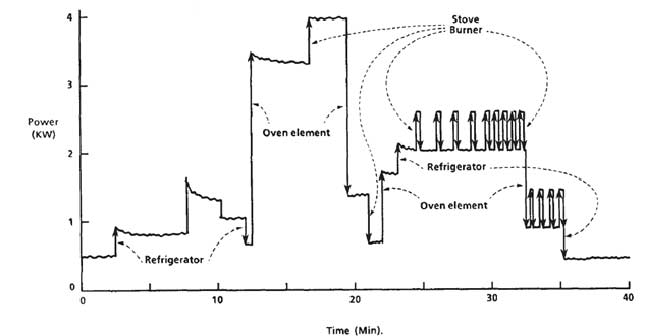
\includegraphics[width=0.7\linewidth]{images/hart1}
	\caption[Time serise power consumption of differnt appliance]{Time serise power consumption of differnt appliance}
	\label{fig:hart1}
\end{figure}

\begin{figure}
	\centering
	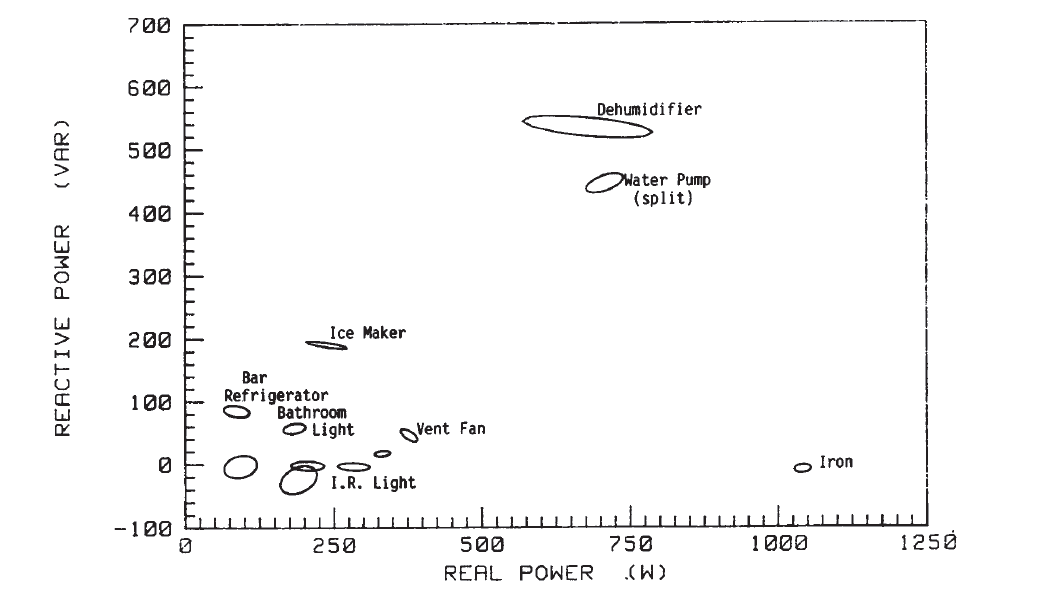
\includegraphics[width=0.7\linewidth]{images/hart2}
	\caption[Active and reactive power consumption of different appliances]{Active and reactive power consumption of different appliances}
	\label{fig:hart2}
\end{figure}

\begin{figure}
	\centering
	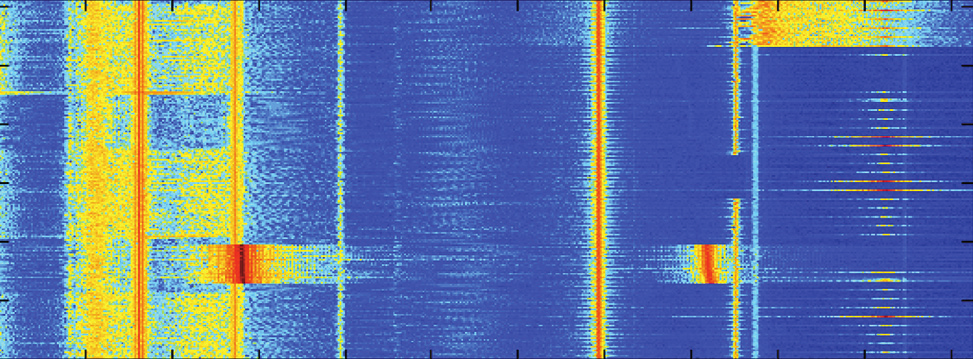
\includegraphics[width=0.7\linewidth]{images/noise}
	\caption[EM Noise]{EM Noise}
	\label{fig:noise}
\end{figure}

With the advancement of instrumentation technology, it became possible to collect power consumption data at an interval of one second. The time-series power data collected at this frequency clearly displays different patterns depicting the operation of individual appliances, 
This motivated Hart \cite{hart} to compute the power consumption of individual appliances by measuring the power at only the mains and utilizing the patterns learned for the appliances. 
Figure \ref{fig:hart1} shows the power consumption pattern for some of the appliances
The term NIALM (Non-Intrusive Appliance Load Monitor) was introduced by Hart to represent the idea of measuring the power consumption of all the appliances without installing any measurement equipment in a house. 

Initially, the active and reactive power consumption measures at the 1 Hz frequency was used to learn and identify the appliance power consumption. The power signatures as shown int the figure \ref{fig:hart2} worked reasonably well for a limited number of distinct appliances with distinct power consumption signatures. This approach of using the 1 Hz power measurement fails to provide an accurate result when a large number of the appliances are present or multiple appliances of similar appliance signature are present. This resulted in a plethora of research which tried to use different signatures to identify the status of the appliances. The research changed from non-intrusive to least intrusive and a large number of sensing techniques and algorithms were introduced to achieve the goal of power measurement. 




The conventional appliances like heater, incandescent bulb, electric motors have only resistive and inductive components. The current drawn by these appliances is the sine wave. Many electrical motors draw the current of the higher-order frequency. This enabled the identification of such appliances by measuring the total harmonic distortion (THD) which is the ratio of the magnitude of the fundamental frequency to the divided by the amplitude of the current. Figure \ref{fig:phase_harmonic}. It is not possible to distinguish among the appliance that has different harmonics using only the active and reactive power. A smart meter that provides THD of the load are higher-end costly industrial smart meters could not be installed in the common household because of their cost constraints. 

While THD is an important parameter, it does not provide information about the higher-order frequencies present in the current. New appliances that consisted of electronic components draw complicated current wave as shown in the figure \ref{fig:phase_dc} which makes the use of THD less efficient therefore researchers shifted their focus toward collecting high-frequency data to construct signatures. 


A huge variation of current waveforms are observed from appliance to appliance but it is difficult to collect and utilize these signatures because of the following reasons  


\begin{itemize}
    \item High volume of data: To sense and analyze the entire current waveform a higher data sampling rate is required which is in the range of 10-50 kHz collecting and sending the data to the server at this rate is processing it is difficult on the currently available ES485 type of communication channel.

\item Decomposing the appliance level signature: The meter installed at the mains will sense the waveform generated by combining all the waveforms from the ON appliance at any given time. The task of breaking down this into each component is challenging and computationally very demanding.

\end{itemize}


Because of this, multiple approaches to compress the information are devised.
\section{Sensing Other Parameters}
Assuming that the power consumed by the appliance is constant and once it is known, only identifying the state of the appliance is sufficient to compute the total power consumed by the appliance during a period.

All electric appliances are to perform some task which in turn causes some physical change on the surroundings. These are all observable changes like light, heat, motion etc. Which is the expected work of the appliance? There could also be some unintended side effects which also affect the surrounding like noise caused by the fan, vibration caused by the compressor of the refrigerator.

\begin{itemize}
    \item Lighting appliance produces enough light to identify it states. Cheap light intensity sensors are available which can be used to identify the lighting appliance state but the accurate placement of such a sensor is very critical because these sensors can easily be misled by daylight or light from nearby lighting equipment.
    \item A sensor like an infrared emitter pair could be used to detect if a fan is moving out stationary or even to measure the speed of the fan. These sensors are impacted by other infrared light sources like the daylight but can be compensated for such different environment. A skilled worker is required to install such a sensor as these sensors should be placed accurately and may be required to calibrated during installation.
    \item Fan and many other appliances like mixer, grinder, or washing machine generate significantly audible noise.  This audio noise can be sanded to detect the appliance state. This is a less reliable sensor because it will sense the noise coming from all directions, and all loud sounds will be detected as noise. In countries like India where high audio noise from vehicles and celebrations is very common, this sensor will generate a large number of false-positive events.
    \item The effect of the room heater and the air conditioners can be observed by installing temperature sensors. Outside temperature can be used identified if the room is being cooled. When the air conditioner is cooling the temperature in the vicinity of the air blower will decrease gradually. It requires some interpretation but a temperature sensor can very accurately identify the state of the air conditioner. But it is not easy to identify the stare of all heating appliances. It is difficult to measure the temperature change for appliances like the water heater or cooking appliance or some cooling appliance like chiller or freezer because they provide thermal isolatin. Temperature measurement will fail to provide an accurate state for such an appliance.
    \item In many cases, the man component of the appliance is a motor which converts the electrical energy to some mechanical form. The compressor of the refrigerator or rotor of a washing machine. These motors generate vibration that can be sensed by sensors to detect the appliance operation.
    \item A number of appliances like a fan and air conditioners circulate the air by means of air flow. For such appliances, the wind speed can be measured to detect if the appliance is on or off. Installing flow sensor is difficult and requires expertise. These sensors are large in size and contain moving parts that make their installation difficult. Because of these reasons flow sensors are used only where no other sensor can be installed. If there is any possibility of measuring other parameters to derive the same information using alternate sensors like temperature, vibration, sound or any other sensor the alternate sensors are generally used.
\end{itemize}


% The naive approach to finding the consumption of each appliance is to measure the power at each appliance. There are multiple challenges involved in measuring each appliance.

\begin{itemize}
\item \textbf{Technical skills required to install a meter:} It is not easy to install a smart meter, it requires a set of precise connection, may involve working with live high voltage wires or a local blackout, and need a decent amount of time to install test and make the meter data available to the system. It is not a plug and play devices.
 \item \textbf{Not all the appliance can be metered:} Many appliances are plug level devices such as laptops. To measure the power consumption of such devices a meter should be attached to the device rather than on the wall mount which will be a cumbersome option.
 \item \textbf{Losing aesthetic sense of the building:} meters are bulky, they need big space to be installed and mounted on for safety reasons. installing a meter on each wall in each room will be visually unattractive and space will lose its aesthetic sense.
 \item \textbf{Huge volume of data to be collected:}, As the current day smart meter provides only the instantaneous power reading, each meter installed will generate massive data that should be communicated and processed at the server. This will require reasonably large communication bandwidth, storage capacity, and processing power to analyze the data.
 \item \textbf{Too much cost involved:} Each meter installation will require at least 10000 Rs of expenditure, the benefits of reducing the energy consumption and reducing the carbon footprint are not enough to motivate customers or the utility to invest such a hefty sum.
\end{itemize}



% Assuming that the power consumed by the appliance is constant and once it is known, only identifying the state of the appliance is sufficient to compute the total power consumed by the appliance during a period.

All electric appliances are to perform some tasks which in turn causes some physical change in the surroundings. These are all observable changes like light, heat, motion, etc. Which is the expected work of the appliance? There could also be some unintended side effects which also affect the surrounding like noise caused by the fan, vibration caused by the compressor of the refrigerator.

Lighting appliance produces enough light to identify it states. Cheap light intensity sensors are available which can be used to identify the lighting appliance state but the accurate placement of such a sensor is very critical because these sensors can easily be misled by daylight or light from nearby lighting equipment.

A sensor like an infrared emitter pair could be used to detect if a fan is moving out stationary or even to measure the speed of the fan. These sensors are impacted by other infrared light sources like the daylight but can be compensated for such different environment. A skilled worker is required to install such a sensor as these sensors should be placed accurately and may be required to calibrated during installation.


% The effect of the room heater and the air conditioners can be observed by installing temperature sensors. Outside temperature can be used identified if the room is being cooled. When the air conditioner is cooling the temperature in the vicinity of the air blower will decrease gradually. It requires some interpretation but a temperature sensor can very accurately identify the state of the air conditioner. But it is not easy to identify the stare of all heating appliances. It is difficult to measure the temperature change for appliances like the water heater or cooking appliance or some cooling appliance like chiller or freezer because they provide thermal isolatin. Temperature measurement will fail to provide an accurate state for such an appliance.

In many cases, the man component of the appliance is a motor which converts the electrical energy to some mechanical form. The compressor of the refrigerator or rotor of a washing machine. These motors generate vibration that can be sensed by sensors to detect the appliance operation.

A number of appliances like a fan and air conditioners circulate the air by means of air flow. For such appliances, the wind speed can be measured to detect if the appliance is on or off. Installing flow sensor is difficult and requires expertise. These sensors are large in size and contain moving parts that make their installation difficult. Because of these reasons flow sensors are used only where no other sensor can be installed. If there is any possibility of measuring other parameters to derive the same information using alternate sensors like temperature, vibration, sound or any other sensor the alternate sensors are generally used.


Confusion in appliance identification is a common problem, and various attempts have been made to solve it. Disaggregation approaches developed to address this problem differ in the sensing mechanisms or in the algorithms they use, or both.

High-frequency current sensing is often utilized \cite{patelFlickSwitchDetecting2007}, even in commercial products \cite{SmartBuildingManagement}. These identify appliances based on the variation in current during a single voltage cycle. The current waveform is different for different appliances but it is difficult to identify appliances when the current for more than one appliance is combined. Techniques like binary factorization \cite{langeBOLTEnergyDisaggregation2016} can be used to identify multiple appliances, but the technique is limited to two concurrently running appliances and thus requires sensor placement near the appliances.
High-frequency current and voltage can also be sensed simultaneously for a single cycle \cite{hassanEmpiricalInvestigationVI2014} to plot its path in the voltage and current domain also called VI-trajectory. The features of this trajectory are learned as the appliance signature, but this technique is also limited to identifying one appliance at a time.

Current sensing requires accessing the electrical wire supplying power to the appliance or through a smart plug; this may not always be feasible. Voltage sensing in comparison is eased by the fact that it can be sensed at any nearby place. For example, in a household, installing a current sensor for an air conditioner will require either accessing the wire to install a clamp-on sensor, or provide supply to the Air conditioner through a smart plug. These options will be difficult or may not always be feasible. On the other hand, voltage sensing is possible through the existing plugs.

High-frequency voltage sensing is also utilized to measure high-frequency electromagnetic interference (EMI) noise generated by various switching events happening in the electrical circuits and is used for both mechanical \cite{guptaElectriSenseSinglepointSensing2010} and electronic switches \cite{chenWhatCanWe2015} or even to identify the continuous noise generated by SMPS and motors. All the above approaches use high-frequency sensing that requires installing special equipment to sense the huge amount of data and process it locally. This results in a high cost of equipment.

EMI measurement determines the distance of the appliance based on the intensity of the sensed noise. Our approach also utilizes the intensity, i.e., magnitude, of the voltage change to determine the location of the appliance in the electrical system. However, our approach uses low-frequency voltage measurements which do not require specialized equipment as in the EMI sensing. Since all the appliances are electrically connected, EMI sensing will sense all such appliances even if not intended.
Voltage difference will be observable only when the current drawn by the appliance is flowing through the wire across which the voltage is measured. This enables voltage sensing to monitor nearby appliances but is not impacted by other appliances which are supplied through separate lines. This reduces the noise caused by distant appliance thereby limiting the scope of sensing to just the targeted appliance.

Other sensing techniques involve sensing sound, light, vibration or change in temperature caused by the appliances \cite{hnatHitchhikerGuideSuccessful2011}. These techniques are difficult to use in practice because a high skill set is required to install these sensors, which can make it time-consuming and or expensive to install.

Powerline parameters have been used in power grids for a long time for fault detection. In long-distance power transmission, the resistance of the wire is used to find the distance of a short circuit fault in the transmission line from the power station.
In this approach, current during the fault is measured which is used to identify the resistance.
As the resistance of the wire per unit length is known, distance to the fault is computed by dividing the resistance of the fault by the unit length resistance.
The resistance of the wire is also used to calculate the circuit breaker capacity in transmission lines.

Voltage, which is more easily measured at the appliance level, can provide a lot of insight into the state of the electrical system.
Plug-level voltage can be sensed to estimate the load on the grid or the distribution transformer \cite{ganuNPlugSmartPlug2012} to identify and reduce the peak load on the feeder.
Frequency variation in the system can be measured and used to estimate load balance on the grid. The system frequency can be used to reduce the load \cite{haoAncillaryServiceGrid2014} and manage the demand when supply is low.
Both of the above approaches utilize the absolute values of these parameters to take action. In contrast, our approach is to use the differences in the value of voltage which enables us to identify appliance level operation.

%rg
Phase connection of the meters is required for efficient electric distribution management, in our case, the same is required to compute the drop in voltage. The voltage measured by the meters is used to identify the correct phase connection of the meters but because of the low frequency of the data, the differences among the phases are very little. Therefore, machine learning techniques are used by \cite{wangPhaseIdentificationElectric2016}, \cite{mitraVoltageCorrelationsSmart2015} to cluster the meters connected to the same phase. We have also used correlation coefficients among the voltage. Time series data is used to identify the correct phase of the meter which is similar to the technique used by \cite{shortAdvancedMeteringPhase2013}. The voltage of the three phases changes in harmony when observed at low frequency, but when observed at the one-second interval, we show that sharp sudden changes in the voltage enable us to detect the correct phase more accurately.
%rg end
Our approach to disaggregation using voltage measurements is complementary to the existing techniques that track appliance operations. Therefore the approach presented in this paper can coexist with all such techniques to improve their performance.


	\chapter{Sensing Voltage}
\begin{figure} 
	\centering
	\includegraphics[width=1\linewidth]{images/voltageDrop}
	\caption[Appliance power, the voltage at the mains meter and the appliance meter, and the voltage difference at appliance meter observed during the appliance operation.]{Appliance power, the voltage at the mains meter and the appliance meter, and the voltage difference at appliance meter observed during the appliance operation.}
	\label{fig:voltageDrop}
\end{figure}

We present {\em a novel approach that senses voltage (differences) and utilizes it to obtain insights and accomplish tasks such as disaggregation}. We install the \textit{minimum number of sensors} needed to fully determine the system state. Our algorithm strategically places current or voltage sensors in a building to identify states without any confusion. We show the efficacy of our approach through a working example as well as through implementation and show the results when applied to our department's building.

{\bf The Basic Idea}\label{IdentifyApp}

{\em The inspiration for our approach} comes from an experience most of us would have had when a heavy current demanding appliance is switched ON: if you are in its vicinity, you can easily observe a visible dimming in the intensity of lights near the appliance. This side effect is often significant enough to be observed by the naked eye. Dimming of the light is caused by a drop in voltage at the appliance because of the voltage drop across the wire connecting the feeder to the appliance. This drop in the voltage is dependent on the power being delivered to the appliances.
We show how this effect can be exploited for various purposes such as improving disaggregation performance, correct phase identification, data synchronization, and fault localization.

%As we pointed out earlier when an appliance is switched on, the intensity of the lights in its vicinity decreases because of the drop in the voltage at the appliance and its surrounding appliances.
Figure \ref{fig:voltageDrop} shows the power consumption of an Air conditioner with 1.8 Kilowatt power rating is switched ON and OFF. The voltage observed at the appliance level shows a significant drop at $A$ when the appliance is switched ON and rise at $B$ when the appliance is switched OFF. The drop in the voltage is significant and sharp enough for human observation as well as for measurement.

It can be seen that the mains voltage is noisy, it is continuously changing (See Figure \ref{fig:voltageforday}). This continuous change in the mains voltage (due to various load and power generation transitions happening at the grid level), makes it difficult to identify whether a transition is due to noise or because of appliance operation.
The variation in voltage because of noise is much larger than the voltage change caused by appliance operation. This makes it extremely difficult to measure the voltage change caused by the appliance.
In order to eliminate this noise, the voltage can be sensed at another place in the premises and subtracted for noise cancellation.
The most appropriate voltage to be used for noise cancellation is the voltage at the mains meter as it will not sense the variation caused by appliance operations within the system.
The difference between the mains meter voltage and the appliance meter voltage produces a waveform almost identical to that of power measured at the appliance meter, as shown in Figure \ref{fig:voltageDrop}.

\subsection{Finding Energy Consumption}
\begin{figure} 
	\centering
	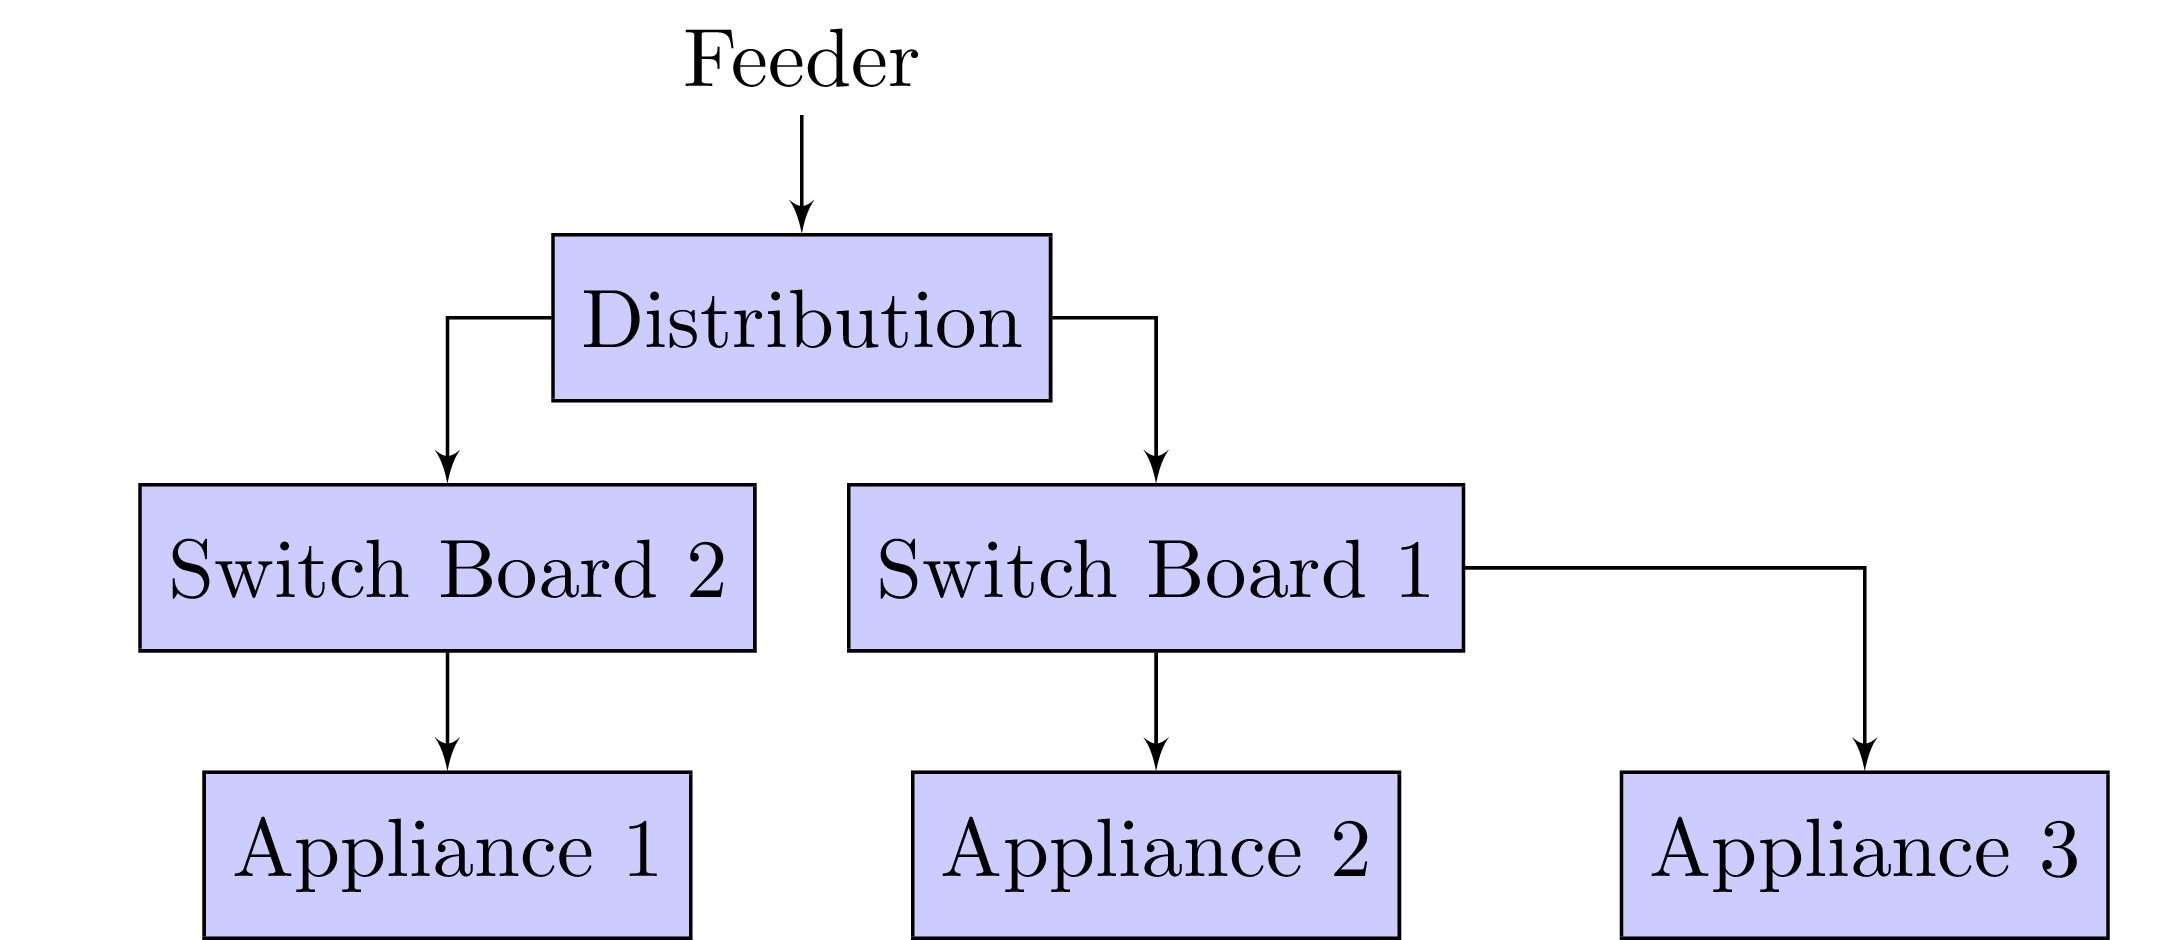
\includegraphics[width=1\linewidth]{tikz/distribution}
	\caption[Distribution of Power]{Distribution of Power}
	\label{fig:distribution}
\end{figure}

\begin{figure} 
	\centering
	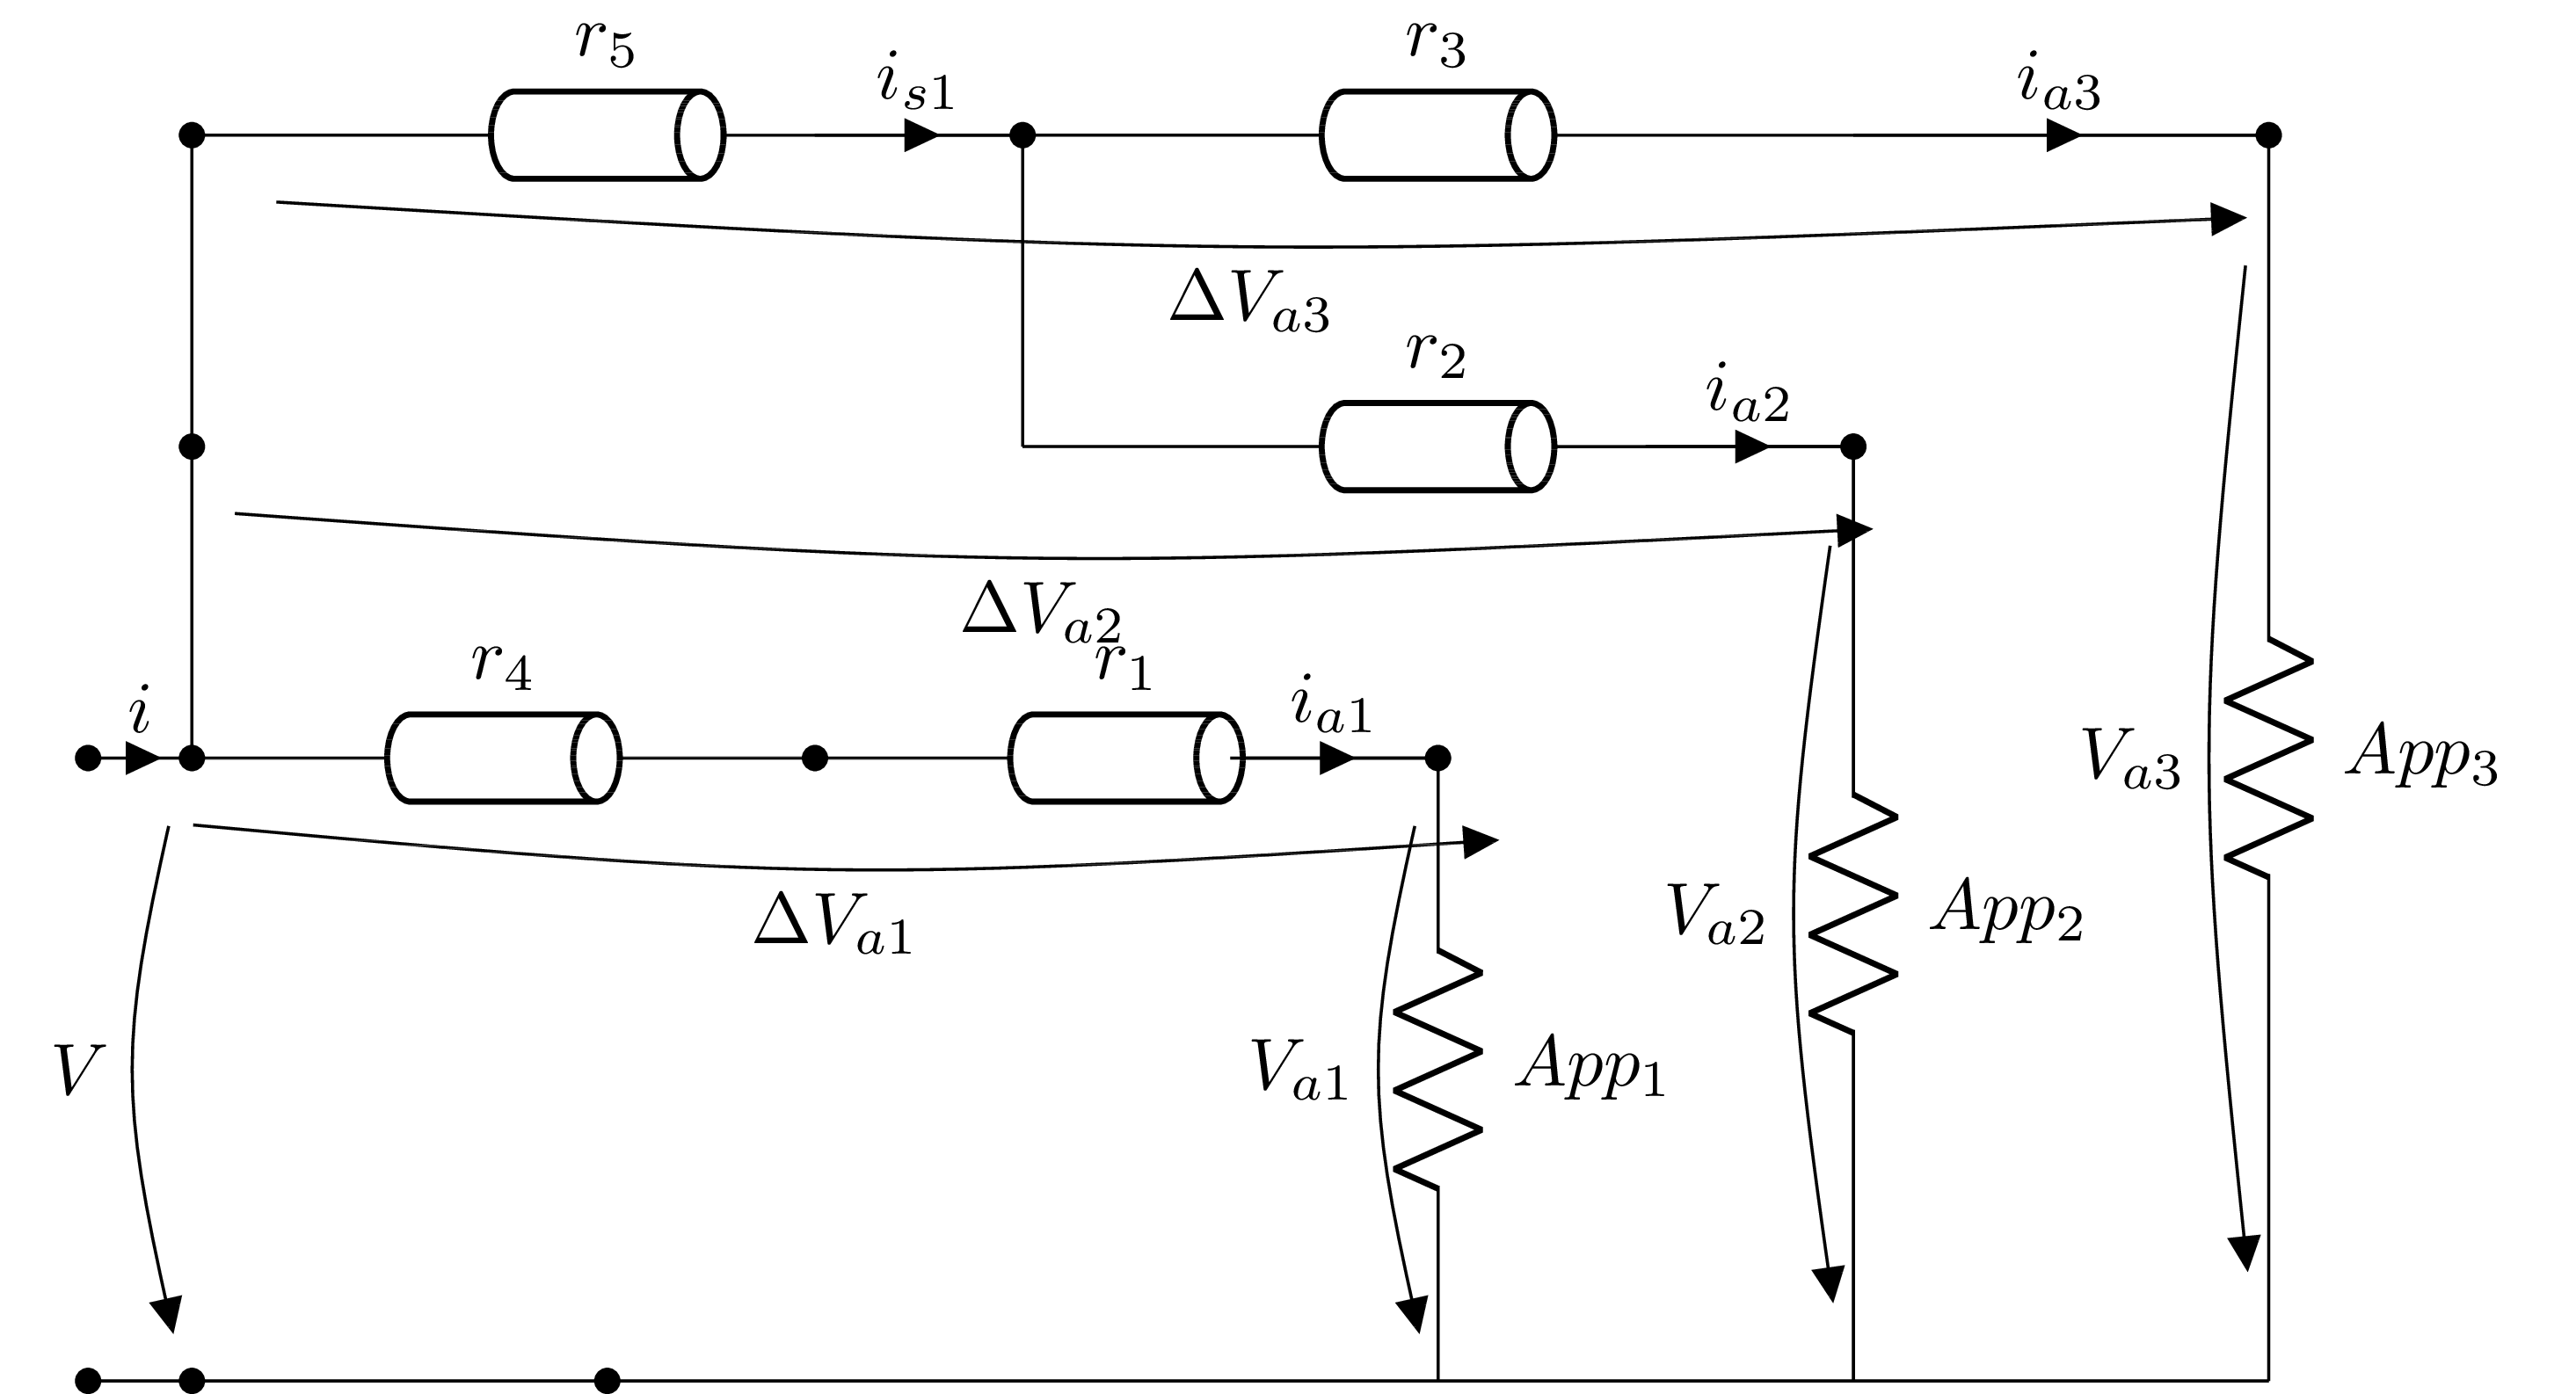
\includegraphics[width=1\linewidth]{tikz/DistributionCircuit}
	\caption[Distribution Circuit]{Distribution Circuit}
	\label{fig:DistributionCircuit}
	\vspace*{-3ex}
\end{figure}

%Conventionally only resistive, inductive and capacitive loads existed. In an alternating supply, the current drawn by the load is also alternating. for a resistive load, the phase of the sinusoidal alternating current is the same as the phase of the supply voltage.  The voltage and current waveform for the resistive types of load is shown in figure [].

%The power drawn by the load is the product of the voltage and current. In the figure [], voltage and the current waveforms are represented by V and I and the power for the resistive load is given by the curve $Power$. It can be observed that power is positive even when the voltage is negative because the sign of the current is always the same as that of the voltage.

In the case of the inductive load, the power is sometimes negative, which indicates outflow of the power from the inductor, when the sign of the current is not the same as the sign of the voltage. In case of a purely inductive load, the sum of the inflow and the outflow of the power is zero. The amount of power absorbed by the inductor is pushed back into the supply in other parts of the cycle.

The ratio of the power consumed by the appliance to the total power flowing through the wire is known as the power factor. The power not consumed by the appliance and pushed back is known as reactive power. Electrical meters can measure reactive power and power factor also.

In reality, most appliance, like electric motors which have inductors or coils consist of some resistive and some inductive component. Hart used both active and reactive power measured at the mains to identify the appliance state. So both the nature of the appliance and the power rating of the appliance are used to identify the appliance.

% for a capacitive load, the current wave leads ahead of the voltage while for an inductive load the current wave lags behind the voltage.

Unfortunately, this approach works only when one of each type of appliance is installed in a house.  It also fails when more than one electrically similar type of appliances are installed in the house like a fan and a motor.

Current can be sensed to determine the power consumed by an appliance. If the power factor of an appliance is assumed to be constant, the power consumed by it can be given in terms of the current drawn by the appliance as 

\begin{equation}
\label{eq:currentValue}
i_a \propto P_a \hspace{.5in} \text{ or } \hspace{0.5in} i_a = \frac{y}{x} P_a 
\end{equation}

%$$ i_a \propto P_a \hspace{.5in}
%or \hspace{0.5in}
%i_a = \frac{y}{x} P_a $$
%\noindent

where $\frac{y}{x}$ is such that when appliance is consuming $x$ power it draws $y$ current. 

 	
In an electrical distribution system, some power is always lost in different stages of delivery.
%Losses can be minimized either by decreasing the wire resistance or by reducing the current.
It is possible to deliver the same power to an appliance by decreasing the current and increasing the voltage by the same factor. This approach is utilized in the long-distance transmission lines where power is transmitted at a very high voltage to minimize these losses. But, a high voltage is not suitable to be used in human proximity because of it's hazardous nature. The only option available is to reduce the power loss is to reduce the resistance of the wire by increasing the diameter.
%, but it can not be done beyond a certain level because of cost and other practical considerations. The lower resistance of the wire can be achieved by increasing the thickness of the wire.
But it can not be done beyond a limit because of the cost consideration. The resistance of the wire can be reduced up to a level beyond which the power loss is not significant enough to justify the increase in the wire cost. In practice, this loss can be in the range of 4-6 \% of the peak load capacity of the line \cite{ElectricalWireGauges}. This can be directly translated to a 4-6 \% drop in the voltage observed at the appliance when operating at its full load.

The second impact of cost consideration is the sharing of a supply line across multiple appliances; this reduces both the cost of installation and power losses. In any common home installation, the power is supplied from the feeder to the house distribution point through a single wire, from where it is connected to different switchboards, from the switchboard a single wire is connected to individual appliances. Such electrical distribution can be represented by a tree structure as in Figure \ref{fig:distribution} where the individual appliances are at the leaf level and the feeder is at the root level.
We will use this as our running example for the rest of the paper.

\begin{table}[htb]
	\centering
	\caption{Power rating of the appliances in the sample circuit}
	\begin{tabular}{@{}lcr@{}}
		Appliance &  Appliance State & Power consumption (Watt) \\
	\midrule
		Appliance 1  &  O  &  0 \\
		Appliance 1  &  A  &  x \\
		Appliance 2  &  O  &  0 \\
		Appliance 2  &  B  &  2x \\
		Appliance 3  &  O  &  0 \\
		Appliance 3  &  A  &  x \\
		Appliance 3  &  B  &  2x \\
	\bottomrule
	\end{tabular}
	\label{tab:powerRatings}
\end{table}

The current flowing through the wire causes a proportional drop in the voltage because of the wire resistance.
This voltage difference $ V_w$ across the wire with resistance $r_w$ is given by
	\begin{equation}
	 V_w = i_a r_w = \frac{P_a}{V} r_w
	\end{equation}
where $P_a$ is the power consumed by the appliance $a$, $V$ is the mains voltage, $i_a$ is the current flowing through the wire. As the resistance of the wire is constant and the mains voltage is always within a short range, the voltage across the wire will be proportional to the appliance power or appliance current.
We measure this voltage across a wire to identify the current flowing through the wire and determine the appliance state.


	The voltage observed across the appliances in the circuit is given by

	\begin{equation}
		\begin{split}
			V_{a1} & = V - V_{r1} - V_{r4}
			= V - r_1 i_{a1} - r_4 i_{a1} \\
			V_{a2} & = V - V_{r2} - V_{r5}
			= V - r_2 i_{a2} - r_5 ( i_{a2} + i_{a3}) \\
			V_{a3} & = V - V_{r2} - V_{r5}
			= V - r_3 i_{a3} - r_5 ( i_{a2} + i_{a3})
		\end{split}
	\end{equation}
	where $V_{r1..r5}$ are the voltages across the wires $r_{1..5}$.
%\textit{It can be observed that the voltage values across appliances 2 and 3 are not only dependent on the current drawn by the appliance itself but also on the appliance that is sharing the line wire somewhere up the supply network. }
Because of the shared resistance $r_5$, both $V_{a2}$ and $V_{a3}$ are dependent on $i_{a2}$ and similarly $V_{a2}$ and $V_{a3}$ are also dependent on $i_{a3}$.
For simplicity, if we assume that all the wires in the setup have the same resistance $r$, that is, they are not dependent on the length of the wires,
the voltage drop for at each appliance is given by the follows equations

	\begin{equation}\label{eq:voltageDrop}
		\begin{split}
			\Delta V_{a1} = & V_{r1} + V_{r4} = r (2 i_{a1}) \\
			\Delta V_{a2} = & V_{r2} + V_{r5} = r (2 i_{a2} + i_{a3}) \\
			\Delta V_{a3} = & V_{r3} + V_{r5} = r ( i_{a2} + 2 i_{a3} )
		\end{split}
	\end{equation}

The voltage observed across a wire is dependent on the current flowing through the wire.
\begin{equation}
\label{eq:voltageeq}
V_r \propto i_a \hspace{0.5in} \text{ or } \hspace{0.5in}V_r = \frac{z}{y} i
\end{equation}
%$$V_r \propto i_a
%\hspace{0.5in} or \hspace{0.5in}
%V_r = \frac{z}{y} i $$
%\noindent
where $\frac{z}{y}$ is such that when $y$ current is flowing through the resistance results in $z$ voltage across the wire.




Voltage sensing requires knowledge of the layout and the connection between different components of the system.
Figure \ref{fig:DistributionCircuit} shows the circuit representation of the home layout shown in the figure \ref{fig:distribution}.
In the circuit, $App_{1} .. App_{3}$ are the appliances and the current drawn by each appliance are given by $i_{a1} .. i_{a3}$. Current for both the appliances appliance 2 and appliance 3 is supplied through the switchboard 1 therefore the current to the switchboard $i_{s1}$ will be the sum of $i_{a1}$ and $i_{a2}$, similarly $i$ is the total current flowing supplied to the system which is the sum of the current for the three appliances.

Resistance of the wires connecting different components is given by $r_{1} .. r_{5}$. The wire represented by $r_{5}$ supplies power to the switchboard 1 from where appliance 2 and appliance 3 are supplied through the wires represented by $r_{2}$ and $r_{3}$ respectively. $V$ is the mains voltage and the V$_{a1} .. V_{a3}$ are the voltage observed across the appliances and $\Delta V_{a1}.. \Delta V_{a3}$ are the differences between the mains voltage and the voltage observed at the respective appliances.


\begin{table}[htb]
	\centering
	\caption{Comparison of disaggregation performance with and without voltage sensing.}
	\begin{tabular}{@{}ccrrr@{}}
		 &  & f-score \\
		Appliance  &  PQ  &  V at App1  &  V at App2  &  V at App3 \\
	\midrule
		1  &  0.4298  &  0.4040  &  0.4129  &  0.4344 \\
		2  &  0.2696  &  0.3138  &  0.7688  &  0.4094 \\
		3  &  0.4889  &  0.4183  &  0.5193  &  0.8818 \\
	\bottomrule
	\end{tabular}
	\label{tab:voltageResult}
\end{table}

\begin{figure} 
	\centering
	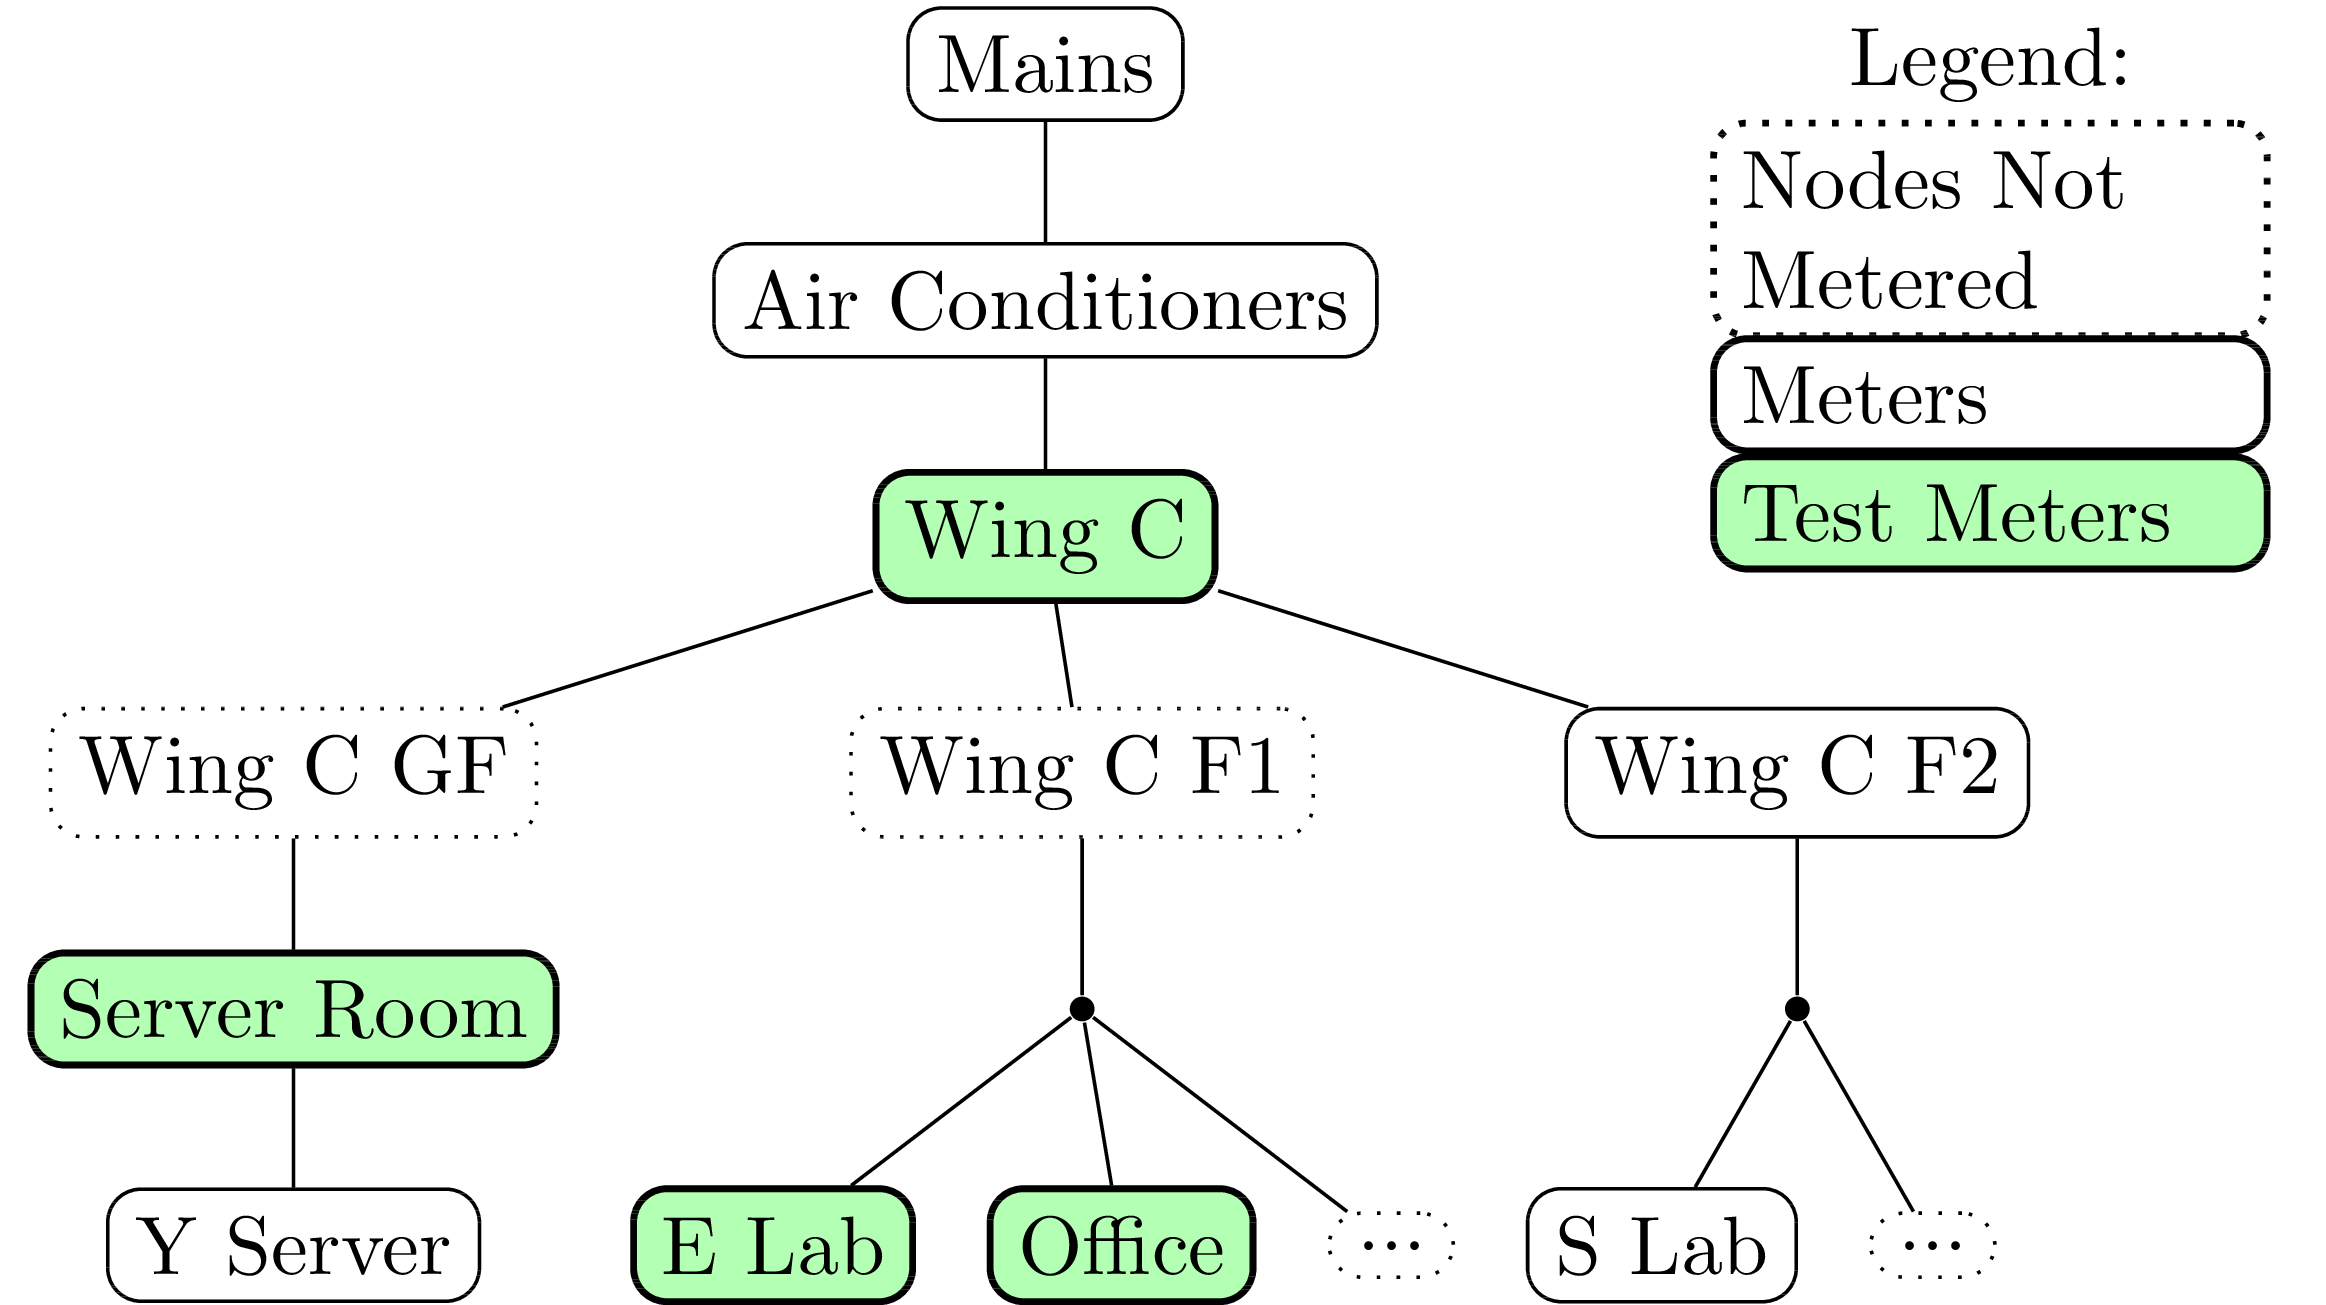
\includegraphics[width=1\linewidth]{tikz/tree}
	\caption[Meters installed in air conditioner line in our academic building]{Meters installed in air conditioner line in our academic building}
	\label{fig:tree}
	\vspace*{-3ex}
\end{figure}

\begin{table}[htb]
	\centering
	\caption{Number of appliance events observed at the target meters during one month period.}
	\begin{tabular}{@{}ccr@{}}
		Meter location  &  Meter type  &  Transition count \\
	\midrule
		Wing C   &  Mains  &  173842 \\
		Server Room   &  Appliance 1  &  21512 \\
		Office   &  Appliance 2  &  202 \\
		E Lab  &  Appliance 3  &  5773 \\
	\bottomrule
	\end{tabular}
	\label{tab:transition}
\end{table}

	
	\chapter{Optimal Sensor Placement}
We now examine the following problem: identifying the number, type, and location of each sensor required for determining all the unique states of the system. A simple approach to make sure to identify all system the states is to install a sensor at each appliance or zone. The number of sensors needed in this case will be equal the number of appliances.

We show now that the objective can be achieved by installing a smaller number of sensors by solving it as a linear optimization problem as follows.

Let there be an electrical system than can be divided into $n$ zones represented by a set $$Z = \{z1, z2, z3 ... zn \}$$. Power consuption of zone can be represented by a set $$P_{zi} = \{p_{z1}.1, p_{z1}.2 ... p_{z1}.m1\}$$. Here zone one can consume one of the $m1$ possible power consumption possible. A zone can consume a power out of a finite number of significant power level. The total number of states in the system will be given by 

\[
|P|  = \prod_{i = 1}^{n} |P_{z1}|  
\]


Our example circuit will have 12 distinct system states, 12 being the product of the number of unique states of each of the appliances.

We define the state of the system by a set of tuples 

$$T = \{(p_1(t), p_2(t),...p_n(t))| p_1(t) \in P_{z1} , p_2(t) \in P_{z2} ... \}$$ 

where each element of the tuple is the power consumed by a zone.

In the system it is possible to install sensors at various places. Let these places be defined by the set $$L = \{l_1, l_2,...l_o\}$$

at these places a number of parameters can be observed. These parameters are represented by a set $$F = \{f_1, f_2,...f_r\}$$

Therefore the possible sensors that can be installed to observe different parameters can be given by set $$S = \{(l_i, f_j)| l_i \in L, f_j \in F\}$$ 

Therefore the number of possible sensors is given by $|S| = |L| * |F|$

Our objection is to select the minimum number sensors that when installed will provide sufficient information to identify the state of the entire system.

In our example, the possible places where the sensors can be installed are 

${Mains, Aplliance 1, Aplliance 2, Aplliance 3, SB 1, SB 2}$
We are selecting only three type of sensors for this example namely 
$$Power, Voltage, Current$$
Here the power is sensed by an smart meter. As a smart meter will also profide voltage and current values, the voltage and a current values provide by the smart meter is but it is not counted as a seperated sensor. It is also assumed that a smart meter is installed by default at the mains. 

The short notations used by different sensors are as follows. Current sensor at switchboard is 
$$i_{s1}$$ 
the current at the appliances are 
$$i_{a1} , i_{a2}i_{a3}$$, 
and the voltage at the appliances are 

$$\Delta V_{a1}, \Delta V_{a2}, \Delta V_{a3}$$

We define a decision variable $u_j$ as
\begin{equation}
u_{j} = \begin{cases} 1,& \text{if sensor } j \text{ is used } \\
0, & \text{otherwise} \end{cases}
\end{equation}
The value sensed by sensor $j$ in system state $i$ is given by $x_{ij}$.
%When the sensor is used, all the values sensed by it will be available for identification of the system state.
The objective is to
$$\min \sum u_j$$
such that we obtain a distinct set of values for the system states, i.e.,
$$|set(x_{ij} * u_j)| = m$$
The problem is NP-hard as all the possible sensor placements should be checked for finding an optimal solution, making the time complexity of searching for the optimal solution, $O(2^n)$.

Although many approaches are available to track appliance operations, most of them are not suitable for office like buildings where a large number of similar appliances are usually installed. All instances of the same appliance are likely to have similar power consumption as well as high-frequency characteristics.
Installing additional sensors is the only option available in such cases. We  present an algorithm for the placement of voltage and current sensors and get full visibility of the state (i.e., ON/OFF) of each appliance in a circuit.

Consider the sample electrical layout, shown in the Figure \ref{fig:distribution}, used to demonstrate our approach.
%rg
The power consumption values of the appliances are selected to point out different desegregation difficulties and explore their solutions.
The power consumed by the three appliances is given in Table \ref{tab:powerRatings}. Appliances 1 and 2 have different power signatures, therefore it is straightforward to disaggregate the consumption if only these two appliances are present. It becomes difficult when overlapping appliance signatures are present, for example, appliances 2 and 3 both can cause an increase of 2x power. Given a transition of 2x Watt increase in power consumption, it will be difficult to determine which appliance is causing it. Some disambiguation can be achieved if the state from which the transition occurs is also included in the decision making, For example if the system is in state O,O,A and a 2x increase in power is observed, it can only because of appliance 2, but not all instances of the problem can be resolved using such information.

For example, when the power consumption increases by x Watt, it may not be possible to determine whether the increase is because of appliance 1 or appliance 3.
%kk  3,  not 1, no? yes
Figure \ref{fig:sys} shows all the possible states of the system based on the state of each appliance and possible change of appliance states when only one appliance is changing its state.
Each state in the diagram is associated with a tuple, ($A,O,B$), where \textit{A, O} and \textit{B} respectively representing the state of the three appliances: appliance 1 is in state $A$ consuming x Watt, appliance 2 is in state $O$ consuming 0 Watt, and appliance 3 is in state $B$ consuming 2x Watt power. If the power consumption of the system decreases by x Watt, the next possible state of the system can be ($O,O,B$) or ($A,O,A$). Such non-deterministic transitions are shown by dotted lines in this figure.
In such a situation, a probabilistic model can be used which utilizes other information like appliance behavior to resolve such confusion. For example, if appliance 1 is a bulb it is less probable to be switched ON at day and more probable to be switched ON at night. Appliances like Air conditioners consume power in cycles. The time period of the ON-OFF cycles of such appliances can also be used to identify their operation. The probability of use of different appliances will be different at different times. The probabilistic algorithm can utilize this probability to identify the correct appliance. But with a large number of appliances with  similar probability, such algorithms will not give accurate results.

\begin{figure} 
	\centering
	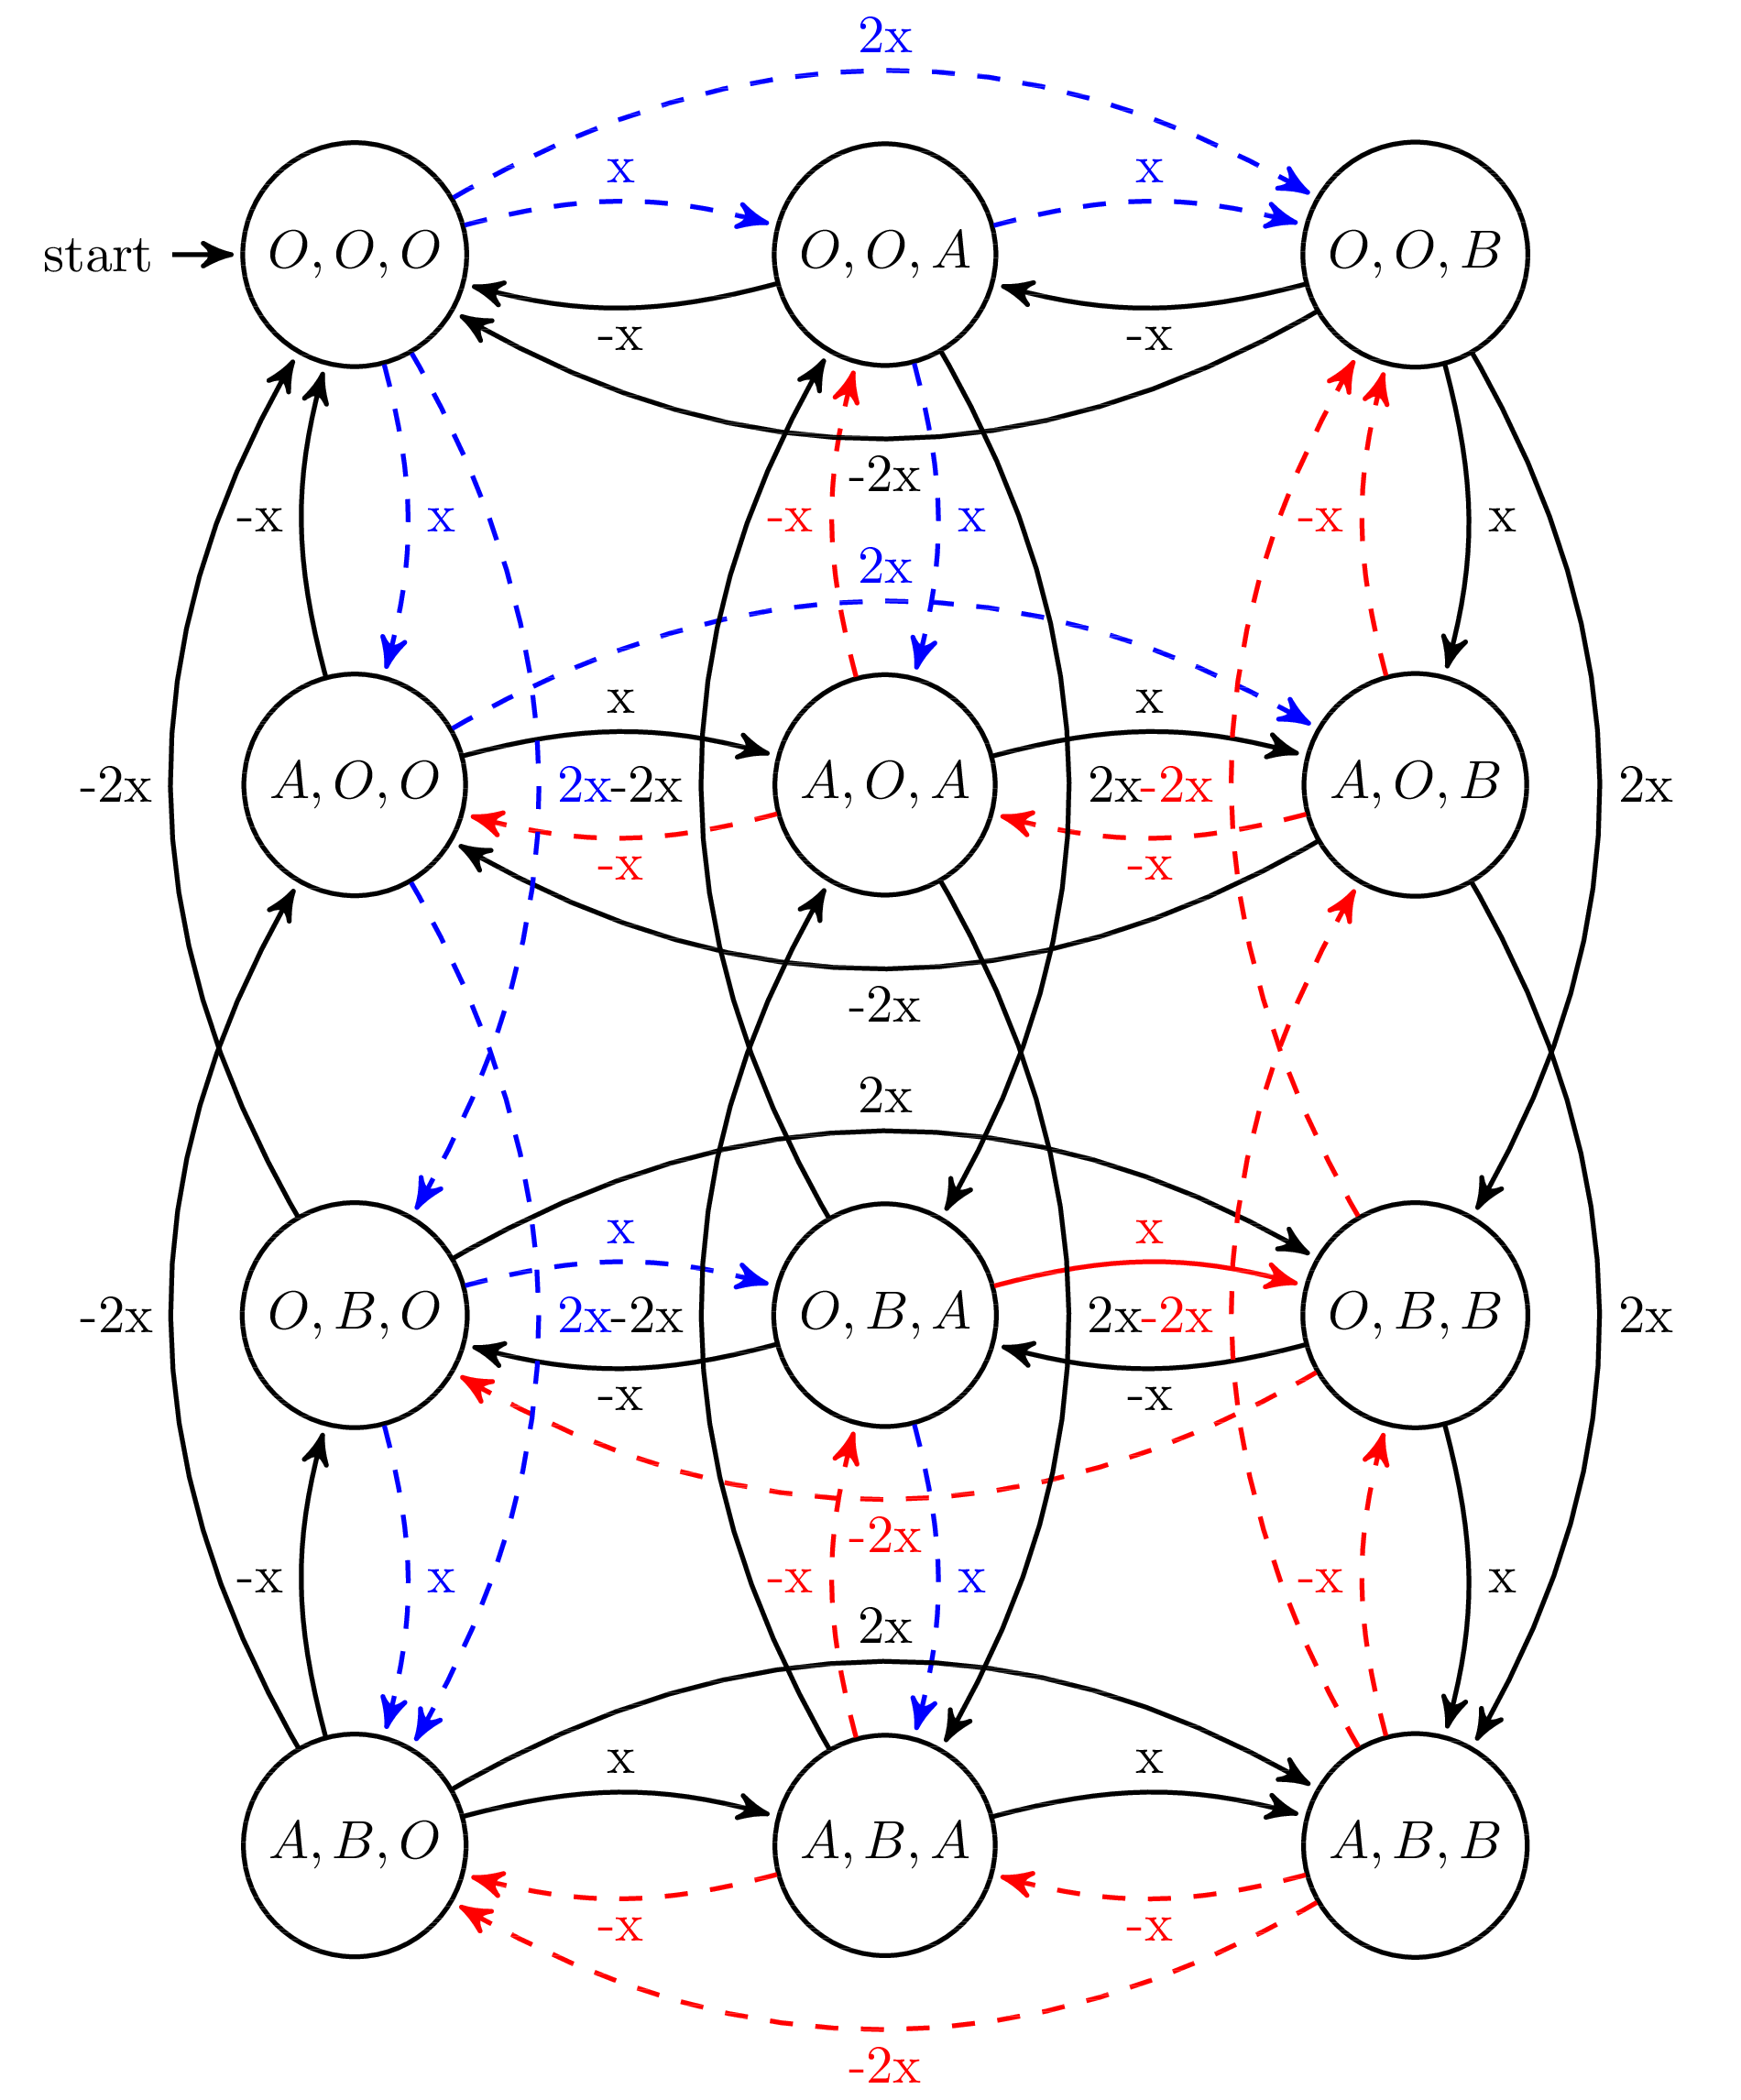
\includegraphics[width=1\linewidth]{tikz/sys}
	\caption[State transitions for the sample circuit]{State transitions for the sample circuit}
	\label{fig:sys}
	\vspace*{-3ex}
\end{figure}

Our algorithm adopts a greedy approach. %which provide a solution in between the two extremes.
The input to the algorithm is a table consisting of all the values for $x_{ij}$
where each row represents a system state, and each column represents a sensor.
It adds one sensor at a time such that, when added, it produces the largest increase in the set of distinct sensed values.

The values in the table \ref{tab:sensorTable} for the sample layout are constructed as follows:
Columns ${P_{a1..a3}}$ are the appliance level power values based on the table \ref{tab:sensorTable}. For this running example, the appliance power values are used to assign the values sensed by different sensors. The smart meter installed at the mains $S_{PMains}$ will sense the total power consumption which is the sum of the power consumed by all the appliances. The current sensors $S_{ia1..ia3}$ can be installed at the individual appliances.

Values that would be sensed by the current sensors is given by appliance power and equation \ref{eq:currentValue}. For example, for the state (O,B,A) the power consumption for appliance 1, 2 and 3 will be $0$, $2x$ and $x$ Watts respectively.
The current drawn by these appliances will be $0$, $2y$ and $y$ respectively, for some $y$.
Current sensors can also be installed at the switchboard to sense the total current consumed by the appliances supplied through the switchboard. Sensor $S_{s1}$ installed at the \textit{switchboard 1} will observe the sum of $i_{a2}$ and $i_{a3}$.

Values for voltage sensors $S_{\Delta V1..\Delta V3}$, installed to sense the voltage drop at respective appliance, can be computed using the equations \ref{eq:voltageeq} and \ref{eq:voltageDrop}.
for example for the state (O,B,A) the current drawn by the appliances will be 0, 2y and y respectively, thus voltage drops at each appliance will be 0, 5z and 4z respectively.


In Algorithm \ref{alg1}, ($T$) is the table that has the set of sensors ($S$) already installed in the system and $h$ the desired maximum number of sensors.
The variable $S_{sel}$ holds the currently selected set of sensors, and $T_{sel}$ the projected part of the table consisting only of selected columns. The set of sensors finally chosen for installation is returned in ($S_{sel}$).  Function $Project$  accepts two parameters, $T$, a table containing the values sensed and a set of sensors $S_{sel}$ and returns the table consisting of the columns for the sensor set $S_{sel}$.
Function $set$  returns the distinct tuples from the given table.

Initially, the list of sensors already installed will be just the mains meter that is $S = [S_{PMains}]$.
$S_{PMains}$ is the power measured by the mains meter.
In each iteration, $argmax$ will select a sensor which when added to the existing list $S_{sel}$ will result in a new projected table $T_{sel}$ with the maximum number of unique rows.
For example, when only mains meter is installed, only $S_{PMains}$ will be projected in $T_{sel}$.
The set of distinct values in the columns listed  in $T_{sel}$ will be $\{0,x,2x,3x,4x,5x\}$ and the size of the set will be 6.

Suppose $S_{ia1}$ is also added to $S_{sel}$ the distinct values in $T_{sel}$ will be $\{(0,0),(x,0),$ $ (2x,0),(3x,0),(4x,0),$ $ (x,y),(2x,y),(3x,y),$
$(4x,y),$ $(5x,y)\}$ and its size of the set will be 10.
But, suppose we add $S_{ia3}$
 $T_{sel}$ will be maximum (12): $\{(0,0), (x,y), (2x,2y),$ $ (2x,0),$ $ (3x,y),$ $ (4x,2y),$ $ (x,0),$ $(2x,y),$ $ (3x,2y),$ $ (3x,0),$ $(4x,y),$ $ (5x,2y)\}$.
 Alternatively, if  we choose  $S_{\Delta Va2}$ ,
 the size of $T_{sel}$ will also be 12: $\{(0,0),$ $(x,z),$ $ (2x,2z),$ $ (2x,4z),$ $(3x,5z),$ $(4x,6z),$ $(x,0),$ $(2x,z),$ $(3x,2z),$ \\$(3x,4z),(4x,5z),(5x,6z)\}$.

Thus, the number of rows will be equal to the total number of states when either $S_{PMains}$ with $S_{ia3}$ or $S_{PMains}$ with $S_{\Delta Va3}$ are installed. Therefore the algorithm will return one of these two pairs of sensors.
%r
% \textbf{Added Text}

When current sensors are installed close to the appliances to monitor each appliance, the number of sensors required will be equal to the number of appliances. Following placement algorithm will provide a solution which will produce the same result with significantly less number of sensors.

The Greedy algorithm not only provides a solution to the sensor placement problem, but it also enables us to incrementally install sensors while maximizing the system observability with the given number of sensors. In a building where smart meters are already installed the voltage readings provided by the meters can improve the disaggregation output without installing any other additional hardware. Even when all the appliances are monitored by power meters, voltage sensing can be used as a backup mechanism when some of the sensors fail.

We will prove that \textit{Subset Cover} can be reduced to \textit{Sensor Selection} problem in polynomial time. Therefore the \textit{Sensor Selection} problem is at least as hard as \textit{Subset Cover} problem.

    \textbf{Subset Cover Problem}

Given a family of sets $E$ and a universe $U$ where $\cup E = U$, the objective is to find the smallest set of sets $C$, such that $C \subset E$ and $\cup C = U$.

	\textbf{Sensor Selection problem}

Given an electrical system which can be in one of the states in set $T$, and a set of sensors $S$. Each sensor when installed will sense values given by set of values $Q$ such that
\begin{equation} \label{eq:reduction1}
|Q|>1
\end{equation}

Our objective is to find out the minimum number of sensors which when installed will provide tuple of sensed values each state, given by matrix $R$ such that the sensed values are unique for each state.

\begin{equation} \label{eq:reduction2}
\forall q,r \in R, q \ne r
\end{equation}

Each sensor will sense some value for each sensor state and the distinct values sensed by a sensor should be more than one else it will not contribute to the uniqueness of the sensed values.

\textbf{Reduction Function }

For problem translation we will map each set to a sensor and each element of the set $U$ to a state in the electrical system. The value sensed by a sensor in a state will be given by the index value of the set element in $U$.
%rg
To meet the condition given in the equation \ref{eq:reduction1}, we define a new element $e_0 \notin U$, and add it to each set.
% rg end
Therefore sets $U_1 = U + e_0$  and $E_1 = E + e_0$.

The reduction function will construct a table with values using following equation.

\begin{equation*}
u_{ij} = \begin{cases}    index(e_j),& \text{ if } e_j \in E \\    0,& \text{otherwise} \end{cases}
\end{equation*}

As translation will be required for each sensor and state in the system, the complexity of the function is $O(mn)$.

\textbf{Validation Function}

A polynomial time function is required to validate if the given set of sensors is a valid solution of the problem. This function will check if $|U_1| == |T_s|$. Unique elements in a list of values can found out in linear time by using a hash function. Therefore the time complexity of the validation function will be $O(n)$.

\textbf{Translation of the Solution}

The set of sensors selected by the algorithm will be the same as the set of subsets i.e. $C = S$, Therefore no translation will be required for the solution.

\subsection{Greedy algorithm}
\begin{figure} 
	\centering
	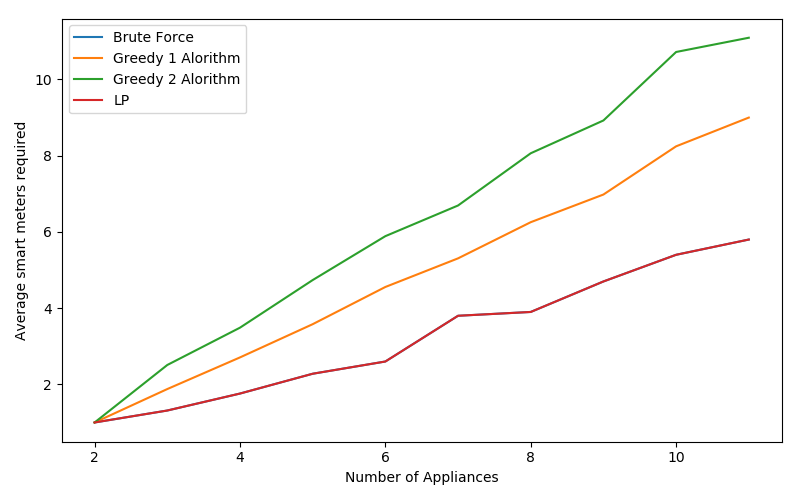
\includegraphics[width=1\linewidth]{images/optsens}
	\caption[Number of smart meter requirement given by different algorithms]{Number of smart meter requirement given by different algorithms}
	\label{fig:optsens}
	\vspace*{-3ex}
\end{figure}

\begin{figure} 
	\centering
	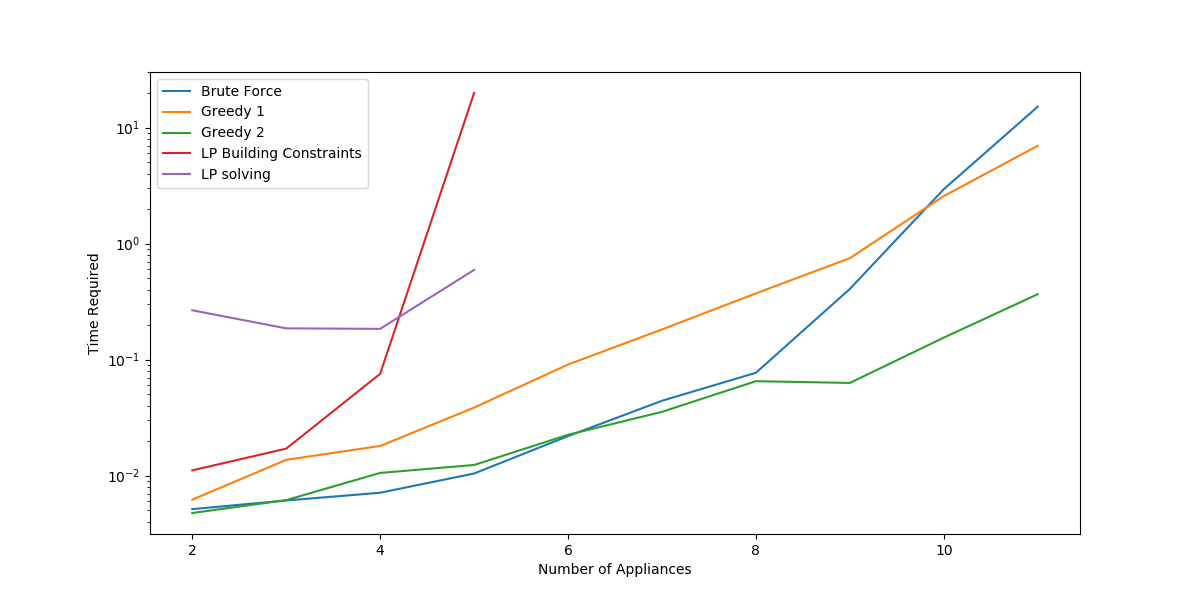
\includegraphics[width=1\linewidth]{images/opttime}
	\caption[Time required by different algorithm]{Time required by different algorithm}
	\label{fig:opttime}
	\vspace*{-3ex}
\end{figure}

\begin{figure} 
	\centering
	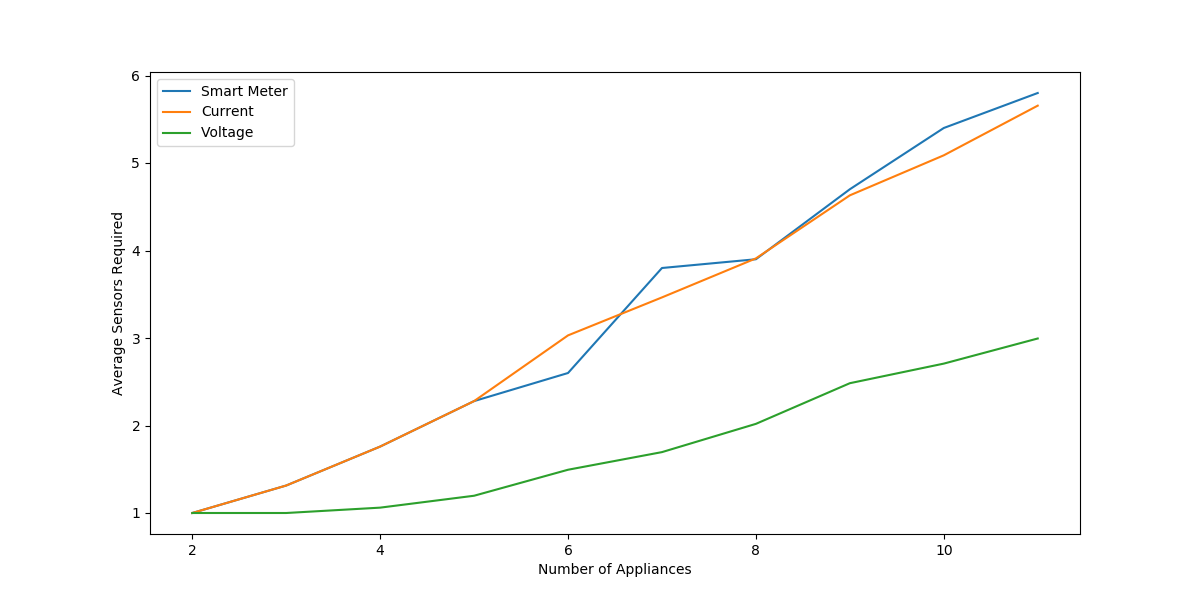
\includegraphics[width=1\linewidth]{images/sensreq}
	\caption[Relative Smart mete, Current sensors and Voltage sensors requirement]{Relative Smart mete, Current sensors and Voltage sensors requirement}
	\label{fig:sensreq}
	\vspace*{-3ex}
\end{figure}

\begin{figure} 
	\centering
	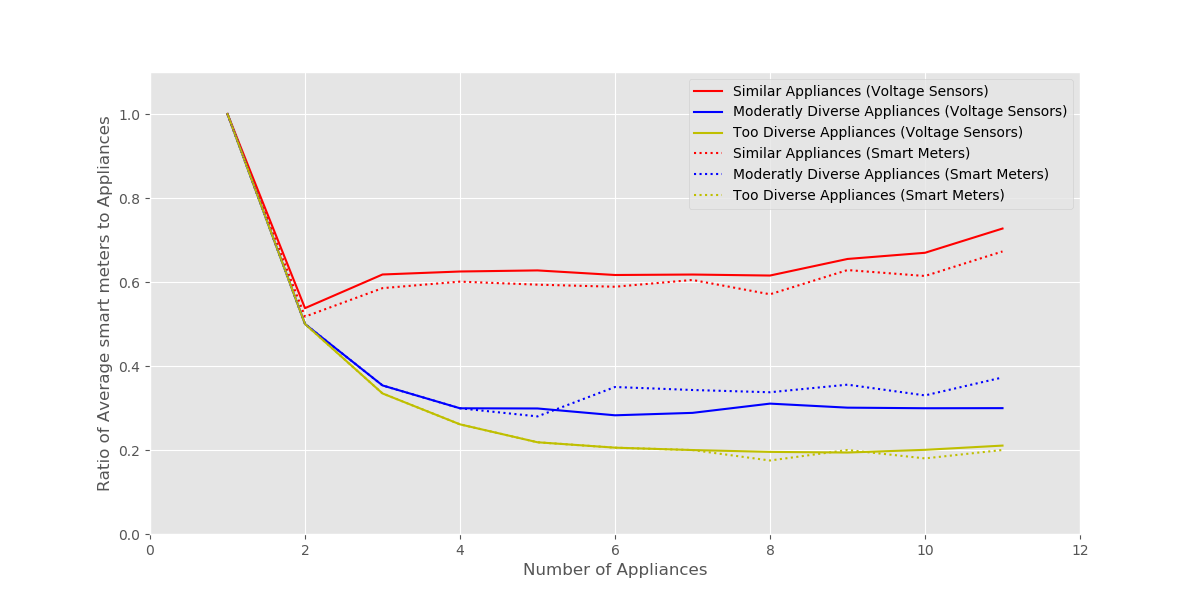
\includegraphics[width=1\linewidth]{images/sim_V_b}
	\caption[Number of smart meters required relative to number of appliances installed]{Number of smart meters required relative to number of appliances installed}
	\label{fig:sim_V_b}
	\vspace*{-3ex}
\end{figure}

\begin{algorithm}
	\caption{Greedy algorithm for sensor placement}
	\label{algo:greedyalgorithm}
	\textbf{Input:} T, S, h
	\begin{algorithmic}
		\State $S_{sel} \gets S$
		\While{1}
		\State $T_{sel} \gets Project (T,S_{sel} ) $
		\If {$|set(T_{sel})| == |T| \textrm{ or } |set(T_{sel})|==h$}
		\Return $S_{sel}$
		\EndIf
		\State $ s \gets \argmaxl_{s\notin {S_{sel}}} |set(Project(T,S_{sel} + s))|$
		\State $ S_{sel} \gets S_{sel} + s$
		\EndWhile
	\end{algorithmic}
\end{algorithm}

\begin{table}[htb]
	\centering
	\caption{Power, Current and Voltage difference sensed by all possible sensors for all possible states (load combinations) of the Appliances.}
	\begin{tabular}{@{}cccccccccccc@{}}
		State  &  $P_{a1}$  &  $P_{a2}$   &  $P_{a3}$   &  $S_{PMains}$  &  $S_{ia1}$  &  $S_{ia2}$   &  $S_{ia3}$   &  $S_{s1}$   &  $ S_{\Delta Va1}$  &  $S_{\Delta Va2}$  &  $S_{\Delta V a3}$ \\
	\midrule
		OOO  &  0  &   0  &   0  &  \cellcolor{green!20}0  &  0  &   0  &   0  &   0  &   0  &   0  &   0 \\
		OOA  &  0  &   0  &   x  &  \cellcolor{green!20}x  &  0  &   0  &   y  &   y  &   0  &   z  &  2z \\
		OOB  &  0  &   0  &  2x  &  \cellcolor{green!20}2x  &  0  &   0  &  2y  &  2y  &   0  &  2z  &  4z \\
		OBO  &  0  &  2x  &   0  &  \cellcolor{green!20}2x  &  0  &  2y  &   0  &  2y  &   0  &  4z  &  2z \\
		OBA  &  0  &  2x  &   x  &  \cellcolor{green!20}3x  &  0  &  2y  &   y  &  3y  &   0  &  5z  &  4z \\
		OBB  &  0  &  2x  &  2x  &  \cellcolor{green!20}4x  &  0  &  2y  &  2y  &  4y  &   0  &  6z  &  6z \\
		AOO  &  x  &   0  &   0  &  \cellcolor{green!20}x  &  y  &   0  &   0  &   0  &  2z  &   0  &   0 \\
		AOA  &  x  &   0  &   x  &  \cellcolor{green!20}2x  &  y  &   0  &   y  &   y  &  2z  &   z  &  2z \\
		AOB  &  x  &   0  &  2x  &  \cellcolor{green!20}3x  &  y  &   0  &  2y  &  2y  &  2z  &  2z  &  4z \\
		ABO  &  x  &  2x  &   0  &  \cellcolor{green!20}3x  &  y  &  2y  &   0  &  2y  &  2z  &  4z  &  2z \\
		ABA  &  x  &  2x  &   x  &  \cellcolor{green!20}4x  &  y  &  2y  &   y  &  3y  &  2z  &  5z  &  4z \\
		ABB  &  x  &  2x  &  2x  &  \cellcolor{green!20}5x  &  y  &  2y  &  2y  &  4y  &  4z  &  6z  &  6z \\
		Rows &   &   &   &   &   10  &  8   &  12    &   10    &   10     &   12     &   10 \\
	\bottomrule
	\end{tabular}
	\label{tab:sensorTable}
\end{table}

In order to evaluate the performance of different algorithms to find the optimal placement of the sensors, and to evaluate the number of each type of sensor required, tests were conducted on a large number of electrical layouts which were generated by using a variety of appliances. Following three types of layouts were generated

\begin{itemize}
    \item Type 1: Mostly similar appliance
    \item Type 2: Moderately diverse appliances
    \item Type 3: Highly diverse appliances
\end{itemize}

For the generation of the $type 1$ layouts, the number of allowed appliances were restricted to a few (2-3) depending on the size of the layout. The selection of the appliance for the $type 1$ layout was such that the power consumption of the appliances was identical for some of the states. Selecting power consumption in this way result in same power consumption for multiple states of the system and a large number of confusions are observed in the system states. For the $type 2$ layouts, the number of the allowed appliance was increased in the range of A1-A2 and for generating the $type 3$  layouts the number of allowed appliance were further increased.

For all the layouts, the length of the wire from the distribution boards to the switchboards and from switchboards to the appliances was taken in the range of $10-50$ meters, and the number of appliances connected to the switchboard was taken in the range of $2-8$ which are the commonly observed parameters in any electrical layout.  Multiple level of the switchboards were also allowed.

The total power consumption for all the appliances under a switchboard was used to identify the current rating and gauge of the wire to connect the switchboard to the distribution board. The wire of  higher diameter (lower gauge) than the recommended current consumption were used.   The electrical parameters of the copper wire for the selected gauge and the length of the wire were used to compute the resistance of the wire and the expected voltage drop at the appliance and the distribution board.


\subsection{Performance of Optimal Sensor Placement}
The default sensor for energy measurement is the smart meter because it is the only sensor which directly provides the power consumed. In the following analysis, we studied the number of smart metes required to identify the state of all the appliances. Our simulations show that the number of smart meters required is directly proportional to the number of appliances installed. The analysis of the diversity of the appliances revels that the number of smart meters required is dependent on the diverse nature of the appliances. If the installed appliances are of similar or identical electrical nature, then the number of sensors required is very near to the total number of the installed appliances, but if the power consumption of the installed appliances is diverse, then the number of meters required can be much lower.

Figure \ref{fig:optsens} shows that the number of smart meters required increases with the appliance installed. Initially the ratio of the number of the smart meters to the number of appliance decreases, this is because the number of sensors required when only one appliance is installed could not be less than one. As the number of appliance increases the ratio decreases and becomes constant. It can be observed in the figure \ref{fig:sim_V_b} that when number of appliances is above 4 this ratio remains constant. This behavior is same for all types of the layouts. In the case of the $type 2$ layouts the number of smart meters required is around 60\% of the number of appliances installed. Therefore we can assume that merely using the algorithm to strategically install the smart meters, the number of smart meter requirement can be reduced by 40\%.

In this strategy, similar to installing the current sensors, only one smart meter is installed at the mains and voltage sensors are installed at all other places. Instead of using the smart meter if the voltage sensor  are installed to detect the drop in the voltage, the number of sensors required is similar to the number of smart meters. Our understanding for this observation is because the smart meters (after installing the mains smart meter) are not adding much information by providing the power measurement. Therefore the only additional information obtained from the meters is the voltage droop.

For the $type 2$ load, the number of sensors required is slightly higher than the smart meter with voltage inference, but it is significantly less than the number of smart meters required when the voltage inference is not used.

Therefore  the number of sensors required for this case
    $$O_P \le  O_V$$
 Overall the cost of the voltage sensor is much less than the smart metre

 Although the number of sensor is almost similar the cost of sensors is much less


In this analysis, current sensors were used at all the places except for the mains meter. The simulation results show that the number of the current sensors required is identical to the requirement of the smart meters. This is because the power measured by the smart meter is mostly dependent on the current drawn by the appliance. The current sensor may perform poorly only in the case when more than one appliance draws the same current, but have different active and reactive power. In our simulations, we have not used appliances of this nature. Because of this property, a large number of products use them instead of smart meter thereby reducing the complexity of the sensor and the cost of the sensor itself. This also reduces the installation complexity if the clamp-on type of sensor is used.

The key point to be noted that the current sensor can never outperform the number of smart meter requirement.
that is $$O_W \le O_C$$

Prior to this work, the voltage sensed by the smart meter is not used for any purpose at all. Based on the technique proposed by us, the voltage sensed by the smart meter can be used to identify the state of the nearby appliances. When smart meters are installed at locations where the voltage sensed by the meter can be utilized to identify the appliance state the number of meters requirement can be reduced.

Figure \ref{fig:sensreq} shows that the number of smart meters required grows proportional to the number of appliances, but the rate of increase is lower when compared when smart meters are used for the power measurement only. The reduction in the number of smart meters is higher in this case and can be up to 30-40\% for $type 1$ layouts. For the moderately diverse appliances ( $type 2$ layouts), the number of smart meter requirement can be reduced by 60\% to that of the total number of appliance installed.  This can be observed in the results shown in figure \ref{fig:sensreq}. As the inference made by the  voltage can only reduce the number of the smart meters, the relative number of sensors required will be less than the number of meters required $$O_P \le  O_W \le  O_C$$

The problem of the identification of the sensor requirement is Np-Hard.  In order to compare the performance of different algorithm we ran the different algorithms for the same set of layouts and compared the number of sensor requirement and the time taken by the algorithm to for find the sensors required.

The number of the system state is the Cartesian product of the individual appliance state. Let $h$ be the average number of state for the appliances, and $m$ be the number of appliances. The number of system states is of the order of $O(h^m)$. To check if the sensed values are distinct the values sensed for each state should be compared at least once. Therefore the time complexity of checking one column in the sensor values table will be $O(h^m)$. The sensor table will consist of $n$ columns where $n$ is the number of possible sensors. For finding the optimal placement using brute force algorithm first each column is checked individually than all the combination of two columns are checked and it is continued till a suitable placement is found. So the number of iterations required is:
$$^ nC_1 + ^nC_2 + ^nC_3 ...  = 2^n $$
Therefore in the worst case the total number of operations required for finding the optimal by brute force in $O(h^m * 2^n)$. assuming that any appliance will have at least two states, $h$ will be $2$ in the best case.  Also as any electrical parameter can be measures at each appliance the number of possible sensors will be at least equal to the number of the appliances installed. Therefore, in the best case, the time complicity for finding the optimal by brute force will be  $O({(2^n})^2)$. for just 16 appliances the required operation will be more than a billion. In our simulations the time required for finding the optimal in such case was  several hours. As the number of appliance in any household may be much higher than 16, algorithm is impractical for regular use.

The brute force algorithm will always provide the optimal solution for the problem but is costly because each combination of the sensor should be checked. When the appliances are diverse, the number of sensor requirement is very low and the algorithm can find out the optimal placement in relatively less time. The sensor requirement increases when the appliances are less diverse and will be very high if all the appliances installed are identical in power consumption. When the diversity of the appliance is less, the brute force algorithm takes longer to find the optimal solution. Figure \ref{fig:opttime} shows that the time required for finding the optimal increases exponentially for all types of layouts but it grows slowly for the type 2 and type 3 layouts.

Almost similar performance is observed irrespective of the type of the sensors selection.

The G1 algorithm tries to maximize the number of states it can identify in each iteration. In each iteration the algorithm check the combination of the already selected sensors with each of the remaining sensors. Therefore the number of iterations performed by this algorithm are
$$ n  + (n-10  + ( n-2)  ... 1 = \frac{(n +1) * n }{2}$$
So the time complexity of this algorithm is  $O(n^2)$.
In the figure \ref{fig:opttime} it can be observed that the time requirements for the the greedy algorithm is linear on the logarithmic scale where the time required for the brute force algorithm grows exponentially on the same scale.

The number of sensors identified by the greedy 1 algorithm is almost same for the $type 2$ and $type 3$ layouts, for the $type 1$ layouts also the number of sensors required is very slightly more than the optimal number of sensors.

The $greedy 2$ algorithm sorts the sensors on the basis of the there individual performance and adds them in the descending order till all the states in the system can be distinctly unidentified in the system. Therefore the time required in identifying the sensor placement is least for the greedy 2 algorithm in least but the number of sensors outputted by the this algorithm is very high which makes this algorithm less useful. In some cases the greedy 2 algorithm performed even worst than the baseline of installing sensor at all the appliances.

The linear programming optimization problem is formulated as a graph cover problem with the additional constraint for each sensor. The graph cover problem formulation itself generate a huge number of constraints, therefore, the constraints for the sensor placement problem are even more.  The number of constraints is larger than the number of interactions performed by the brute force algorithm. Out of these constraints, a huge number of constraints are redundant because the same constraint will be derived from the multiple trees generated by the same sensors.  Because of this reason, the model generation for the electrical layout takes exponentially large time and become impossible to manage just after 4 or 5 appliances. Also, the memory requirement for the model exceeds the RAM available on the standard PC.  Because of these reasons the optimization testing is included up to 4 appliances.

The baseline case of installing the smart meter for each appliance is generally very high. The cost of the Schneider meters is in the around 9000 Rs, For simplicity we will Ignore the installation cost and the cost of accessories.  If such  a meter is installed for every appliance in an electrical system where 12 appliances are installed, the total cost of installing 12 smart meters will be 108000 Rs. Assuming that the appliances are moderately diverse, the cost of the sensor equipment required when the new low cost smart meter is installed will be 6500 Rs. The new cost is just above  6\% of the baseline cost, which gives us more than 93\% reduction of sensor equipment requirements.


	\chapter{Smart Meter}
\begin{figure} 
	\centering
	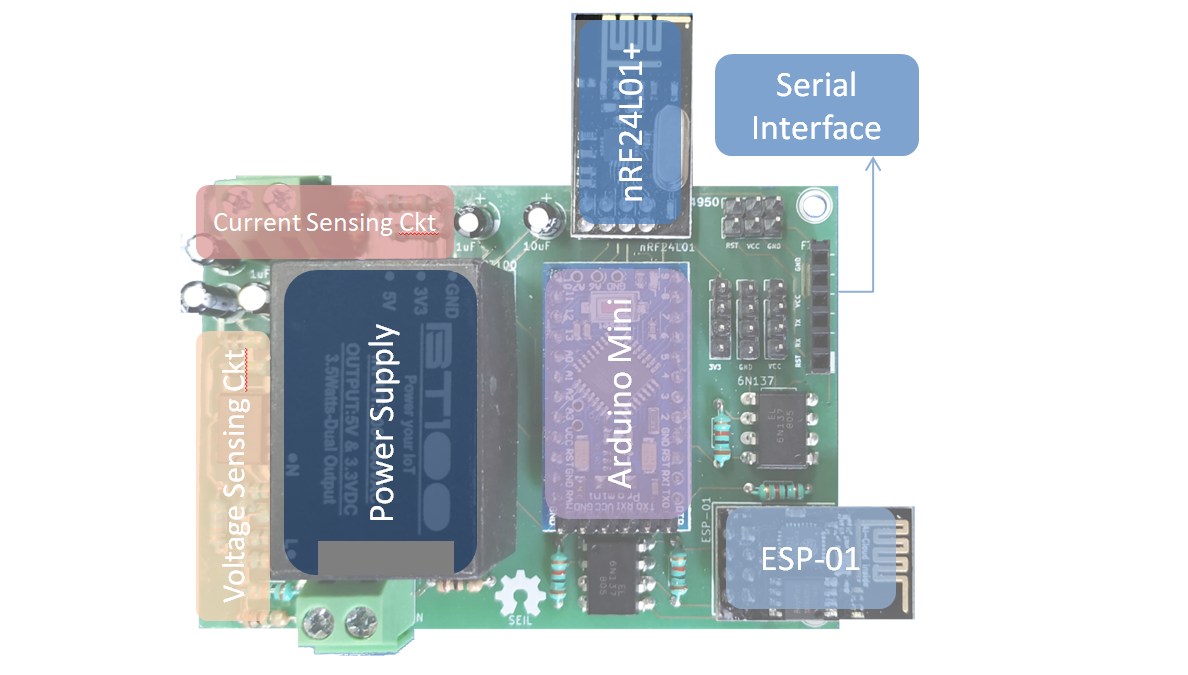
\includegraphics[width=0.8\linewidth]{images/smartmetertagged2}
	\caption[Smart Meter]{Smart Meter}
	\label{fig:smartmetertagged2}
	\vspace*{-3ex}
\end{figure}

Smart meters are the key infrastructure required for the implementation of smart grids that can enable the realization of tasks like demand response, efficient power quality management and sharing of resources like battery and solar PV. Existing smart meters are designed for the purpose of collecting energy consumption data only. These meters will not be able to meet the new requirements arising from the smart grid implementation. Considering these changes in the smart grid, the smart meter should be a combination of modular and upgradeable hardware and software. It should also enable researchers to collect data in the desired way. To enable exponential growth in the metering infrastructure, the following capabilities are desirable.
`
% Task performed by smart meters include tasks like state-of-the-art measurement and calculation, hardware calibration, and communication.

%Knowledge of peak or off-peak periods, energy usage patterns, two-way communication between end-user and utilities is beneficial for utilities. Metering through smart meters in a smart grid can provide these abilities, but methods to implement these capabilities are limited today. Smart meters include measurement and calculation section, hardware and software calibration, and communication capabilities. However, current industrial and research purpose meters fail to adapt to the ever-changing technology. They do not provide enough analytics to observe and understand the usage patterns. Also, they are costly and bulky in design and hence, still less prevalent in developing countries like India.


\subsection{Upgradability}
A smart meter should be \textbf{easily upgradeable} both in terms of hardware and software. Current metering infrastructure has lasted for decades but due to consistently changing requirements of the smart grid, the new smart meters may need to be upgraded more frequently. It is impossible to predict the future requirement accurately and design a smart meter that considers all such future requirements. Hence, the new generation of smart meters must be customizable according to the changing needs to avoid design and development cost and to speed up the development process. Once a smart meter is installed, new analytics and value-added services may be introduced based on the new capabilities of such smart meters. In turn, these services will need more sophisticated meters thereby introducing the update cycle. Therefore, to accommodate the ever-changing software and hardware demands, the new smart meters must be modular and support improvement in each module.


\subsection{Reducing Communication}
The data collected by the smart meter should be \textbf{communicated efficiently and timely} to the server for processing. Two-way communication is one of the important capabilities of smart energy meters. Retrofitting the required communication capabilities to the existing meters is not always possible and may not provide a cost-effective solution. It may not provide sufficient data samples and can make the infrastructure bulky. It also requires a large number of the messages to be transferred which imposes a restriction on the number of smart meters that can be connected on a single communication channel. Therefore a smart meter should provide intelligent inbuilt communication capabilities.



\subsection{Energy Disaggregation}
Smart meters should be able to \textbf{disaggregate energy consumption} and estimate appliance health. The research community has been working on disaggregation since Hart \cite{hartNonintrusiveApplianceLoad1992} and developed a large number of techniques to disaggregate energy consumption.  Disaggregation algorithms need a variety of data like the high-frequency current, voltage for sensing EMI noise or combination of both in VI-Trajectory. All such techniques need data at a very high frequency,  Research is mostly done on the data collected by high-end equipment or data collected from industry-grade meters. These equipment are not suitable for mass deployment, therefore, not practical to be used for large scale installation.  Although almost all meters sense and process the high-frequency data, they only provide the low-frequency electrical parameters computed from the high-frequency data. They do not provide the data as desired by the algorithms and do not have much flexibility for querying the data.

\subsection{Design}
Our objective is to design a meter that can serve as a framework for the disaggregation of power consumption also. For this purpose, we have divided the meter into the following sections. Each section of the meter is designed separately and can be replaced to provide different capabilities to the meter.

The meter is divided into the following sections

\begin{description}

    \item [Analog section:] This section consists of the hardware that is used to convert the input signal to a level that can be sensed by the microcontroller. It includes circuits to convert the high voltage and current to the low voltage signal. As the microcontroller can only sense the $+ve$ voltage, a bias voltage is added to the signal to make it suitable for microcontroller sensing. Start of the voltage cycle should also be identified to compute the RMS value for the cycle and for the measurement of the frequency. A circuit is designed to generate additional zero crossing signals for this purpose. This section is implemented entirely as analog hardware.

    \item [Sensing section:] Task of this section is to convert the analog voltage signal to digital values and compute different electrical parameters. It can consist of a single microcontroller that senses the instantaneous voltage and current at the desired frequency and computes the voltage, current and power values from the signal. In order to support the energy disaggregation, It can also perform the event detection and record the desired data based on different events. In the sample implementation, it consists of an Arduino pro mini board that is low cost.  The software is a critical part of this implementation, therefore, we have used the bare metal c++ code to perform different tasks in real time. The responsibility of this component is to provide the desired data that can be processed for energy disaggregation with ease.

%shaunak
    \item [Communication:] The prototype smart meter board supports multiple protocols like UART, SPI to communicate with other devices to log sensory information. It has a provision for an onboard ESP - 01 module with which it can send data over Wireless-LAN and an NRF24 module for near range RF communication. It can also support a Bluetooth module through the UART port and an ethernet module through the SPI interface for wired communication.
    \item [Processing section:] This section collects the data from the sensing section and can be implemented for performing tasks like machine learning or to take appropriate action based on the events provided by the meter. In a simple energy meter, it will display the output on the LCD.
\end{description}

The interface for each section is defined in a way to provide enough flexibility so that it can be modified without impacting the other sections. The meter footprint \ref{fig:smartmetertagged2} is small and the DIP package microprocessor module is provided to ease modifications.

The values of the voltage and current are much higher than the tolerance level of the electronics circuits and can hence damage the electronic components. The magnitude of the voltage and current should be scaled down significantly to measure it using a micro-controllers without damaging the electronics.

Analog sensing is done in the micro-controllers by successive approximation circuit which holds and compares the voltage to be measured with the internally generated voltage. This successive approximation hardware can only measure the instantaneous values of the input voltage within the range of $0$ to $+V_{ref}$. The alternating current system values could not be measured by these micro-controllers directly because the values in the alternating current system may attain both positive and negative magnitude.

The measurement quantities of the alternating current systems are the RMS values of the parameters. In order to compute these values for the entire cycle, the system should be capable of identifying the beginning and end of the cycle. It is difficult to identify this crossover in the software, therefore, it should be done in the hardware.


A lot of research is done in the field of energy disaggregation but the biggest difficulty in bringing this technology out of the laboratories is the lack of low-cost data collection equipment.  The technology to build the meters capable of disaggregation of the energy consumption is already around but such meters are not available in the market as a product. The biggest obstruction in making such a product is the lack of field research because of the unavailability of hardware that can provide the platform for such research. Majority of the research is done on the data collected by the available infrastructure or by installing the high-end industrial equipment.

Most advanced metering infrastructure can provide the aggregated power consumption data up to a few minute granularities. Data collected by at such frequency is sufficient for utility for its different purposes. Benefits of data collecting at a higher frequency do not justify the increase in the cost of collecting transmitting and processing the increased volume of data. In all digital energy meters, the power consumption data is collected for each cycle but only the aggregated data is provided by the meters. The information that can be useful for energy disaggregation is processed by the meter but is not made available to the outside world.  These meters are made from the components that do not access to their internal data, therefore, it is not possible to add this feature to the existing meters.

A number of options are available for the power supply but all are not suitable for a smart meter. Our objectives while selecting the power supply were as follows.

\begin{itemize}
\item Should isolate the sensing circuit from the high voltage
\item Should be small in size
\item Should not make the meter difficult to build
\end{itemize}

As the power requirement of a meter is not high, the power rating of the supply is not a concern.

Capacitor based power supply is gaining popularity because of its small size. They can be manufactured at a low cost, therefore, are included in a large number of products. Unfortunately, they do not provide isolation from the supply voltage, therefore, are mainly used in the devices which are not connected with each other. This type of power supply is used in a variety of home voltage and power measurement devices where the meter has to send the data through Wifi or only display the reading on the LCD display. A capacitive power supply may make the entire circuit at high voltage if the meter is connected in reverse. The purpose of our meter is to allow the users to alter and to try out different algorithms on it. Therefore such capacitive power supply is not suitable for our purposes.

Transformer based power supplies provide isolation and come in two varieties. First, the conventional rectifier and regulator based which is heavy, large in size and less efficient the other is the SMPS type. The SMPS type is the most suitable option in this case. The meter can be powered by a separate power supply or by an onboard SMPS power supply. We made the choice of using the prebuilt SMPS.
We selected a PCB mountable SMPS instead of a separate unit to make it a single unit.

The most commonly used technique for voltage level conversion in alternating current systems is the transformer. Transformers are used everywhere in the electrical system to change the level of the voltage. The transformers are bulky as they are designed for high power transfer. They are not designed for accuracy and work efficiently only when the amount of power transferred is high. They also suffer from hysteresis losses which makes them less reliable for measurement purposes. The transformers are made by ferrite layers and they vibrate as the polarity of the induced magnet changes with each cycle of the supply. This continuous vibration results in a lot of noise. Because of these limitations transformers are not suitable for reducing the voltage for sensing purpose.  There are instrumentation transformers but are too costly to be used in a low-cost smart meter.

Some very low-cost voltage meters use capacitor charging and discharging circuit to measure RMS voltage directly. This technique is not suitable when power is needed to be measured because power computation requires instantaneous measurement of both voltage and current.

There is rarely any low-cost sensor available to sense the high voltage and current. In the absence of such sensors, the most popular option used for voltage sensing is to reduce the voltage by using the resistive voltage divider circuit. This circuit is very small and economical but it does not provide electrical isolation.  The output of this circuit has both positive and negative magnitude. To take care of both of these issues, we have used an op-amp circuit as shown in figure \ref{fig:voltageCircuit}.
An op-amp is used to convert the voltage within the sensing range of the micro-controller and to provide isolation to the microcontroller.

Measurement of the electrical attributes should be done continuously and the end of one cycle should be treated as the beginning of the next cycle. Identification of the change of voltage from a negative value to a positive value is treated as a change of cycle in this case. We have used another op-amp to generate a square wave from the input signal that is used to trigger the processing of the RMS computation for the cycle.

\begin{figure} 
	\centering
	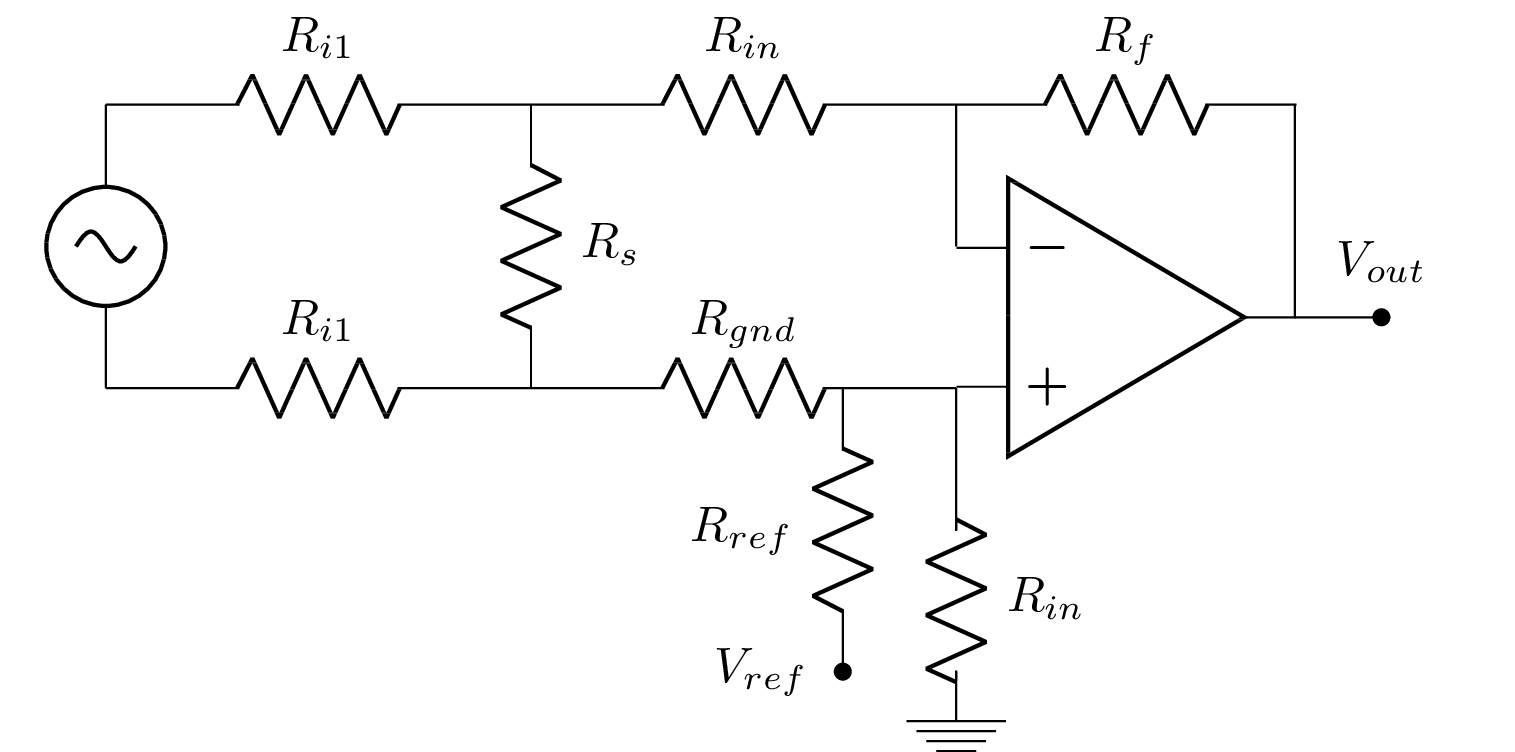
\includegraphics[width=0.8\linewidth]{tikz/voltageCircuit}
	\caption[Voltage sensing circuit]{Voltage sensing circuit}
	\label{fig:voltageCircuit}
	\vspace*{-3ex}
\end{figure}

Although zero crossover detection can be performed in the software, we have provided an analog circuit as shown in figure \ref{fig:triggerCircuit} to perform this task. The zero value for the biased voltage signal could change from circuit to circuit. To adjust to this difference in the voltage level, the crossover reference voltage is generated through a PWM signal generated by the microcontroller. We have observed that the hardware-based zero crossover detection circuit could be useful in increasing the accuracy of voltage and frequency measurement. Zero crossover detection is also useful for accurate measurement of the supply frequency.

\begin{figure} 
	\centering
	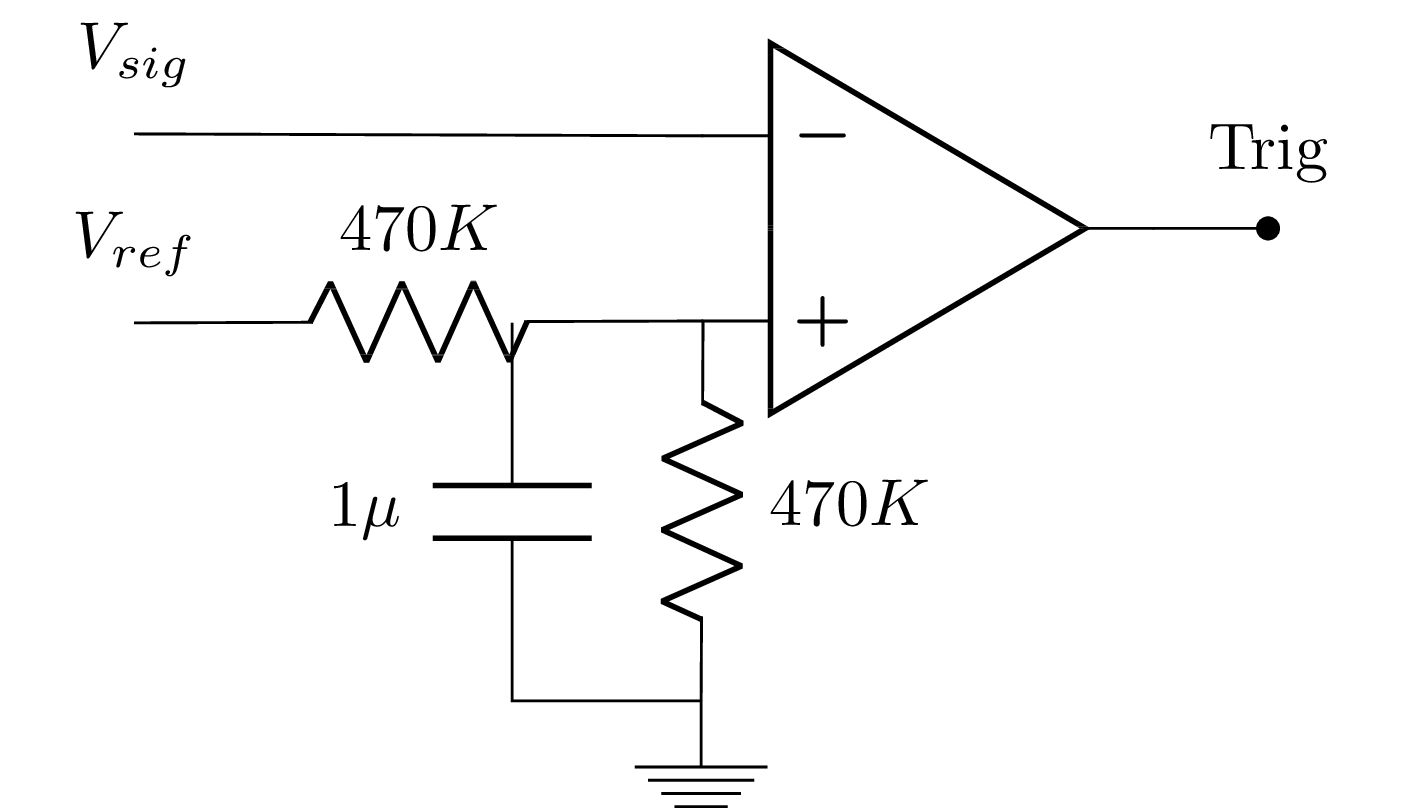
\includegraphics[width=0.55\linewidth]{tikz/triggerCircuit}
	\caption[Zero crossover detection circuit]{Zero crossover detection circuit}
	\label{fig:triggerCircuit}
	\vspace*{-3ex}
\end{figure}

As a micro-controllers can only perform ADC for the voltage, the current signal should be converted to the equivalent voltage signal to make the measurement. Following are the common current measurement methods available

\begin{description}
\item [Series resistance:] Voltage across a precision series resistance is measured to sense the current flowing through it. It is a very popular current measuring technique but it is an intrusive measurement technique which does not provide the isolation of the circuit.

\item [Hall effect sensors:] These sensors are smallest in size, they use the electric field generated by the flowing current through the sensor. This requires the current to be passed through the sensor which is done by cutting the wire and connecting the sensor in series with the load. We have avoided the Hall effect sensor for ease of installation.

\item [Sensor modules:] There are some sensors modules like WL1500 available in the market which provide the voltage output after adding the bias.  %These sensor modules make the circuit smaller but reduce the flexibility of measurement range, therefore, separate modules are required when changing the range of measurement of the smart meter.
These sensors are slightly costlier compared to the other sensors, we are not using this kind of sensor to reduce the cost of the meter.

\item [Current transformers:] Current transformers are the most commonly used current sensing method. they need additional circuits for adding the bias to the sensed signal. They are very accurate, and low in cost which makes them most suitable for the smart meters. The advantages of these current transformers are that by changing a single component (burden resistor) or by just changing the turn ratio of the transformer, the sensitivity of the measurement can be changed.  In our design, we are using the current transformer and a bias adding circuit using a few components as shown in figure \ref{fig:currentCircuit}. This reduces the cost while providing the flexibility of measuring range.

\end{description}


\begin{figure} 
	\centering
	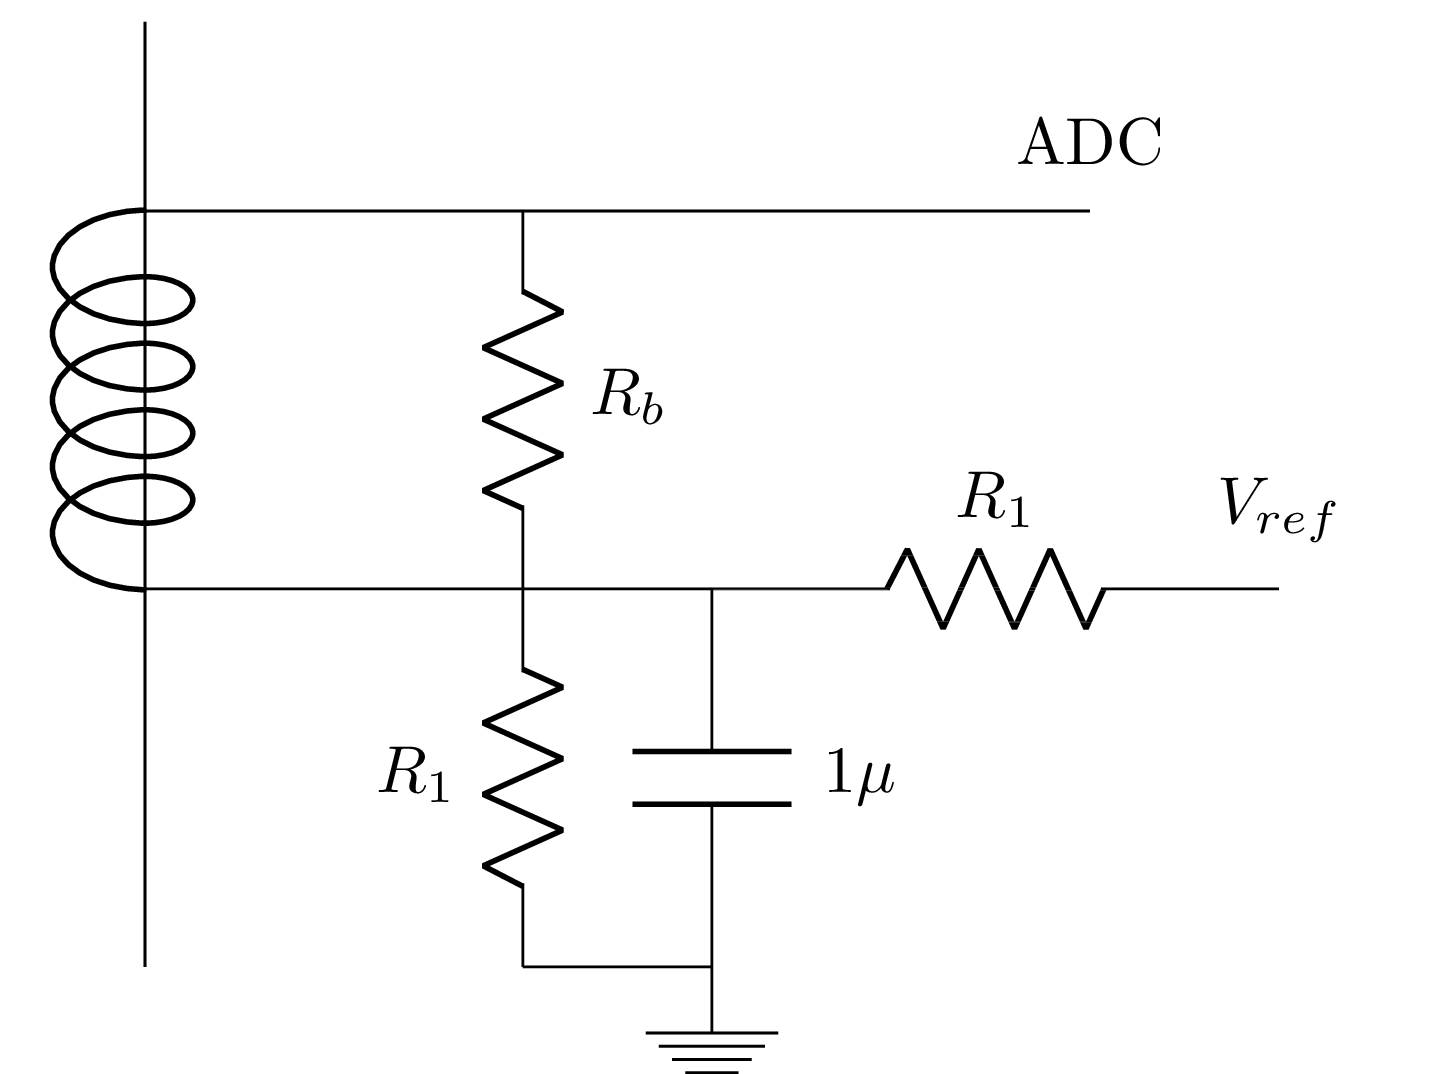
\includegraphics[width=0.5\linewidth]{tikz/currentCircuit}
	\caption[Current sensing circuit]{Current sensing circuit}
	\label{fig:currentCircuit}
	\vspace*{-3ex}
\end{figure}

\begin{algorithm}
	\caption{High level flow of AVR program}
	\label{algo:AVRalgo}
\begin{algorithmic}[1]
\State start timer timeSinceLastAdcComplete
\While{True}
    \If{timeSinceLastAdcComplete $>$ 80}
	    \If{AdcComplete}
		    \State $Q_{adc}.push(v_{adc}, i_{adc})$
		    \State timeSinceLastAdcComplete = 0
		\Else
		    \State Continue
	    \EndIf
    \EndIf
	\If{$! Q_{adc}.isEmpty$}
		\State $v, i \gets Q_{adc}.pop()$
		\State $Q_{avg}.push( v*v, i*i , v*i)$
		\State Continue
	\EndIf
	\If{$! Q_{avg}.isEmpty$}
		\State samples ++
		\State $vv, ii, p \gets Q_{avg}.pop() $
		\State $vv_{sum} \gets vv_{sum} + vv, ii_{sum} \gets ii_{sum} + ii$
		\State $Q_{rms}.push(sqer(vv_{sum} /samples), sqer(ii_{sum} /samples) , v*i)$
		\State Continue
	\EndIf
	\State ...

\EndWhile

\end{algorithmic}

\end{algorithm}

\begin{figure} 
	\centering
	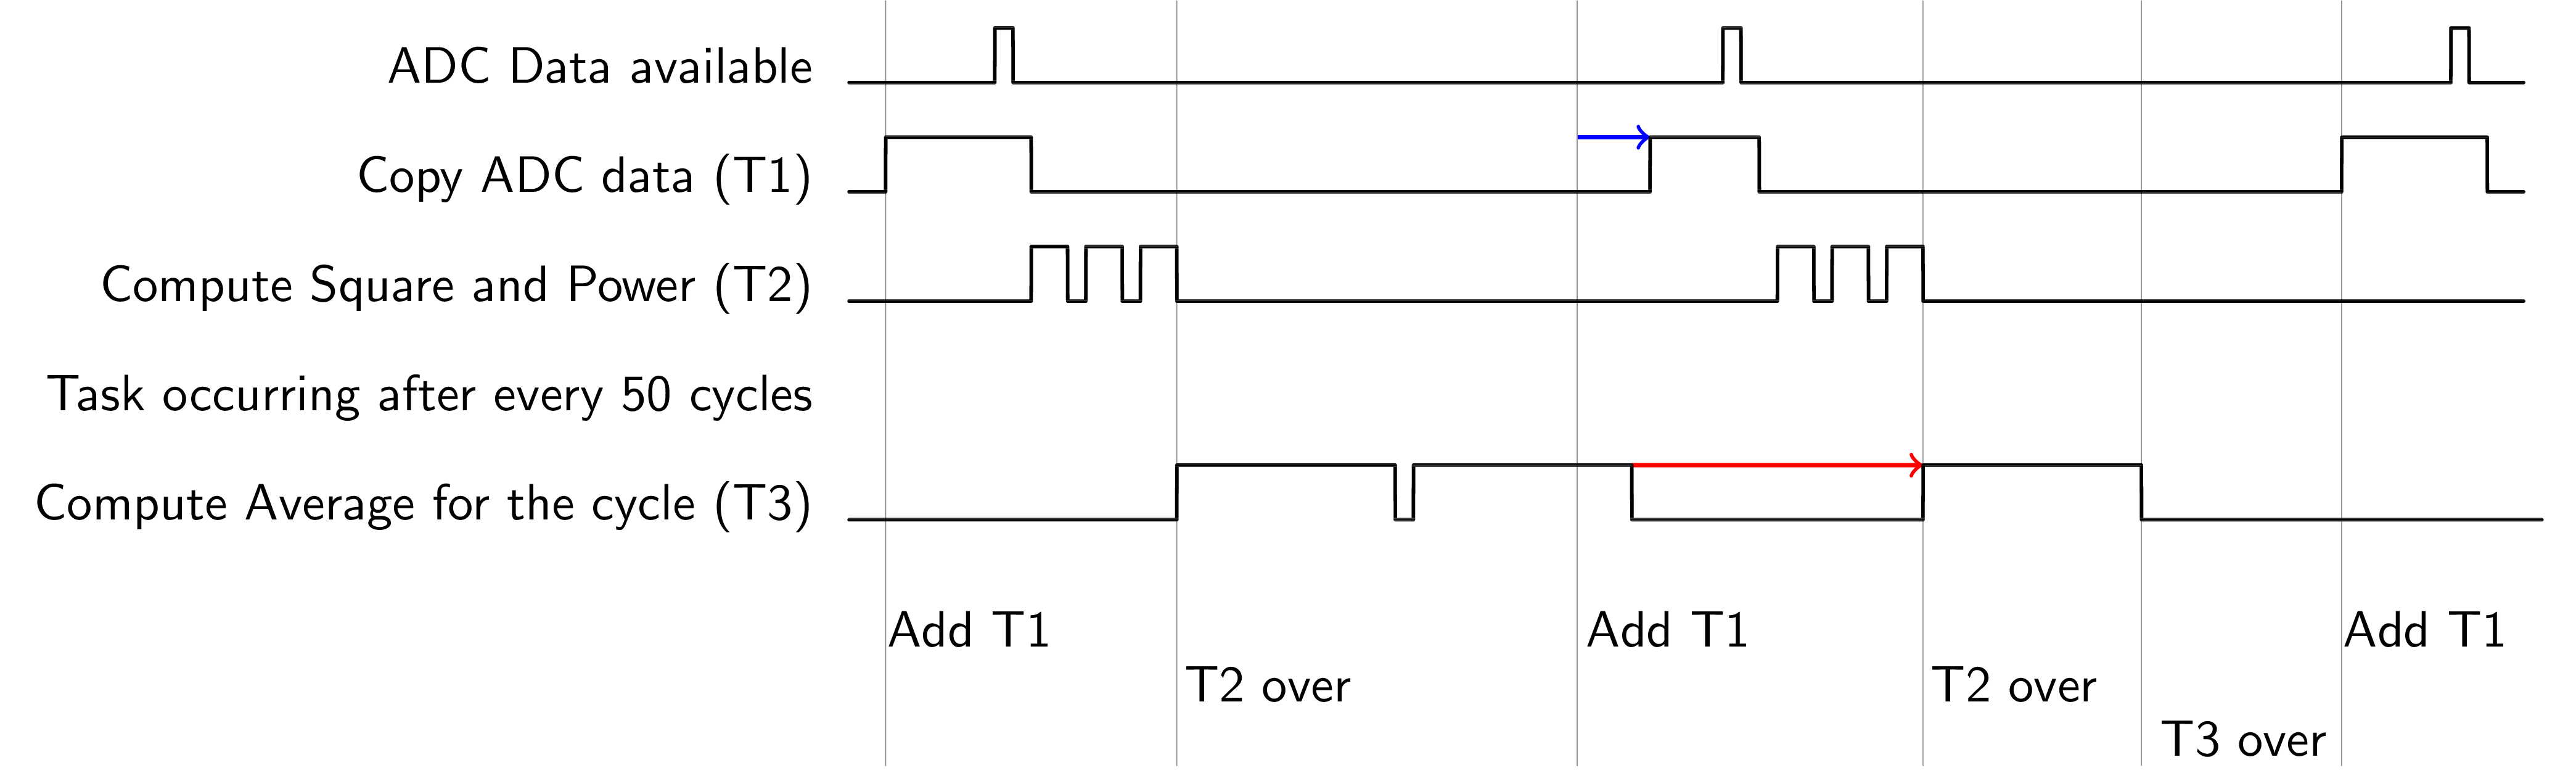
\includegraphics[width=1\linewidth]{tikz/timing}
	\caption[Time utilized by different tasks]{Time utilized by different tasks}
	\label{fig:timing}
	\vspace*{-3ex}
\end{figure}

A meter should perform the operation of sampling, computing the various power parameters like current, power, and power factor, and analyzing the data. These operations are complex and it is difficult to perform these operations together with the energy disaggregation in a single microcontroller. The option adopted by many chip manufacturers is to have multiple microcontrollers on a single chip and perform limited tasks on each microcontroller. These single-chip solutions perform sensing tasks on one microcontroller and computation task on the other and directly provide the average voltage, current, and power consumption as output. Such chips are good for making the smart meters but are not good for disaggregation task as the underlying hardware does not provide the flexibility. Making the slightest change like changing the data refresh rate is also not possible on such hardware.

Hardware like Raspberry-Pi have sufficient processing power to perform sensing and processing tasks but it does not have an onboard ADC. Such single-board devices are good in computation but bad in real-time analog sensing capabilities.



% add following table
%Operation  uint8          int16          int32          int64          float**
%+                  63^             884           1763           8428          10943
%*                  125^            1449          4592          57038        10422
%/                 15859^^      15969       41866*       274809      31951
%sqrt                                54251       54448        70884        47127
%micros()                                            3524

The time required by an AVR microcontroller, running at 16 MHz, for different operations is given below.

\begin{equation}
V_{rms} = \sqrt{\frac{\sum_{i=0}^{n} ((k* (S_i - S_{cross}))^2}{n}}
\end{equation}

For computation of $V_{rms}$ will be $ n * \tau_{ia} + n * \tau_{fm} + n * \tau_{fm} + n *  \tau_{fa} +  \tau_{fd} +  \tau_{fs}$ where the first term is subtracting $S_{cross}$, second term is for multiplication with the constant $k$, third term is for computation of the square, forth is for the summing all the squares. The term  $\tau_{fd}$ is for the division by $n$ and  $\tau_{fs}$ is for performing the square root.

For 96 samples per cycle, the time required for computation based on table \ref{tab:ComputationTime} will be $~ 4.4 ms$ for just voltage calculation. After including the time required for computation of current and power, there will not be enough time left for any other task. Same computation can be performed much lesser time instead if the following computation is done

\begin{equation}
V_{rms} = k * \sqrt{\frac{\sum_{i=0}^{n}(S_i - S_{cross})^2}{n}}
\end{equation}

same result is obtained in only $ n * \tau_{ia} + n *  \tau_{im} + n *  \tau_{ia} +  \tau_{id} +  \tau_{is} +  \tau_{fm}$ us or $~ 1 ms$.  The overall execution time and the frequency of execution of different tasks is given the table \ref{tab:taskTimeRequirement}


\begin{table}[htb]
	\centering
	\caption{Time required to perform mathematical operations}
	\begin{tabular}{@{}llr@{}}
		Symbol & Description & Time in $\mu s$ \\
	\midrule
		$\tau_{ia}$  &  int32 addition  & 2 \\
		$\tau_{im}$  &  int32 multiplication  & 5 \\
		$\tau_{id}$  &  int32 Division  & 42 \\
		$\tau_{is}$  &  int32 Sqrt  & 55 \\
		$\tau_{fa}$  &  float addition  & 11 \\
		$\tau_{fm}$  &  float multiplication  & 16 \\
		$\tau_{fd}$  &  float Division  & 32 \\
		$\tau_{fs}$  &  float Sqrt  & 48 \\
	\bottomrule
	\end{tabular}
	\label{tab:ComputationTime}
\end{table}

\begin{table}[htb]
	\centering
	\caption{Total time required for each task}
	\begin{tabular}{@{}llrrrr@{}}
		 Task  &  Deadline  &  Deadline  &  Processing  &  Execution  &  Total \\
		  &  type  &  time $\mu s$ &  Time $\mu s$ &  count  &  time $\mu s$ \\
	\midrule
		Copy data from ADC buffer  &  Hard              & 100 & 2 & 10000 & 20000 \\
		Compute power                &  Soft              & 100 & 5 & 10000 & 50000 \\
		Compute  square of each sample              &  Soft              & 100 & 5 & 10000 & 50000 \\
		Compute average for a cycle  &  Soft              & 2000 & 30 & 50 & 1500 \\
		Compute square root for RMS  &  Soft              & 2000 & 130 & 50 & 6500 \\
		Compute   average across cycles       &  Soft              & 2000 & 130 & 50 & 6500 \\
		Final   data preparation  &  Soft              & 2000 & 100 & 50 & 5000 \\
		Total  &   &   &   & 30200 & 139500 \\
	\bottomrule
	\end{tabular}
	\label{tab:taskTimeRequirement}
\end{table}

The sensing section is responsible for collecting the desired data and perform appropriate action based on the detected events. We have put minimum possible functionality in this section. Our approach is to remove any processor intensive functionality from this section which can be performed outside this section. Its tasks are as follows

\begin{itemize}

\item To measure voltage and current
\item To compute the instantaneous power
\item To identify the start and end of the cycle
\item To compute average and then RMS values for voltage and current
\item To compute the power consumed during a cycle
\item To compute the power factor
\item To generate signals when the data is available
\item To send data

\end{itemize}


The sensing module can act as an SPI slave or UART host to communicate. It also generates a hardware signal when the data is available for reading.


There could be multiple approaches to executing all the tasks timely. We compared multiple such approaches and evaluated the advantages and disadvantages of these approaches. The sensing section can be implemented in a large number of microcontrollers which support ADC and SPI interface like AVR, PIC, ARM, etc. We have done our sample implementation in a lower end processor Atmega32p \cite{ATmega328P8bitAVR}. We have used the Arduino Pro Mini because of its small size and ease of availability. This processor runs at a clock speed of 16 MHz and does not provide the DMA control of the ADC hardware. This processor provides a single 10 bit ADC converter with a maximum of 12KHz sampling frequency which is sufficient for this purpose. %In such low profile microcontrollers, it is difficult to implement the task compared to the ARM processors like STM32 series which runs at least 48 MHz frequency and provide DMA access of the 12 bit ADC of a much higher sampling rate.

The sample implementation is done on a lower end microcontroller because it can be easily migrated to any microcontroller with more power. It provides a benchmark for the functionalities that can be supported by the sensor section on which additional functionality can be built. It also provides a low-cost implementation for building a standard smart meter.

As the processor does not provide DMA to read the ADC data, ADC data should be read before the next ADC is generated. This provides limited time for performing computationally complex tasks. If any task takes twice the time as that of the interval between two ADC conversion, the ADC sample will be lost. The processor also provides only one ADC hardware therefore both the voltage and the current should be sensed by different channels connected to the same ADC hardware. In such hardware, it is impossible to sense the two channels simultaneously, therefore one channel (current) is sensed and the value for the other channel (voltage) is interpolated by taking two voltage readings and interpolating them.

A large number of Real-time operating systems (RTOS) are available to manage multiple tasks. Embedded processors do not have huge processing powers, therefore, the minimum time-slice for scheduling a task is generally very high. If this time slice is reduced beyond a certain limit, a majority of the processors time will be spent on context switching and not enough time will be left for processing. Therefore the time-slice provided by the RTOS is not sufficient to make a thread for analog sensing.

Table \ref{tab:taskTimeRequirement} shows the total time required to execute different tasks in the AVR processor running at a 16 MHz. At the clock frequency of 16 MHz, the ADC clock frequency can be set at a maximum of 25 KHz. As each conversion in AVR takes 13 ADC clocks, the ADC sampling rate is 125 KHz /13 = 9615 Hz at this frequency.

In the AVR microcontrollers, the ADC conversion is not buffered, this makes it compulsory to read the conversion registers before the completion of the next conversion. The copy data operation from the ADC buffer is a hard deadline task, failing which will make the overwrite of the buffer and therefore loss of the sensed value thereby making the final value of the meter, less accurate. The reading of ADC is done in an interrupt handler which needs around 2-3 $\mu s$ to process. This is the best that can be achieved on this processor. The processor hardware does not support ADC scan mode, therefore channel is changed in software. Since ADC is in the auto mode and starts immediately after finishing the previous conversion, channel change should be done before the next ADC starts. To make sure that this deadline is never missed, this task is also done in the ADC conversion complete interrupt.

As the number of context switches is too high, implementing tasks in the preemptive RTOS, which requires high context switching time, will make the system infeasible. Because of this reason the tasks are implemented as the collaborative scheduler as stated in the algorithm \ref{alg:algo1}. As the non-preemptive scheduler, it is highly dependent on each task to follow the following rules

\begin{enumerate}
\item Tasks give the control back to the scheduler within maximum permitted time.
\item  While returning the control back to the scheduler each task informs the scheduler about its status in the returned value. The possible return status should be one of the following.

\begin{description}

\item [Continue:] This return status indicates that the task has pending work but it is returning control to the scheduler because it has finished a processing unit.
\item [Finished:] This return status indicates that the task has no pending work.
\item [Blocked:] This return status indicates that the task has pending work but it could not complete it because of resource unavailability.
\end{description}
\end{enumerate}

Figure \ref{fig:timing} display all the task and their relative execution cycle, a task that requires a long time are divided into small subtasks that return control to the scheduler when a subtask is finished.

The system clock in maintained by a separate timer and is used by the scheduler to identify if a task can be called. A process will be called if the following conditions are met
\begin{itemize}
\item The task is not blocked for resources
\item The time requirement of the processing unit of the task will not violate the deadline for next occurrence of any of the hard deadline task.
\end{itemize}

All the tasks are pipe-lined where the data processed by one task is consumed by the next task. The data buffer between the processes is implemented as queues but the restricted amount of memory available on the processor enforces the queues to be very small. The time required for each task is dependent on the number of elements present in the queue. Therefore when any process is delayed its priority will increase because the queue is less empty and the processing requirement increase as the queue is more filled.

\begin{table}[htb]
	\centering
	\caption{Comparison of features}
	\begin{tabular}{@{}lcr@{}}
		Feature & Current Smart Meter & Our Samat Meter \\
	\midrule
		Voltage & Yes & Yes \\
		Current & Yes & Yes \\
		Power & Yes & Yes \\
		Frequency & Yes & Yes \\
		Reactive Power & Yes & Yes \\
		Power Factor & Yes & Yes \\
		Active suseptence & No & Yes \\
		Reactive suseptence & No & Yes \\
		Power Signature & 1 Hz (continious) & 50 Hz (event based) \\
		High frequence voltage & No & 9.6 KHz (event based) \\
		High frequence current & No & 9.6 KHz (event based) \\
		High frequence power & No & 9.6 KHz (event based) \\
		Reading method & Pull & Push \\
		Protocol & Modbus & Multiple \\
	\bottomrule
	\end{tabular}
	\label{tab:meterFeatures}
\end{table}

A smart Meter capable of load disaggregation should be tested with a large number of appliances. It is not practical to use actual load to design such meter because it is expensive in terms of time, cost and space. As high voltage is involved, a lot of precautions should be taken while conduction such tests. To speed up this task we developed a voltage and current signal simulator. This simulator enables us to work with low voltage circuits only and test out a large number of appliance combinations without running the actual appliance. This simulator can replay the appliance behavior by using high-speed DAC (digital to analog converter).  As the power measurement requires both voltage and current sensing, two ADC are used to generate these signals.

We have used the NUCLEO-F303RE \cite{NUCLEOF303RESTM32Nucleo64} development board to make this simulator.
The microcontroller on this board has DMA to transfer data from the waveform buffer to the 2 DAC to create smooth analog signals. DMA is used to feed data in both the DAC channels simultaneously. In order to use second the DAC on the nucleus board, the 0-ohm resistor connected to the pin 13 led should be removed, thereby disabling the led.

By taking only a few data samples from an actual appliance or using open data samples like PLAID \cite{gaoPLAIDPublicDataset2014}, we can simulate a large number of appliances in a variety of modes without even procuring the actual appliances. The simulator can also generate different frequency and voltage level data from a single sample collected from the actual appliance.


	\chapter{Detecting System Problems}
\subsection{Detecting Spikes}
\begin{figure} 
	\centering
	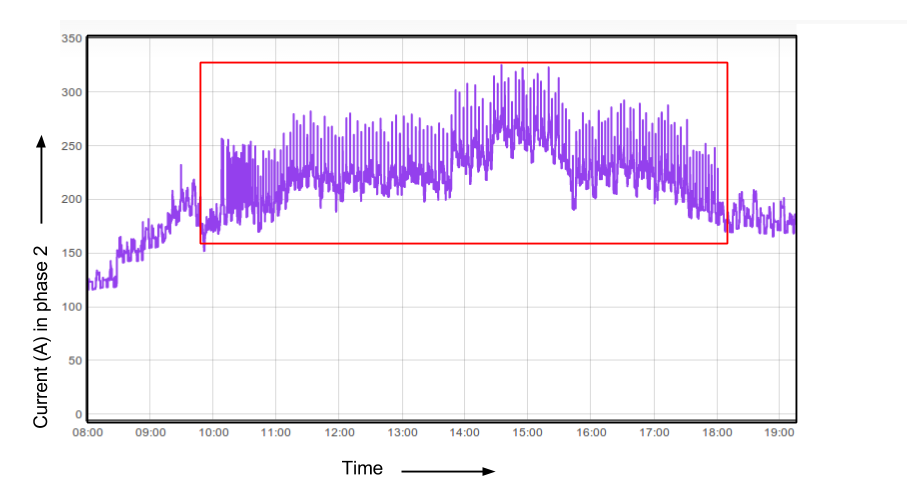
\includegraphics[width=1\linewidth]{images/spike4_new}
	\caption[Spikes]{Spikes}
	\label{fig:spike4}
	\vspace*{-3ex}
\end{figure}

%\begin{figure}
%\centering
%\includegraphics[width=1\linewidth]{images/G3_M1_20140107_12}
%\caption{Current spike are generated when an appliance is switched on}
%\label{fig:G3_M1_20140107_12}
%\end{figure}

Spikes are very regular phenomenon on a power system, they occur whenever an inductive  appliance is switched on, Figure \ref{fig:G3_M1_20140107_12} shows such a spike caused by starting an AC. These spikes are generated because of high starting torque required by the induction motors. Normally this startup current could be up to 2-3 times the normal running current of the appliance. Motor consume a constant current once it is started and running.  

When such appliance fail to start, the starting high current is drawn but the constant current after the initial startup phase is not drawn. This failure to start can be observed as a current or power spike as shown in the figure \ref{fig:regularSpike}. 

Detecting such spikes is a challenging task because of following reasons 
\begin{itemize}
	\item Too many spikes: Spikes are very common in the a electrical system therefore it is difficult to find the spike caused by faulty appliance.
	\item Too many appliance: Large number of appliance are connected to the system which makes the isolation of the faulty system vary difficult.
\end{itemize}




%Spikes which are associated with appliance switching should not be considered as a fault. Power consumption in the system is generally steady with transients for starting or stopping the appliance. When we pass the data from a median filter, spikes get removed from the data without impacting the load pattern of the data as shown in the figure. used to identify Spikes without appliance switching as follows. 

Spikes are a very regular phenomenon in a power system. Whenever an appliance with a capacitive load is switched on it draws a very high current. Many appliances with moving parts also require high power to put the moving part in motion. The appliance draws steady power once the desired speed is achieved. In normal operation, the spike is almost always followed by an increase in the load. 

Many heavy load appliances such come with a protection mechanism that switches off the appliance when desired parameters are not achieved. An air conditioner may switch off if the compressor motor is not rotating with the desired speed or the coolant pressure is not correct. When such failure occurs, the spike is not followed by an increase in power. An appliance like ACs also switches on the compressor when a higher temperature is detected. This switching ON and OFF operation is repeated indefinitely which results in spike at a regular interval for a long duration. 

Such faulty ACs may impact the health of the system and other ACs adversely. When many air conditioners are installed in building these faulty airconditioners go undetected for a long time. It is not easy to detect such spikes when a large number of appliances are installed in a building which causes regular spikes. To detect the presence of such a faulty appliance in a building we use the 1 Hz power consumption data collected at the mains meter. Let vector $\vec{p}$ is the time series of the power consumption samples collected periodically between time $0$ and  $n$. 

%$$\vec{p} = \left \{  p(t) : t = 0 ... t_{max}    \right \}$$
$$\vec{p} = [ p_0, p_1, p_3 ... p_n  ]^T $$

We apply the median filter to this data to remove the spike from the data. As the power consumption is generally steady, median filter $medfit_m$ to obtain a spike free power consumption data. The width of the median filter is $2 m + 1$ where $m$ is the number of sample for which the spikes are observed. 

$$ \vec{q} = medfit_m(\vec{p}) $$

The difference between $\vec{p}$ and $\vec{q}$ provides data that contains only the spikes. These are all the spikes observed in the mains meter and could be because of faulty as well as non-faulty appliances. In the second step, we identify the change in a load before and after the spike (delta) $\vec{q}$. If the difference between the two power is not significant than these spikes could be caused by the faulty appliance. 

$$T_+ = \left \{ t :  p_t >  p_{t-1} + p_{threshold}   \right \}$$

$$T_a = \left \{ t :  q_t >  q_{t-1} + q_{threshold}  \right \}$$

$T_a$ are the time instances when some appliance is switched on and $T_+$ are the time instances when a positive transition is observed in $\vec{p}$. $p_{threshold}$ and $q_{threshold}$ can be chosen to based type of the appliances and magnitude of spike generated by these appliances. If a time instance is present in $T_+$ and not present in $T_a$ it is a spike probably not associated with appliance switching.

$$ T_s = \left \{ t :  t \in T_+,  t \notin T_a \right \} $$  

Based on the values of $p_{threshold}$ and $q_{threshold}$ we may get excess number of spikes or fewer number of spike. In our observation. A spike that is not followed by a change in load is not a confirmation of a faulty appliance. Such a situation can be observed if multiple appliances operate simultaneously or the steady-state power drawn by the appliance is less than the threshold selected.

To identify the faulty AC from these large numbers of false positive spikes, the cyclic nature of the spike should be identified. The time interval between the consecutive spikes are identified by plotting histogram of the time interval between spikes. An unusual high value is observed in the plot for a time period equal to the periodicity of the faulty appliance. Our objective is to identify the appliance that caused the spikes at these time instance. This can be used to identify the time instance when the spike is observed. The meter installed at the building level is sufficient to identify the presence of spike in the data. 

\begin{figure}
	\centering
	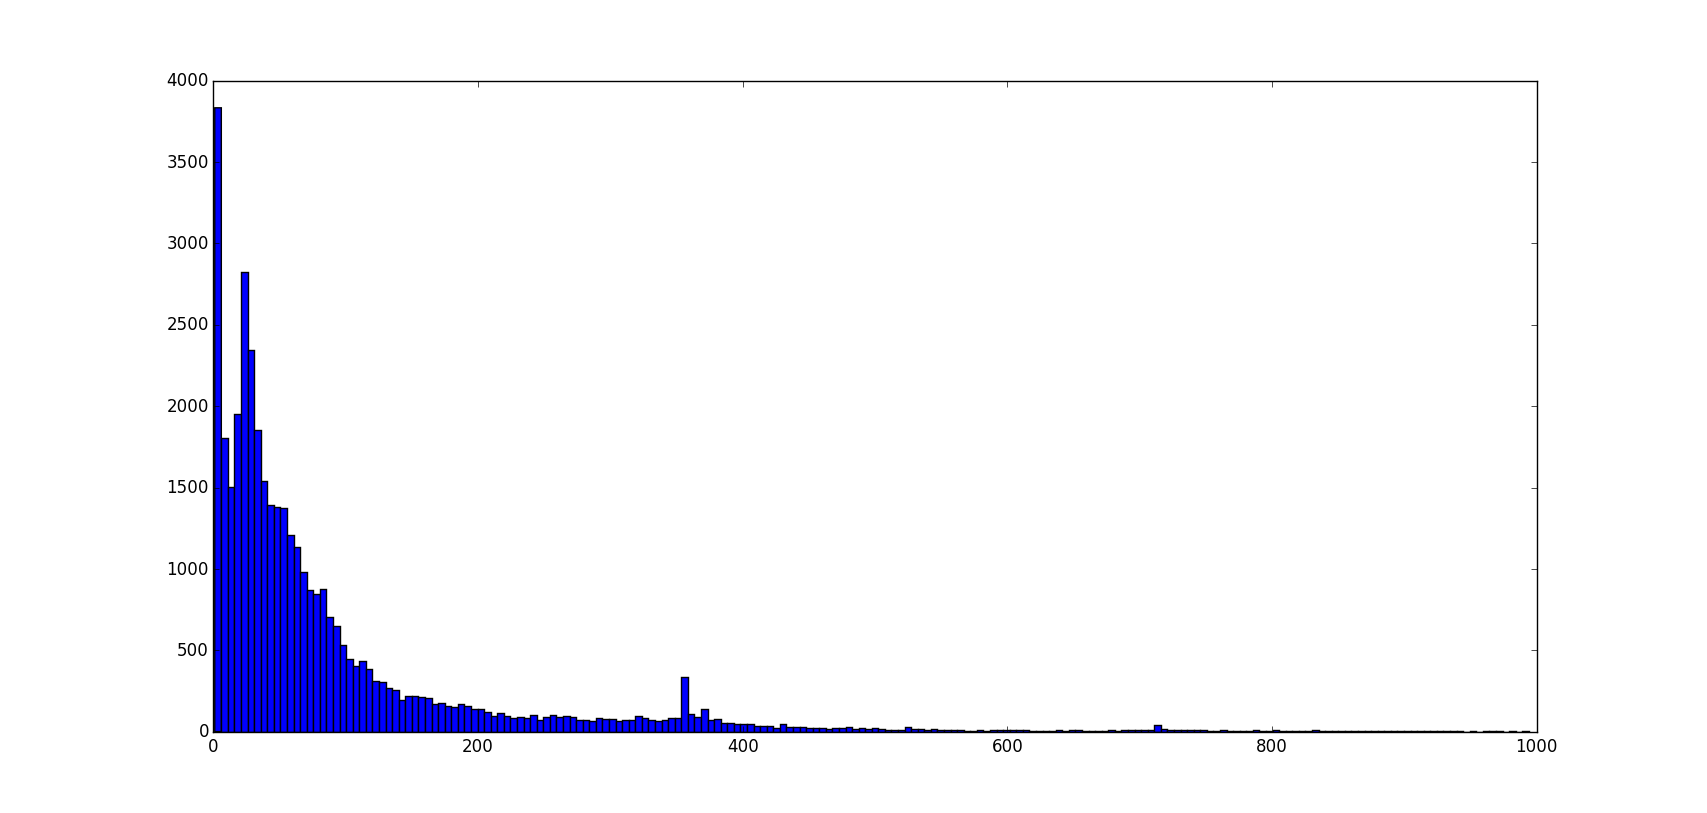
\includegraphics[width=0.7\linewidth]{images/freq_histogram}
	\caption[Spike Histogram]{Spike Histogram}
	\label{fig:freq_histogram}
\end{figure}

An induction motor is used to compress the coolant in the AC. Amount of work required to compress the coolant increases with the quantity of already compressed coolant. If motor is started when the coolant is already compressed, torque required is too high which causes even higher starting current that can damage the motor. To avoid the risk of damage, Air Conditioners are prevented from starting when the coolant is compressed. Simple technique to do this it to allow the coolant to decompress before starting the motor. It is assumed that when the motor stops, coolant is maximum compressed and time required to decompress the coolant to a favorable level is computed, which can be termed as conditioning delay. Once the motor is stopped, it is allowed to start after only after conditioning delay. In case of failure, timer is initiated and the Air Conditioner attempts to start again after conditioning delay. In a faulty Air Conditioner this cycle is repeated continuously and is observed as repeated spike of power or current.

To find periodic spike, time interval between the consecutive spikes are computed and a histogram of the time interval is plotted. The frequency of time interval follows an inverse square curve as the spike occurrence rate is suppose to be a normal distribution. On this curve a peak is visible which indicates an unusually high rate of spike recurrence after 355 second. The high frequency value is for a time period equal to the periodicity of the faulty appliance. Presence of this peak indicates that there is faulty appliance in the system. Once the presence of faulty appliance is confirmed, next objective is to identify the location of this faulty appliance.


\subsection{System layout Correction}
When smart meters are installed for energy measurement, some of the minor aspects of the installation are ignored. One such aspect is the connection polarity of the three phases. For some meters in our setup, the polarity was not the same as the mains meter. This difference in phase connection does not cause any issue while measuring energy consumption but turns out to be critical for comparing phase voltage, since comparing the voltage of two different phases will give wrong estimates. We understand that this is a common problem and will be more prevalent when single phase meters are installed. The variation in the voltage sensed at such a meter can be used to identify the correct phase connection for the meter.

When we install solar roof-tops both in residences and in larger buildings, we need to ensure that  a panel is connected to the right phase. In fact, most building managers have an incorrect circuit map of the building which can be quite large \& complex in commercial buildings. So identifying phase at every point and socket correctly is an important aspect of correcting the circuit map of a large building. Since buildings are also commercially billed, they are penalized for imbalanced phases by the utility that one cannot address without identifying the phase of different loads in the building.

When the voltage is observed it varies in a narrow range, and all the three phases appear to change in harmony when observed for a long time interval, but for a very short duration, the variation is distinct for each phase. This can be observed in the figure \ref{fig:voltageChanges} where the voltage for the three phases sensed by the mains meter changes differently. This difference in variation can be used to identify the correct phase of the meter for which the phase is not known.
%rg
%Voltage sample for one minute (60 samples) are take from the meter with the unknown phase $(v_x)$ and the reference meter $(v_1, v_2, v_3)$ are taken.
%The correlation coefficient for all the combination of voltages for the reference meter are computed. If all the correlation coefficients are lower than a threshold, correlation coefficient of the voltages of the reference meter with the unknown meter are measured. If the correlation coefficient for the reference meter are not lower than the threshold the process is repeated for the next one minute interval.
%A one minute sample of voltage, from each phase of the mains meter, is used as a reference for this purpose. The voltage series for each phase is collected given by $v_1$,  $v_2$, and $v_3$.  Correlation coefficients are computed for all the voltage pairs. If all the correlation coefficients are lower than a threshold, a voltage sample for the same duration for the unknown meter is taken, and its correlation coefficients with the three voltages are computed.
%The meter is assigned the phase for which the  correlation coefficient is highest. In the figure \ref{fig:Freq_change}, the voltage observed at meter \textit{with Unknown phase} is also shown. The correlation coefficient of this meter is highest with $v_1$ as shown in the table \ref{tab:corr_coef} which means that this meter is connected with phase 1.

We take the time series sample of the voltage at the reference meter and make sure that there is sufficient difference in the pattern for the three phases. This is made sure by computing the correlation coefficients for three phases. Should any of the correlation coefficients be more than a threshold value, the sample is discarded and the next sample is taken. We utilized samples of 6-minute duration and the threshold of 0.85 for this purpose. Approximately 40\% of the samples are discarded because of this criterion. In such a case, the sample starting time is increased by 30 seconds and the process repeated with the new sample.

The voltage sample at the same time is used to compute its correlation coefficients with the three phases of the reference meter. If the highest correlation coefficient is higher than another threshold (0.95), its phase is assigned to the unknown phase else the process is started from the beginning. The worst accuracy obtained by this method is 99.83\%. Because of the discarding of the samples, the time required to identify the phase varies. In 88\% of the cases, the phase was identified in one attempt. In our scenario, during the night time when there is less variation in the voltage, the algorithm has lower chances of identifying the phase voltage in one attempt.
%rg end
Phase correction is a one time task that is performed for all the meters once and the results obtained are saved in a mapping table which is used for translating the phase name while using the meter data.

\begin{figure} 
	\centering
	\includegraphics[width=1\linewidth]{images/voltageChanges}
	\caption[Variation of unknown phase and al the 3 known phases during a minute]{Variation of unknown phase and al the 3 known phases during a minute}
	\label{fig:voltageChanges}
	\vspace*{-3ex}
\end{figure}

\begin{figure} 
	\centering
	\includegraphics[width=1\linewidth]{images/voltageforday}
	\caption[Variation of supply voltage during a day]{Variation of supply voltage during a day}
	\label{fig:voltageforday}
	\vspace*{-3ex}
\end{figure}

\section{Smart Meters}
A good number of energy meters are designed by researchers to serve different objectives, like plug monitoring, ease of installation, energy harvesting or controlling the attached appliances but none have focused on providing all the data required for the objective of energy disaggregation.

PowerBlade \cite{debruinPowerBladeLowProfileTruePower2015} defined and performed the tasks of reducing the AC mains voltage and current for the purpose of measuring, calculating power and communicating the same. Our meter extends tasks of the smart meter by communicating the high-frequency values of current and voltage required by many disaggregation algorithms \cite{hassanEmpiricalInvestigationVI2014} \cite{guptaElectriSenseSinglepointSensing2010} \cite{gulatiDepthStudyUsing2014} \cite{BOLT} and communicating only when a significant change in the values is observed.

Kill A Watt \cite{KillWattMeter}, and many similar plug level meters are available in the market. These meters are only suitable to identify the power consumption of appliances that can be plugged into the sockets. They are not good for continuous monitoring of the appliance or measuring the power consumption of the appliances that are directly connected through the switchboard.

There are some energy meters like \cite{mogheDesignLowCost2010}, \cite{caiSelfpoweredSmartMeter2012}, \cite{debruinMonjoloEnergyharvestingEnergy2013}, and \cite{villaniContactlessThreephaseAutonomous2016} which focus on the ease of installation and use energy harvesting to run the meter. The limitations of these meters are the nonavailability of energy to harvest when the appliance is off, they have to compromise on accuracy also because of energy constraints. IoT based smart energy metering system \cite{al-aliIoTBasedSmartUtility2018} \cite{yaghmaeeDesignImplementationInternet2018} focuses on sensing other parameters or collecting water or gas consumption data together or collecting temperature humidity, and air quality data. The act as the data collection agents which take the responsibility of sending the collected data to the servers.

Visualization platforms like \cite{luDesignImplementationPower2016} focus on using the existing architecture of the power system for information acquisition and display it to the user to provide better insight into the energy consumption pattern and reducing the power consumption. Our meter will enhance the capabilities of such visualization platforms by enabling them to provide a better understanding of the appliance being used. As our meter can be used without additional communication hardware and require less communication bandwidth, energy visualization platforms can use such services efficiently at a lower cost.

REDD \cite{kolterREDDPublicData2011} is a very popular home energy consumption data set. It provides continuous low-frequency power consumption data and high-frequency current and voltage data when a transition in power consumption is observed. The technique used by REDD is very efficient in reducing the storage requirement for the data set. Out meter also utilizes a similar technique to reduce the storage for sending the power readings from the meter.

Studies have suggested that the biggest obstacle is to identify the cost bearer for the new meters \cite{Romer2012}. A cheaper meter that can be upgraded will help in overcoming such obstacles. Once installed, a smart meter can become a proxy for the water and gas meter \cite{Zivic2015} too. When Smart meters become omnipresent, they will be performing multiple tasks including sensing other environmental parameters and controlling appliances \cite{tripathyPrepaidEnergyMetering2010} \cite{ganuNPlugSmartPlug2012} and identifying faulty appliances \cite{palaniPuttingSmartMeters2014}.



	- System capacity issues: A client-server architecture is not suitable for such massive data collection because it may result in a bottleneck because of the server side delay in writing the data to the disk. We have adopted a multi-tier architecture suitable for a large number of sensor data logging, using an MQTT publish-subscribe router.

\begin{itemize}
 \item Raspberry-pi based data aggregator can collect data from a number of smart meters and store them locally on the SD cards. These SD cards and not suitable for very frequent writing, therefore, local writing should is only performed only when the server is not reachable. Writings should be performed in batch instead of writing every sample to further reduce the wear of the SD cards.
\end{itemize}

\begin{itemize}
 \item Wrong labeling of data: because the meter has only 255 unique IDs and it does not provide the timestamp these two fields should be added to each sensor data sample. Both of the fields are critical for processing the data and any wrong value in these fields can result in the wrong interpretation of the data.
\end{itemize}

Automatic discovery of the sensor was implemented in the Raspberry-pi application, this enabled the Raspberry-pi to automatically configure itself. Each meter holds a meter ID, which is maintained unique in a building.  All the raspberry-Pi holds the same code and the only configuration maintained is the building name. All the details of the meter are stored on a server and can be accessed through a rest API by providing only the meter id, and the location. This made configuration of devices easy and a single spare Raspberry-Pi can be made to replace any problematic raspberry pi without any configuration change. This reduced the human error while configuring the Raspberry-pi or replacing the faulty one less error prone.

\begin{itemize}
 \item Loss of data due to network unavailability: Previously we did not have any mechanism to send the data collected when the server connection was not available.  Even though the data was logged locally it was not sent to the server and got lost.
\end{itemize}

\begin{itemize}
 \item An automatic recovery mechanism was implemented to send the data saved on the SD card during offline status. Offline data is sent to the server through the same MQTT channel to avoid duplicate coding and reconciliation of the data.
\end{itemize}

The auto recovery mechanism in the system allowed us to focus on our research instead of fixing repeating errors as the system can recover from most of the common errors without any manual intervention. Our data collection is now the world-class quality and we are in the state of making the data publicly available.

\section{Correcting Data Collection Errors}
\begin{figure} 
	\centering
	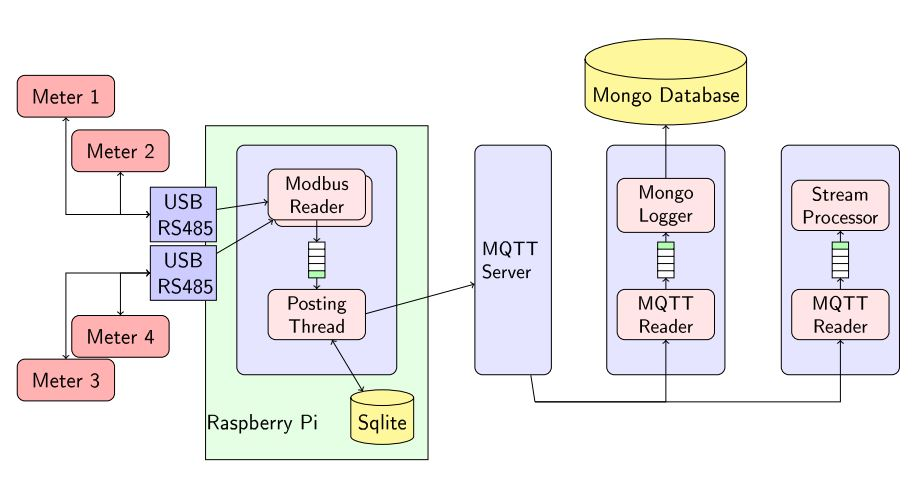
\includegraphics[width=1\linewidth]{images/dataCollection}
	\caption[Component diagram of data collection architecture]{Component diagram of data collection architecture}
	\label{fig:dataCollection}
\end{figure}

\begin{figure} 
	\centering
	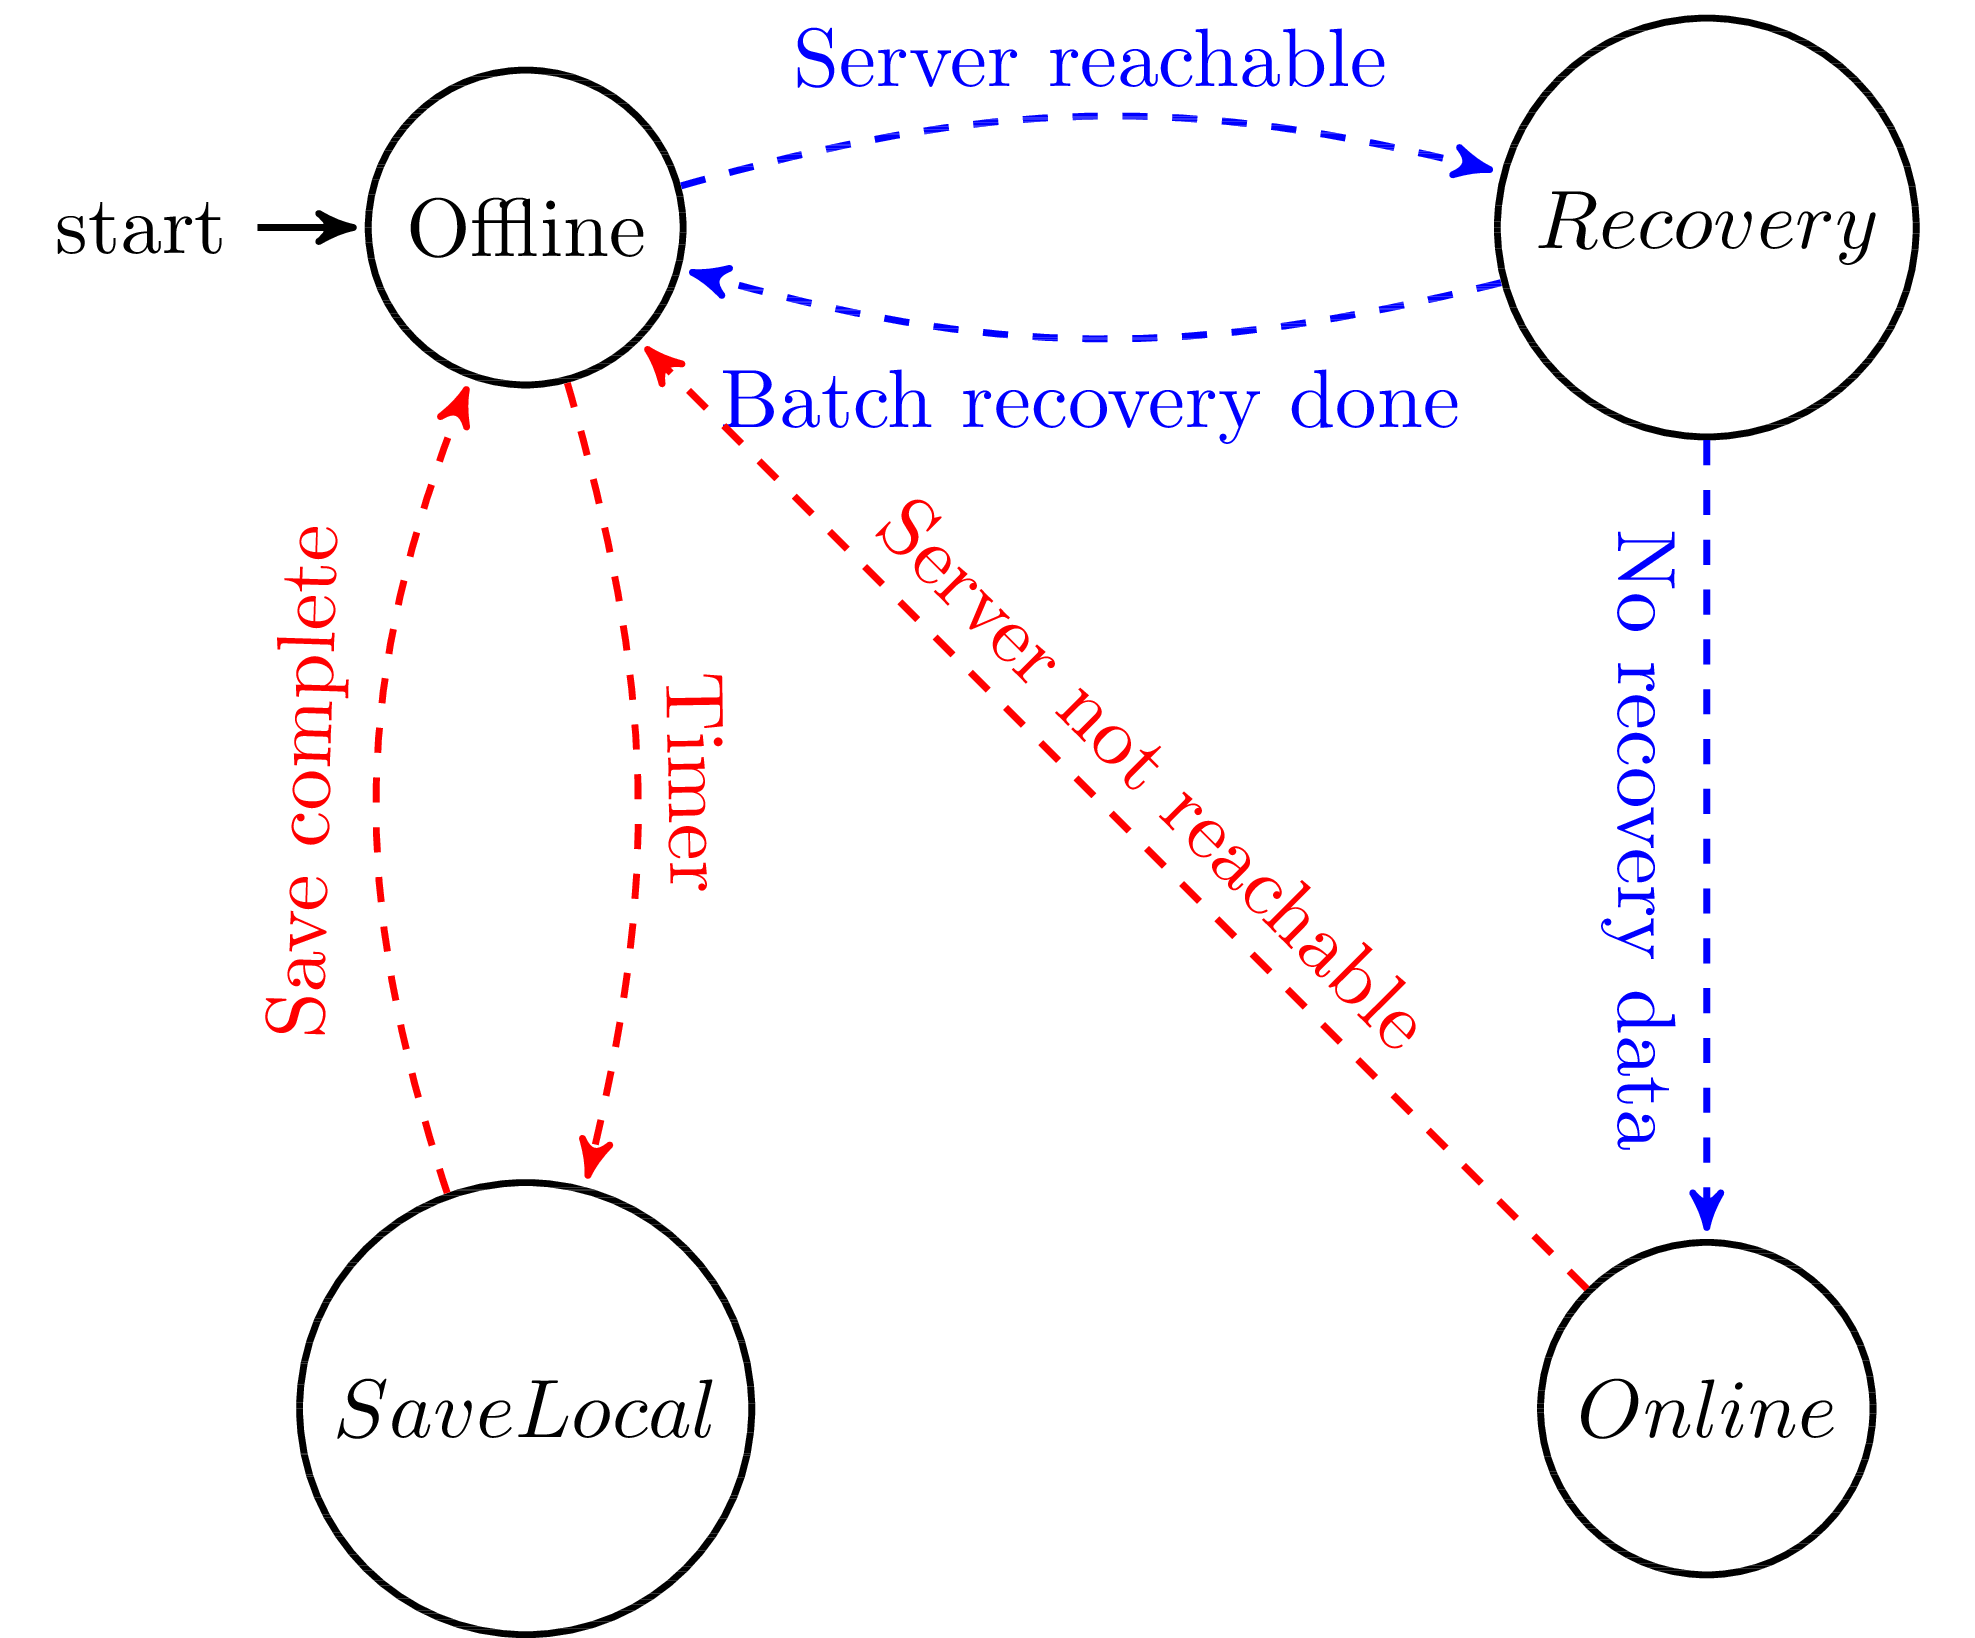
\includegraphics[width=1\linewidth]{tikz/statLogger}
	\caption[State diagram of the data logger]{State diagram of the data logger}
	\label{fig:statLogger}
\end{figure}

\begin{figure} 
	\centering
	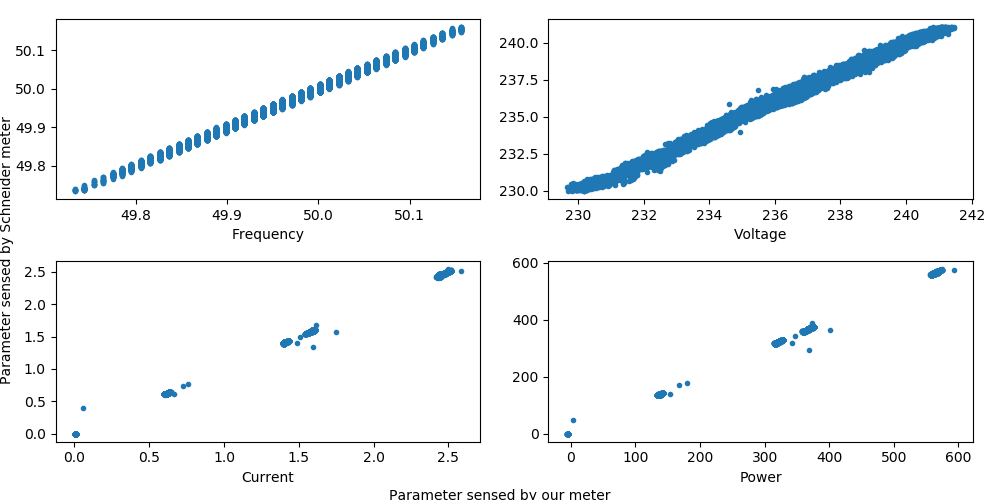
\includegraphics[width=1\linewidth]{images/fvcpcompare}
	\caption[Values observed by the new meter as compared with chneider meter]{Values observed by the new meter as compared with chneider meter}
	\label{fig:fvcpcompare}
\end{figure}

Correctly timestamped data is crucial when we have to compare the data from two meters. {Raspberry Pi }queries multiple meters at a rate faster than the sampling rate of the meter, this may result in a delay of up to one second in reading the data. The meters are not synchronized with each other therefore the transition may get observed in different cycles in different meters. Because of this reason, it is impossible to avoid a discrepancy of 1 to 2 seconds when a transition is observed at two different meters.


\begin{table}[h]
		\centering
		\caption{Correlation coefficient of unknown phase with 3 phases at \textit{Mains} meter.}
		\begin{tabular}{ccc}
			\hline
			$v_1$ & $v_2$ & $v_3$  \\
			\hline
			0.9808 & -0.1732 & -0.1618 \\
			\hline
		\end{tabular}
        %k what does that mean?
		\label{tab:corr_coef}
	\end{table}

	A larger timestamp discrepancy is also observed in the data when a Raspberry Pi is offline or is not able to update its timestamp from the server. Updating local time from NTP server requires direct or indirect Internet access, which may not be possible in some cases which can make the timestamp unreliable. Thus a mechanism other than one based on timestamps is required to make sure that the data from multiple meters pertains to the same time instance.

 The frequency of the supply voltage is maintained within a narrow range by the power generating systems. The system frequency plays a crucial role in meeting the power demand. The frequency of the power supply can be measured at any point in the electrical grid and will be the same everywhere  in the system. Whenever the load increases, the frequency decreases, this is detected by the generating systems and the power generation level is increased accordingly. This balancing is controlled by a speed governor installed at each generator.

	The change in the system frequency is minimal, but it is possible to measure it with very high precision. \textit{This frequency of the supply is measured by sensing voltage;} therefore, no additional hardware is needed to measure it. Figure \ref{fig:tsCorrection} shows the frequency measured by different meters during a short interval where timestamp of one meter is slightly out of sync with the other meters. We utilize this slight variation in the frequency to identify and correct any time difference in the data collected from different smart meters.

	Our objective is to identify the outliers and to recover the correct timestamp for such cases. Figure \ref{fig:tsCorrection} shows frequency samples taken from four meters. Meter 4 frequency data is not in alignment with the other meters; this is because of incorrect timestamp on this meter's data. As we do not know the source of  the misaligned data we compute the median frequency. Our objective is to find the best match for  meter 4 frequency data with the median frequency data. The intuition is to slide the meter 4 frequency data on the graph such that two waveforms coincide with each other. To check the alignment of the two waveforms the following optimization objective is used
	\begin{equation}
		\min_{0 \leq t_c \leq t_{max}}  \sum_{t=1}^{t_{max}}  \sqrt{abs(f_m(t)^2 - f_n(t + t_c)^2)}
	\end{equation}where $f_m(t)$ is the median frequency at time $t$ and $f_n(t)$ is the frequency measured at meter $n$ at time instance $t$. The cost function forms a $U$ shaped curve which makes it possible to use gradient descent to find the optimal value for $t_c$.
% rg
The algorithm is capable of correcting timestamp errors of duration up to $t_{max} / 2$.
%rg end
The procedure can be summarized as follows
	\begin{itemize}
		\item Take data sample for interval $t$ from each meter.
		\item Find the median frequency $f_m(t)$ for each timestamp.
		\item Minimize the cost function to find the value of $t_c$. If $t_c$ is zero the timestamp of the given sample is correct,  else it is used to time shift the data collected from the meter.
	\end{itemize}

Timestamp correction is performed as part of the data cleaning process each time meter data is used.



\begin{figure} 
	\centering
	\includegraphics[width=1\linewidth]{images/tsCorrection}
	\caption[Frequency Values sensed at different meters indicate that timestamp for meter 4 is incorrect]{Frequency Values sensed at different meters indicate that timestamp for meter 4 is incorrect}
	\label{fig:tsCorrection}
\end{figure}

\section{Labeling Error}
Sometimes it is observed that data belonging to one meter is labeled as another meter data and logged into that meter database. This happens because rs485 cable is shared for multiple meters and response from a smart meter may take too long and gets interpreted as response of the next request. The total energy consumption of each of the meter is at different levels, because of which this error is possible to identify and recover.

Energy value for one of the meters will be higher than the others, therefore a sudden increase and decrease in the energy value will be observed when this error happens. As it is impossible to have a drop in the energy value, and the magnitude is more than the power consumption in the meter, it can be concluded that data from other meter is present.
Algorithm for removing other meter data is as follows

If energy is beyond the minimum and the maximum possible value discard it. The lower data belongs to the meter being sensed while the higher one is of another meter.

\begin{algorithm}
	\caption{Algorithm to remove other meter data}
	\label{algo:Algorithmtoremoveothermeterdata}
	\begin{algorithmic}[1] % The number tells where the line numbering should start
		\State $E_{max} = E_{prev} + P_{max} * t_{elapsed}$
		\State $E_{min} = E_{prev}$
		%\If {$E_{sensed} le E_{max}  \and  E_{sensed} ge E_{min}$}
		\If {$E_{sensed} \le E_{max} \And E_{sensed} \ge E_{min}$}
			\State $save data$ 
			\State $E_{prev} = E_{sensed}$
		\Else
			\State $discard data$
		\EndIf
	\end{algorithmic}
\end{algorithm}

\section{Duplicate Data}
Even when the data is sorted, the presence of duplicate sample or presence of two samples at one timestamp will create problem while joining multiple meter data. To complete the drop in voltage at a given time, the voltage measured at two places should be compared. If all the meters meter had two records for a timestamp, joining the data from two meters will produce a total of $2^n$ records, which is the cartesian products. This causes two problems in the analysis.
    Memory requirement grows exponentially
    Learning gets skewed when different records get duplicated a different number of times.

As the data is already sorted duplicate data removal should satisfy the following two rules:
\begin{enumerate}
 \item No data should be repeated
 \item No timestamp should have more than one record for a meter
\end{enumerate}

duplicates are removed using algorithm \ref{algo:duplicate}

\section{Results and Data Samples}
Industrial meters like Schneider EM6400 \cite{EM6400MultifunctionMeter} use the slow Modbus interface to transfer the power consumption data. Modbus protocol works over the RS485 serial bus which is a half-duplex and supports slow data transfer rate typically 19.2 Kbps. All the communications on the RS485 bus are initiated by a master. I smart meter case the master sends a  request and the meter responds by sending the latest readings back.

In Modbus communication, the master is unaware of the state of the meter and does not know when the meter reading has changed. When data is required to be collected at 1 Hz rate, which is the same as the meter's refresh rate, the master should request the dare at a faster rate to avoid looking some intermediate meter readings. If identical reading is received such readings are discarded. The Modbus communication is initiated by the master, therefore, it is efficient for the regular interval query which is slower than the data refresh rate but is highly inefficient in other cases.

When the objective of installing the meter is to identify maximum and minimum power consumption during a period for the purpose of billing or to identify the time when the power consumption has changed for the purpose of disaggregation, it is highly inefficient to read power consumption from the meter every second. As the meter can compute such information very easily, changing the way in which data reading is performed can drastically reduce the communication overhead.

RS485 and thus Modbus can support up to 255 devices on a single bus but this number reduces drastically when data is collected at 1 Hz frequency. In Modbus protocol, when the power data is collected at the same rate as data refresh rate the master should query the meter with a faster rate than the data refresh rate to avoid missed data and discard the duplicate data received. This causes additional communication overhead and the communication channel is 100\% utilized when as few as 5-6 meters are connected on a single RS485 bus.

Our meter is capable of detecting the change in different parameters sensed and initiate the high frequency and the low-frequency communication based on these events. The possible events that can be used in the meter are threshold based change event and timer based events. These events can be used to collect the 1Hz or lower frequency power data or high-frequency current, voltage, and power samples.



\begin{figure} 
	\centering
	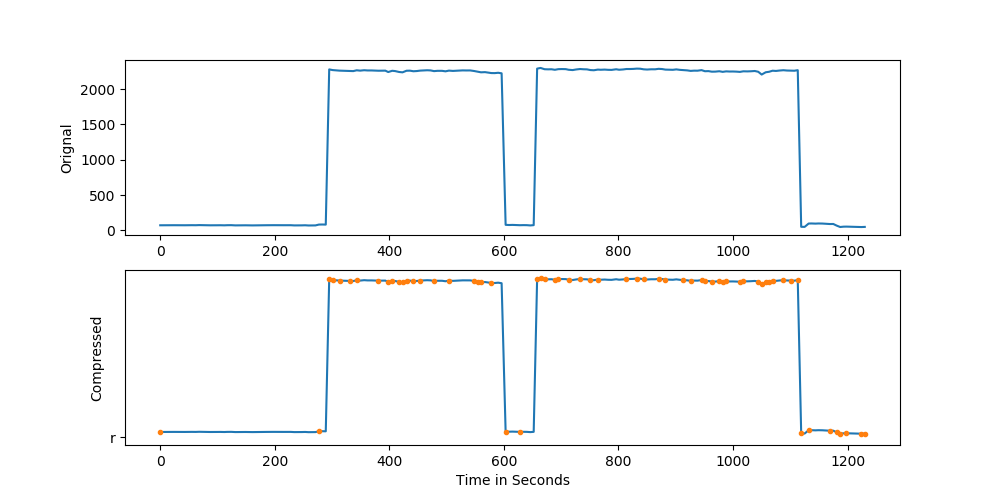
\includegraphics[width=1\linewidth]{images/compressRish}
	\caption[Power readings sent only 63 times instead of 1250 times]{Power readings sent only 63 times instead of 1250 times}
	\label{fig:compressRish}
\end{figure}

An energy meter senses the consumption of power for every cycle. Data collected for the duration of one second is then aggregated to obtain the power consumption for the second. This data can be queried from the Industrial meters using the MODBUS or similar such protocols. When per-second data is collected, the data volume is too high for large scale deployment. The change in power consumption is less frequent as the state of an appliance does not change very frequently. Smart meters installed in homes send the data at a much lower rate at an interval of 5-15 minutes. When the energy data is sent at such a lower rate all the information about the transients is missed out. As our meter holds the power consumption for every second and it relays the information whenever the changes in power consumption are significant enough. The number of messages required to send the change in power together with the 15-minute interval energy reading is significantly lower than the messages sent every second. We analyzed one-month data from 50 homes to evaluate our messaging strategy. We found that 3000 messages are sufficient to rebuild the per-second level power consumption details for 91\% of the cases. Figure \ref{fig:compressRish} shows the power consumption profile of one of the houses. The first graph is drawn using 1250 samples while the second one is drawn using only 63 samples. There was no significant difference between the two profiles. We can achieve this reduction in the data transfer because the communication is initiated by the meter and not by the master.


When a 1 Hz sample of power is used for energy disaggregation it is like taking a low resolution image of an object. The 1 Hz does not capture the complete details of the event that happens at the transition. Sometimes the events are entirely missed out because the averaging will reduce the intensity of the event. Some events are short-lived and are difficult to capture with 1-second samples. Our meter can provide the cycle level power consumption data that can provide better insight into such events. As these signals are sent when the change in power is detected, there is no chance of missing out on these events. Figure \ref{fig:H3Vacuum}, \ref{fig:H6AC}, \ref{fig:H10Microwave}, \ref{fig:H23WashingMachine} shows the comparison of a vacuum cleaner, air conditioner, microwave, and washing machine power data collected at 1 Hz and 50 Hz.

\begin{figure} 
	\centering
	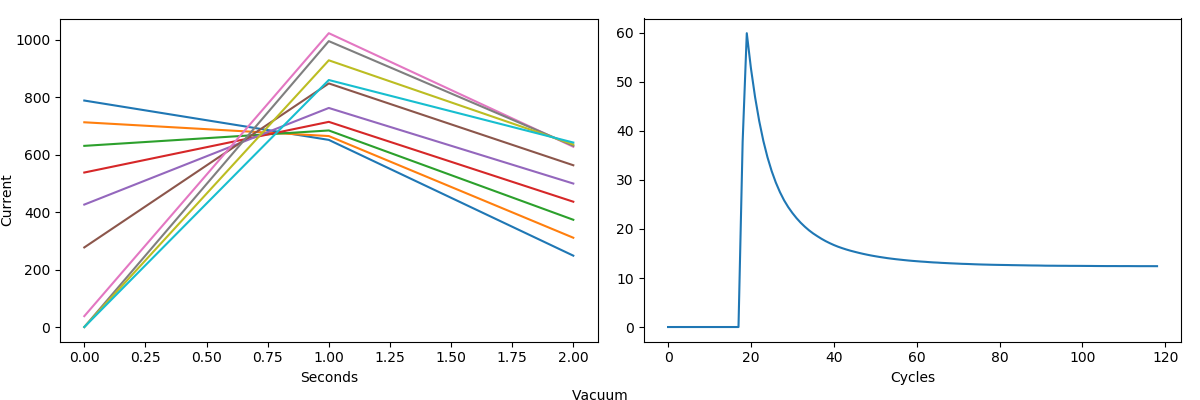
\includegraphics[width=1\linewidth]{images/H3Vacuum}
	\caption[1 Hz vs Cycle level signature provided by the meter for Vacuum]{1 Hz vs Cycle level signature provided by the meter for Vacuum}
	\label{fig:H3Vacuum}
\end{figure}

\begin{figure} 
	\centering
	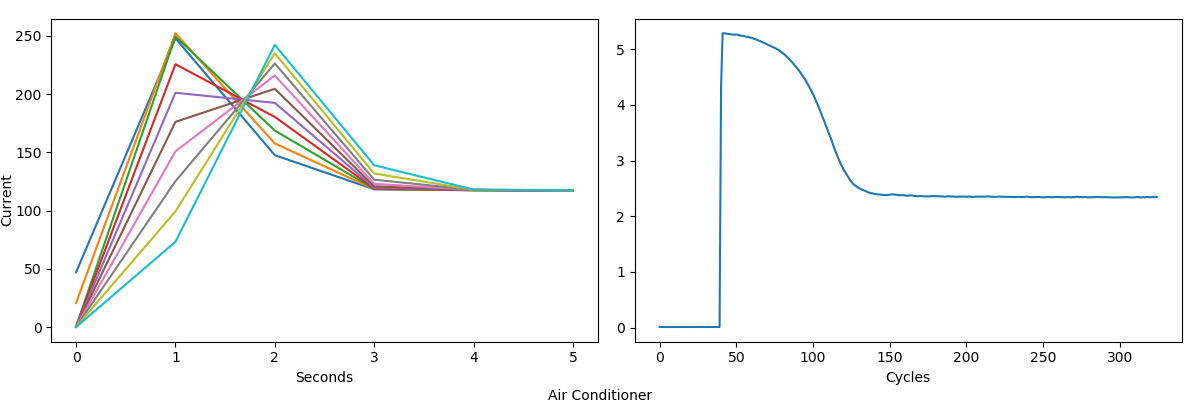
\includegraphics[width=1\linewidth]{images/H6AC}
	\caption[1 Hz vs Cycle level signature provided by the meter for Air Conditioner]{1 Hz vs Cycle level signature provided by the meter for Air Conditioner}
	\label{fig:H6AC}
\end{figure}

\begin{figure} 
	\centering
	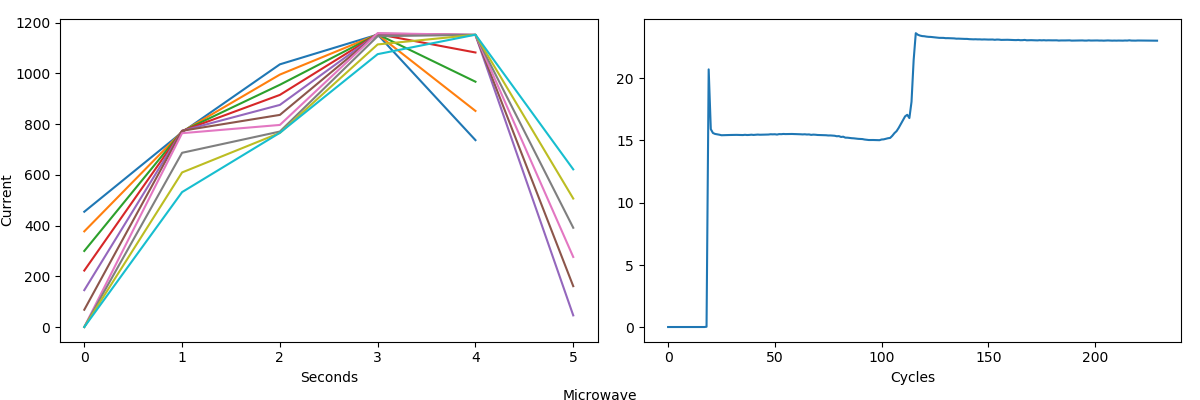
\includegraphics[width=1\linewidth]{images/H10Microwave}
	\caption[1 Hz vs Cycle level signature provided by the meter for Microwave]{1 Hz vs Cycle level signature provided by the meter for Microwave}
	\label{fig:H10Microwave}
\end{figure}

\begin{figure} 
	\centering
	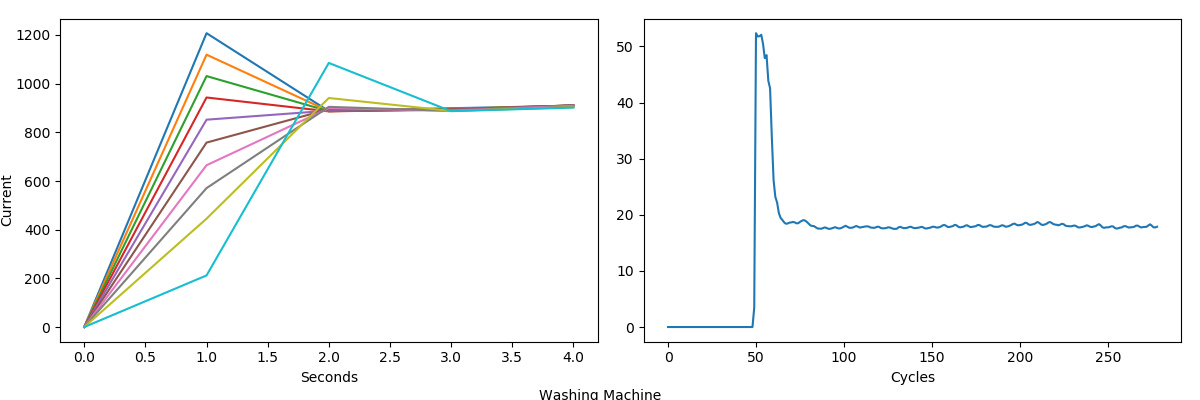
\includegraphics[width=1\linewidth]{images/H23WashingMachine}
	\caption[1 Hz vs Cycle level signature provided by the meter for Washing Machine]{1 Hz vs Cycle level signature provided by the meter for Washing Machine}
	\label{fig:H23WashingMachine}
\end{figure}

Many disaggregation techniques use high-frequency voltage and current data. Our meter is capable of collecting and providing 9.6 kHz voltage, current, and power data which can be used by many such techniques. We have collected such data for a variety of appliances.

Figure \ref{fig:hfCurrent} shows the high-frequency current data collected for four different types of appliances which is iron, fridge, a microwave, and a laptop. The current drawn by the iron is almost identical to the voltage waveform. this indicates that the iron is a pure resistive type of load.
The current drawn by the laptop is remains zero for the initial part of the cycle and shoots up at a certain input voltage. This is the typical characteristic of the AC to DC converters. We expected the current drawn from the fridge to be a shifted sinusoidal but it has some unexpected shape. On investigation, we found out this is because of the third harmonic. The current waveform of the microwave is also as expected.

Figure \ref{fig:hfVI} shows the VI-trajectory drawn by plotting v on the x-axis and current on the y-axis for the same four appliances. The VI-trajectory for the iron is almost a straight line which also indicates that the iron is a pure resistive type of load. The current VI-trajectory for the laptop has a sudden jump at both the highest voltage values. This is the typical characteristic of the AC to DC converters. The VI-trajectory for the fridge is a distorted oval which indicates that it is an inductive load. The VI-trajectory for the microwave is a galaxy like shape as expected.


\begin{figure} 
	\centering
	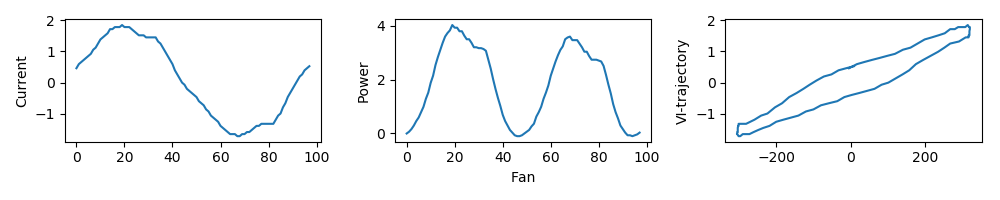
\includegraphics[width=1\linewidth]{images/fan10A2311}
	\caption[High-frequency data for Fan]{High-frequency data for Fan}
	\label{fig:fan10A2311}
\end{figure}

\begin{figure} 
	\centering
	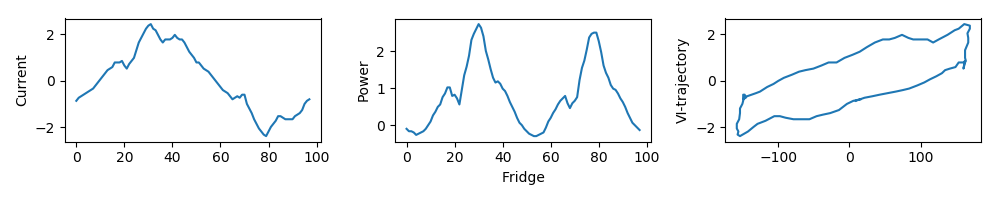
\includegraphics[width=1\linewidth]{images/fridge40A122}
	\caption[High-frequency data for Fridge]{High-frequency data for Fridge}
	\label{fig:fridge40A122}
\end{figure}

\begin{figure} 
	\centering
	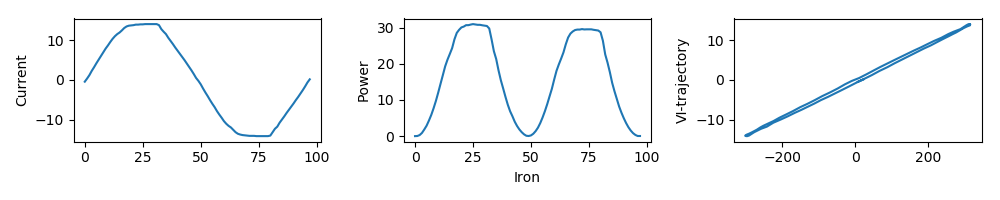
\includegraphics[width=1\linewidth]{images/iron40A2}
	\caption[High-frequency data for Iron]{High-frequency data for Iron}
	\label{fig:iron40A2}
\end{figure}

\begin{figure} 
	\centering
	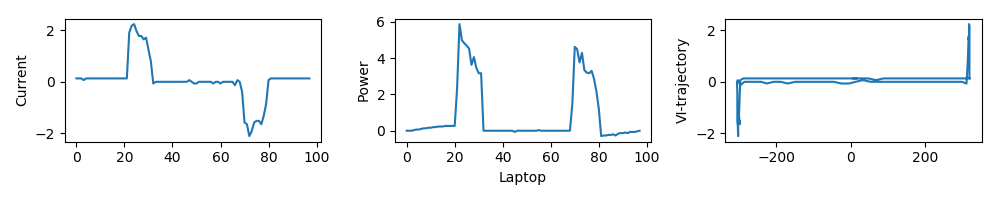
\includegraphics[width=1\linewidth]{images/Laptop10A1}
	\caption[High-frequency data for Laptop]{High-frequency data for Laptop}
	\label{fig:Laptop10A1}
\end{figure}

\begin{figure} 
	\centering
	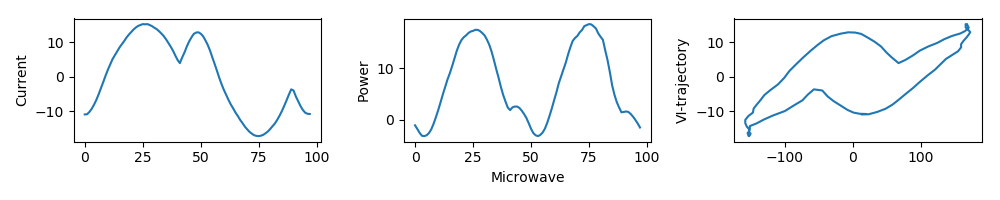
\includegraphics[width=1\linewidth]{images/microwave40A1}
	\caption[High-frequency data for Microwave]{High-frequency data for Microwave}
	\label{fig:microwave40A1}
\end{figure}

Our lab has three parallel supplies for plugs, fittings like lights and fans, and for air conditioners. We have installed the Schneider EM6400 meters to monitor and collect power consumption data at a frequency of one Hz. This data is collected by a raspberry-pi and sent to MQTT server from where different applications like database logger or data analyzer to subscribe to this data. We have installed our meters in In parallel with the Schneider EM6400 meter that collects the data for the fittings. We have selected this meter because we can easily get downtime and a number of different available power consumption levels observed in this meter.

We collected data from our meters at the rate of 1 sample per second and sent to the MQTT server similar to the Schneider meter. We compared the data for a number of days and analyzed the difference between the voltage, current, power, and frequency observed by the two meters. Figure \ref{fig:fvcpcompare} shows the comparison of the four parameters observed by the two meters for a period of one day. Table \ref{tab:rmsError} shows that the average of the absolute error is very low for all the parameters. The parameters observed by the two masters are almost identical except for occasional slight differences. Explanation of the observations is as follows.

Frequency:  No significant difference was observed in the frequency measured by the two meters.

Current: The current measured by the two meters is almost always the same except for the cases except for very few samples. This difference is only observed when some appliance is switched ON or OFF. Sometimes there is a delay in the Schnieder meter reporting the new current value. One of the reason could be because of the delay in querying the readings from through the MODBUS protocol. As the raspberry-pi adds the timestamp to the data when it is received from the meter, the timestamp is always delayed by a few hundred milliseconds.

Active Power: The active power measured by the two meters is almost identical except for a few cases similar to the current measurement. Active power is not a product of RMS voltage and current but is also a function of the power factor of the load. Our load of fans is a reactive load which indicates that the measurement of active power is accurate in case of such loads also.

Voltage: On the larger range the voltage change in the same range but there is always a slight difference in the readings collected from the two meters. It is observed that reading of one meter follows the reading of another meter. The sampling in the two meters does not start at the same cycle therefore even if the two meters are measuring the same value the average taken across 50/60 different cycles will be slightly different. As the voltage is continuously changing the values measured by any two meters will always differ slightly.


	In large buildings where a lot of similar appliances are installed, disaggregation of the appliance load is a challenging task. Utilization of already installed instruments can be a big factor in deciding the practical feasibility and success of such tasks.
Both voltage and current sensing have their own advantages in different places. Current sensing can be easy if no sockets are available and phase wires are accessible separately to install a clamp on current transformers. Voltage sensing, on the other hand, can reduce time and cost of installation or it can even eliminate by utilizing the voltage sensed by the already installed smart meters. It can also provide ad-hoc measurements through sockets for quick fault localization.

In this work, we exploit the fact that change in an appliance's power consumption will result in a change in the current flow and voltage drop at different places in the electrical system. Simple sensors can be installed to measure these changes and identify the appliance status. We have also presented a novel technique that uses sensed voltage and utilizes it to improve disaggregation results. We also presented an algorithm to decide about the placement of these sensors to yield maximum insight into the systems.

During this process, we experienced a lot of data collection challenges which we overcame using the sensed voltage. We have developed a robust sensor data logging system capable of automatic configuration and correction of time stamping and phase labeling errors.  The latter problem is encountered quite often in practice but has not been explicitly studied for buildings.  For example,  when we install solar roof-tops both in residences and in larger buildings, we need to ensure that a panel is connected to the right phase. In fact, most building managers have an incorrect circuit map of the building which can be quite large \& complex in commercial buildings. So identifying phase at every point and socket correctly is an important aspect of correcting the circuit map of a large building. Since buildings are also commercially billed, they are penalized for imbalanced phases by the utility that one cannot address without identifying the phase of different loads in the building.

We have made a strong case for voltage sensing which is capable of providing a lot of insights into the system. We showed that already installed hardware along with some additional voltage sensors, can be utilized to gain more insight into the system, one such insight leads to effective fault localization. These techniques can provide even better results by utilizing more precise voltage sensors.

For the realization of the smart grid, a large number of smart meters will be installed. The smart meters may become one with the highest penetrated smart devices of the different type of devices in the world because every household which uses electricity will have them. In the future, smart meters should be taking the role of being more than just the measurements devices. They may have a lot of features we cannot imagine now. A lot of research is needed to develop such a smart meter. We have presented a smart meter design that can act as a platform for future smart meter research. The presented smart meter design can be used for large scale deployment. It is an attempt towards making a device that can support not only the present smart grid but can easily support future needs.

Our smart meter is capable of providing high-frequency voltage, current and power data to perform energy disaggregation. This capability will enable the development of smart meters that can perform energy disaggregation without the help of any external processing resources. With such capabilities, it will be easy to enjoy a large acceptance by the end users.

It can support data communication initiated by the meter which drastically reduces the communication bandwidth requirement. This feature will reduce the overhead cost of large scale deployment of the smart meter. The presented meter is cost effective and can be assembled with ease as it uses the most easily available components. This will enable affordable large-scale deployment of smart meters.



	% \section{Problems in Finding Fault Location}


%=====================================================================
% APPENDIX
%****************************************************************
% %\appendix
\begin{appendices}
\chapter{}
\section{Symmetric Components}

\end{appendices}

%=====================================================================
% BIBLIOGRAPHY
%   This should follow the appendices, if any, otherwise summary and
%   conclusions chapter.
% Choose your bibliography style
% plain is the basic style, others include ieeetr, siam, asm, etc
\bibliographystyle{ieeetr}
%\bibliographystyle{IEEEtran}
%\bibliographystyle{acm}	
%\bibliographystyle{nature}
  
%******************************************************************
%                         Bibliography or References          
%******************************************************************  
\label{myreferences}
\bibliography{ref}

%*******************************************************************
%                         List of publications               
%******************************************************************
\include{chapters/mypublications}

%*******************************************************************
%                        Acknowledgements                    
%******************************************************************* 
\include{chapters/myacknowledgements}
\end{document}
